\documentclass[phd,bottom,nosig,dvipsnames]{usbthesis}

\usepackage{amsmath, amsthm, amssymb, bm}
\usepackage{dsfont}
\usepackage{physics}
\usepackage{units}

\usepackage{graphicx}
\graphicspath{{figures/}}
\usepackage{tikz-feynman}
\usepackage{tikz, pgfplots}
    \usetikzlibrary{arrows, intersections, math}
    \pgfplotsset{compat=1.15}
\usepackage{float}
\usepackage{subcaption}	% for subfigure
\usepackage[colorlinks]{hyperref}
% \usepackage{xcolor}
\hypersetup{
    colorlinks = true,
    urlcolor = [rgb]{0.85, 0.52, 0.9},
}
\usepackage{listings}
\lstset{
    % basicstyle=\linespread{0.6},
    % lineskip={0 pt},
    columns=fullflexible,
}
\usepackage[toc,page]{appendix}
% \usepackage{color}
\usepackage{setspace}
\usepackage{array}
\usepackage{lscape}
\usepackage{adjustbox}
\usepackage{tabularx}
\usepackage{tablefootnote}
\usepackage{multirow}
\usepackage{multicol}
\usepackage{makecell}
\usepackage{afterpage}
\usepackage{hhline}
\usepackage{url}
\usepackage{hyperref} % see the file hyperref.cfg for options
%\usepackage{indentfirst}
\usepackage{footmisc} % provides \footref and \mpfootnotemark commands
\usepackage{xspace} % ending space in custom macro
\usepackage[numbers,sort&compress]{natbib}
\usepackage{pdfpages}
%\usepackage[nottoc]{tocbibind}
\usepackage{comment}

\usepackage{indentfirst}
% This file defines a number of new commands and operators for nicer and more consistent math typesetting.
% Most are from http://www.tug.org/TUGboat/Articles/tb18-1/tb54becc.pdf

% similar-greater, similar-less
\def\simge{%
    \mathrel{\rlap{\raise 0.511ex
    \hbox{$>$}}{\lower 0.511ex \hbox{$\sim$}}}}
\def\simle{%
    \mathrel{\rlap{\raise 0.511ex
    \hbox{$<$}}{\lower 0.511ex \hbox{$\sim$}}}}

% make vectors bold, rather than using an arrow above
\renewcommand{\vec}[1]{\boldsymbol{#1}}

% Angstrom
\DeclareMathAccent{\ring}{\mathalpha}{operators}{"17}
\providecommand*{\angs}{\ensuremath{\smash{\mathrm{\ring A}}}}

% Ohm
\providecommand*{\ohm}{\ensuremath{\mathrm{\Omega}}}

% micro
\providecommand*{\micro}{\ensuremath{\mu}}

% micrometers
\providecommand*{\um}{\micro m}

% microseconds
\providecommand*{\us}{\micro s}

% Units
\providecommand*{\unit}[1]{\ensuremath{\mathrm{\,#1}}}

% The number `e'
\providecommand*{\eu}{\ensuremath{\mathrm{e}}}

% The imaginary unit
\providecommand*{\iu}{\ensuremath{\mathrm{i}}}

% text on exponent (superscript) level
\providecommand*{\apx}[1]{\ensuremath{^\mathrm{#1}}}

% text on index (subscript) level
\providecommand*{\ped}[1]{\ensuremath{_\mathrm{#1}}}

% degrees (for angles)
\providecommand*{\degree}{\ensuremath{^\circ}}

% degrees celsius
\providecommand*{\celsius}{\ensuremath{\mathrm{^\circ C}}}

% Real and Imaginary parts
\providecommand{\newoperator}[3]{\newcommand*{#1}{\mathop{#2}#3}}
\providecommand{\renewoperator}[3]{\renewcommand*{#1}{\mathop{#2}#3}}
\renewoperator{\Re}{\mathrm{Re}}{\nolimits}
\renewoperator{\Im}{\mathrm{Im}}{\nolimits}

% differential operator
\makeatletter
\providecommand*{\diff}{\@ifnextchar^{\DIfF}{\DIfF^{}}}
\def\DIfF^#1{\mathop{\mathrm{\mathstrut d}}\nolimits^{#1}\gobblespace}
\def\gobblespace{\futurelet\diffarg\opspace}
\def\opspace{%
    \let\DiffSpace\!%
    \ifx\diffarg(%
        \let\DiffSpace\relax
    \else
        \ifx\diffarg[%
            \let\DiffSpace\relax
        \else
            \ifx\diffarg\{%
                \let\DiffSpace\relax
            \fi\fi\fi\DiffSpace}

% total and partial derivatives
%   1st argument [] (optional): derivative order
%   2nd argument {}: function being derived
%   3rd argument {}: derivation variable
\providecommand*{\deriv}[3][]{\frac{\diff^{#1}#2}{\diff #3^{#1}}}
\providecommand*{\pderiv}[3][]{\frac{\partial^{#1}#2}{\partial
#3^{#1}}}


% Latin abbreviations
\providecommand*{\eg}{\emph{e.\,g.}\xspace}%
\providecommand*{\ie}{\emph{i.\,e.}\xspace}%

%\newcommand{\ket}[1]{\ensuremath{|{#1}\rangle}}
\newcommand{\one}{\ensuremath{\ket{1,-1}}}
\newcommand{\two}{\ensuremath{\ket{2,-2}}}
\newcommand{\probe}{\ket{p}}
\newcommand{\target}{\ket{t}}
\newcommand{\pro}{\ket{p}\xspace}
\newcommand{\tar}{\ket{t}\xspace}
\newcommand{\aat}{\ket{a}}
\newcommand{\bat}{\ket{b}}
\newcommand{\momz}{\ket{0}}
\newcommand{\momt}{\ket{\pm2}}
\newcommand{\mompt}{\ket{2}}
\newcommand{\mommt}{\ket{-2}}
\newcommand{\emphsection}[1]{\emph{#1}}

\newcommand{\CA}{\mathcal{A}}
\newcommand{\CH}{\mathcal{H}}
\newcommand{\CI}{\mathcal{I}}
\newcommand{\CK}{\mathcal{K}}
\newcommand{\CL}{\mathcal{L}}
\newcommand{\CM}{\mathcal{M}}
\newcommand{\CP}{\mathcal{P}}
% \newcommand{\H}{${}^{1}$H\xspace}
\newcommand{\He}{${}^{4}$He\xspace}
\newcommand{\Carbon}{${}^{12}$C\xspace}
\newcommand{\ca}{${}^{40}$Ca\xspace}
\newcommand{\Ca}{${}^{48}$Ca\xspace}
\newcommand{\Pb}{${}^{208}$Pb\xspace}
% \newcommand{\deg}{{}^\circ}

\newcommand{\goto}{\rightarrow}
\newcommand{\goback}{\leftarrow}
\newcommand{\Goto}{\Rightarrow}
\newcommand{\Goback}{\Leftarrow}
\newcommand{\Godown}{\Downarrow}

\newcommand{\AxisRotator}[1][rotate=0]{
    \tikz [x=0.2 cm, y=0.45 cm, line width=.2 ex, -stealth, #1] \draw (0, 0) arc (150:-150:1 and 1);
}
\newcommand{\AxisRotatorReversed}[1][rotate=0]{
    \tikz [x=0.2 cm, y=0.45 cm, line width=.2 ex, -stealth, #1] \draw (0, 0) arc (-150:150:1 and 1);
}
\newcommand*{\@rowstyle}{}

\newcommand*{\rowstyle}[1]{% sets the style of the next row
  \gdef\@rowstyle{#1}%
  \@rowstyle\ignorespaces%
}

\newcolumntype{=}{% resets the row style
  >{\gdef\@rowstyle{}}%
}

\newcolumntype{+}{% adds the current row style to the next column
  >{\@rowstyle}%
}


\definecolor{darkpink}{rgb}{.239, .027, .161}
\lstdefinestyle{C}{
    language=C,
    backgroundcolor=\color{darkpink},
    basicstyle=\ttfamily\footnotesize\singlespacing\color{white},
    % breakatwhitespace=false,
    commentstyle=\color{blue!60},
}

\hyphenation{put words here which LaTeX does not hy-phen-ate pro-per-ly}

\author{Weibin Zhang}%
\title{Precise Measurement of the Neutron Skin Thickness of $^{208}Pb$ and $^{48}Ca$}%

\month{June}
\year{2022}%
\program{Physics}%
\director{Abhay~Deshpande}{Professor, Department of Physics and Astronomy}%
%\chairman{Name of Chairman}{Professor, Department of Physics and Astronomy}%
\chairman{James~M.~Lattimer}{Professor, Department of Physics and Astronomy}%
%\outmember{Name of Outside Member}{Position}{Institution}%
\fstmember{Jiangyong~Jia}{Professor,  Department of Physics and Astronomy}%
%\fstmember{Name of Member}{Professor, Department of Physics and Astronomy}%
\outmember{Ciprian~Gal}{Assistant Research Professor}{Mississippi State University}%
\dean{Eric Wertheimer}%

\begin{document}

\singlespacing %
\pagenumbering{roman} %
\maketitle %
\makeapproval %

\begin{abstract}
Despite great leaps of development in nuclear physics over the past century, 
we still don’t have a comprehensive understanding of nuclear structure. This 
is mainly due to the lack of precise knowledge of neutron distribution inside nucleus. 
Electromagnetic probes are ineffective in probing neutrons, unlike their charged partners, 
the protons. Therefore, it is of great importance to constrain the neutron distributions experimentally. 
Heavy nuclei have more neutrons than protons in order to balance the repulsion between protons. 
In such neutron-rich nuclei, the extra neutrons are pushed out to the surface 
by the nuclear symmetry energy, forming the so-called ``neutron skin". 
The neutron skin can be probed with a well-established experimental technique 
-- parity-violating electron scattering (PVES). Using the scattering of 
longitudinally polarized electrons by an unpolarized target, PREX-II and CREX 
measure the small parity-violating asymmetry in cross sections. Employing 
electrons with opposite helicities the weak form factor, the neutron distribution 
and the neutron skin thickness of the target nucleus are extracted. 
With excellent beam qualities and dedicated instrumentation at Jefferson Lab, 
the asymmetry measurements are statistics-limited. We report the results of these 
two high-precision measurements and their implications on broad topics, 
from the nuclear structures to the neutron stars.

\end{abstract}
\tableofcontents %
\listoffigures %
%
%\listoftables %
%
\begin{acknowledgements}
    I hardly ever imagine the moment of completing my graduate studies, but here I am. 
I would not have made it this far without the invaluable and generous help and support from various 
individuals, including my supervisor, colleagues, friends and family.

I would like to express my deepest gratitude to my advisor, Dr. Abhay Deshpande
for his unwavering support throughout my Ph.D. studies, his meticulous care for me 
and his thoughtful guidance in my academic and research journey.

I still remember my first meet with Abhay in the small garden during a Friday social.
That was my first month at Stony Brook and I was even not very fluent in English.
Abhay warmly introduced his research and invited me to talk to him later, that 
was how I knew him and joined his group for my Ph.D. study. Obviously, he is super busy 
that I was first working with KK and then Ciprian, and finally Abhay himself. 
That does not mean he is neglecting his students. Actually, you can ask for 
his suggestions or helps whenever he is available, that is also what he always 
encourages us to do and what I would urge you to do, whenever you have a chance to talk to him.

I would like to extend my sincere thanks to Dr. Ciprian Gal, for his 
invaluable guidance and support in the PREX-II/CREX experiments. His expertise 
and advice regarding research have been instrumental in shaping my studies. 
Additionally, I am truly thankful for his assistance in various aspects of my work.
I want to extend my thanks to Dr. Sanghwa Park for her help during the experiment
and the contamination analysis afterward. It is highly beneficial to
work with them.

I would like to thank Dr. Krishna Kumar, Dr. Kent Paschke, Dr. Paul King
and all the other spokespersons of the PREX-II/CREX Collaboration. It is a great honor
to be part of the collaboration. I am also grateful to every hard working postdoc and
graduate student, especially the SBU group, including Dr. Chandan Ghost, Tao Ye, Cameron 
Clarke, and Ryan Richard. Thank you for making the measurements high-precision.

I also want to thank my friends and colleagues here at Stony Brook and those in Newport News. 
The fun time with you is an indispensable supplement to the research.

Last but not least, I would like to thank my parents, sister and relatives.
Although I have not been able to meet them in person due to Covid, 
I can feel their presence around me, 
providing me with reliable support. Thank you so much!

\end{acknowledgements}
\pagestyle{thesis}
\newpage
\pagenumbering{arabic}
\setlength{\baselineskip}{15.pt}
% \chapter{Style}
\textbf{Remember to remove it after completing your thesis.}

\section{Geometry}
\begin{itemize}
    \item pdfpageheight (pdfpagewidth) -- \the\pdfpagewidth (\the\pdfpageheight) -- page height and width
    \item baselineskip -- \the\baselineskip -- vertical distance between two
	nearby lines; set it to change line gap
    \item left (right) margin -- 

\end{itemize}

%%%%%%%%%%%%%%%%%%%%%%%%%%%%%%%%%%%%%%%%%%%%%%%%%%%%%%%%%%%%%%%%%%%%%%%%
\section{Introduction}
% 1. neutron distribution
% 2. symmetry energy dependence on density

%%%%%%%%%%%%%%%%%%%%%%%%%%%%%%%%%%%%%%%%%%%%%%%%
\subsection{symmetry energy} 
% what's symmetry energy
% why it is important
% how to know/measure it -- theoritically and experimentally
It has long been a hot topic for nuclear scientists to study how the asymmetry 
between number of proton and nucleon will affect nuclei, especially the binding
energy, which hints us the limit of new isotope elements. Using the simplest 
liquid drop model, we will get the Bethe-Weizsacker Semi-empirical Mass Foumula:
\begin{equation}
    \label{eq:mass-foumula}
    \begin{gathered}
	E\ (MeV) = \textcolor{black}{a_V A} - \textcolor{blue}{a_S A^{2/3}} - \textcolor{green}{a_C\frac{Z(Z-1)}{A^{1/3}}} - \textcolor{red}{a_A\frac{(N-Z)^2}{A}} + \textcolor{cyan}{\delta(A, Z)} + \dots \\
	\delta(A, Z) = 
	    \begin{cases}
		+\delta_0	& \text{Z, N even} \\
		0		& \text{A odd}	\\
		-\delta_0	& \text{Z, N odd (A even)} \\
	    \end{cases}
    \end{gathered}
\end{equation}

\begin{itemize}
    \color{black} \item Volume term: nucleons attract nearest neighbors 
	through strong force ($a_V \sim 16\ MeV$)
    \color{blue}  \item Surface term: correction to the volume term -- nucleons 
	on the surface aren't completely surrounded by other nucleons
    \color{green} \item Coulomb term: electromagnetic (EM) charge repulsion
    \color{red}   \item Asymmetry term: Pauli exclusion principle
    \color{cyan}  \item Pairing term: spin coupling effect -- if N and Z are even,
	then the nuclei will be stable thanks to the occurance of 'paired spin';
	on the other hand, nuclei with odd number of proton and neutron are usually
	unstable. ($\delta_0 \sim 1\ MeV$, slowly decreasing with A)
\end{itemize}

The first 3 terms are natural and easy to understand, while the 4th term is 
not so obvious. It is based only on Pauli exclusion principle. In heavy nuclei,
more neutrons than protons are needed to balance the repulsion between protons.
Due to the Pauli exclusion principle, these extra neutrons' energy will be 
higher than the rest of nucleons, therefore introducing this correction term.

For a general discussion, we can ignore the 3rd term to focus on the homogeneous
nuclear (residual strong) interaction between nucleons, and the 5th term which is too small.
Now, we can talk about any nuclear system composed of Z protons (EM charge-less) 
and N neutrons, rather than just true nuclei. Now we have a simplified equation
of state (EoS) for nuclear matter:
\begin{equation}
    \label{eq:modified-mass-formula}
    \begin{aligned}
	E &= a_V A - a_S A^{2/3} - a_A\frac{(N-Z)^2}{A}  \\
	e &= \frac{E}{A} = a_V - a_S A^{-1/3} - a_A\frac{(N-Z)^2}{A^2} = E_0(A) - a_A\left(\frac{N-Z}{A}\right)^2 
    \end{aligned}
\end{equation}

We can see that the binding energy depends on two variables, N and Z; or N+Z (A)
and N-Z. If we fix A, then $e$ will be a solely function of N-Z, or conventionally
$\beta = (N-Z)/A$. $\beta$ characterizes the asymmetry between the number of 
protons and neutrons. Again, for the purpose of generalization, we will replace
N, Z and A with their corresponding density: $\rho_n$, $\rho_p$ and $\rho$
($\beta = \frac{\rho_n - \rho_p}{\rho}$). 
So we are considering a uniform nuclear system at 0 temperature that interacts
only via the nuclear force.
Rewrite eq \eqref{eq:modified-mass-formula}:
\begin{equation}
    \label{eq:symmetry-energy}
    e(\rho, \beta) = e(\rho, 0) + S(\rho)\beta^2 + O(\beta^4)
\end{equation}

This is the expansion of the binding energy per nucleon around $\beta = 0$.
Due to the isospin symmetry between proton and neutron, any isoscalar quantities
F will keep unchanged under $n \leftrightarrow p$ interchange, while isovector 
% change all n into p and p into n. Not just one proton and one neutron
quantities G will change sign. $\beta$ is a isovector, so for a smooth $F(\beta)$,
its expansion around $\beta = 0$ has even terms only:
$$ F(\beta) = F_0 + F_2\beta^2 + F_4\beta^4 + \dots $$
On the other hand, for a smooth $G(\beta)$, its expansion around $\beta = 0$ has
odd terms only:
$$ G(\beta) = G_1\beta + G_3\beta^3 + \dots $$

e is an isoscalar, it doesn't change under $n \leftrightarrow p$ interchange 
as we can see from eq \eqref{eq:modified-mass-formula}. The coefficient $S(\rho)$ is
what we call the \textbf{symmetry energy}, a key parameter in explaining a wide
range of nuclear properties and phenomena. It describes how much energy is needed
to exchange all protons into neutrons for a symmetric nuclear matter. Take 
neutron star \ref{Lattimer.2001} as an example, it has most neutrons and a few 
protons, so its $\beta = 1$.
$$ E = E_0 + S $$
$$ P = \rho^2 \frac{dS}{d\rho} \approx \frac{L\rho^2}{3\rho_0} $$
$$ RP^{-1/4} \approx const $$
Once we know symmetry energy's dependence on density, we will know the pressure
and therefore the radius of a neutron star.

Being such an important parameter, a great effort has been done to extract S 
and its dependence on $\rho$. By convention, $S(\rho)$ is expanded around the
nuclear saturation density $\rho_0$:
\begin{equation}
    S(\rho) = S(\rho_0) 
    + \left.\frac{dS}{d\rho}\right|_{\rho_0}(\rho - \rho_0)
    + \frac{1}{2}\left.\frac{d^2S}{d\rho^2}\right|_{\rho_0}(\rho - \rho_0)^2
    + \frac{1}{6}\left.\frac{d^3S}{d\rho^3}\right|_{\rho_0}(\rho - \rho_0)^3
    + \dots
\end{equation}
From which, we have some other parameters defined:
\begin{equation}
    \begin{aligned}
	S_0 &= S(\rho_0)	\\
	L   &= 3\rho_0\left.\frac{dS}{d\rho}\right|_{\rho_0}	\\
	K_{sym}	&= 9\rho_0^2\left.\frac{d^2S}{d\rho^2}\right|_{\rho_0}	\\
	Q_{sym}	&= 27\rho_0^3\left.\frac{d^3S}{d\rho^3}\right|_{\rho_0}	\\
    \end{aligned}
\end{equation}
$$ S(\rho) = -a_A + \frac{L}{3}\frac{\rho - \rho_0}{\rho_0} $$


% \begin{equation}
%     \begin{aligned}
% 	\frac{E_b}{A} &= -B + \frac{K_0}{18}\left(\frac{n}{n_s} - 1\right)^2 + \frac{K'_0}{162}\left(\frac{n}{n_s} - 1\right)^3 \\
% 	    &+ \left[S_v + \frac{n_s}{3n}L\left(\frac{n}{n_s} - 1 \right) + \dots \right] \left(\frac{N-Z}{A} \right)^2 + \dots
%     \end{aligned}
% \end{equation}
For symmetric nuclei (N = Z), 
While neutron-rich nuclei, the extra nutrons are
pushed out against the surface tension\cite{PRL.85.5296}, therefore the neutron skin.

% \begin
There has been many measurements (!!!FIXME!!!) about the charge form factor of many elements,
but rarely any precise measurement of the weak form factor of any elements.
The Pb Radius EXperiment-II (PREX-II) and Ca48 Radius EXperiment (CREX) are 
high-precision experiments that measures the tiny asymmetry of polarized electrons
scattered from neutron-rich targets to extract the weak form factor and neutron
skin thickness of those nuclei. 


With the high-polarization electron beam at 
Thomas Jefferson National Accelerator Facility (TJNAF, also known as Jlab), 
we were able to measure the asymmetry precisely. 
The cross section asymmetry comes from the interference between 
the electromagnetic (EM) interaction and the weak interaction. While the EM 
cross section has been studied thoroughly, (!!!FIXME!!!: reference) the asymmetry 
measurement allows us to derive the weak charge distribution and finally the
neutron distribution in a nuclear.

The neutron skin of heavy nuclei and neutron stars, though of their 18 orders of 
magnitude difference in size (fm vs km), both are neutron-rich matter and thereby
governed by the same physical laws: the nuclear equation of state. 
The measurement of neutron radius of neutron-rich nuclei will constrain 
the density dependence of the symmetry energy for neutron-rich matter,
(!!!FIXME: reference)
it helps to identify the Equation of State (EoS) of neutron stars.

There have been many explorations from different aspects to the neutron skin
thickness: hadronic scattering experiment, coherent pion photoproduction,
measurements of electric dipole polarizabilities and pygmy dipole resonances etc.
Though of their valuable efforts, these experiments are trapped by model 
dependence and other uncertainties.


%%%%%%%%%%%%%%%%%%%%%%%%%%%%%%%%%%%%%%%%%%%%%%%%
\subsection{Asymmetry}
\feynmandiagram[small, vertical' = a to b]{
    i1 [particle = $e^-$] -- [fermion] a -- [fermion] o1 [particle = $e^-$],
    a -- [photon, edge label={Q}, edge label'=$\gamma$] b,
    i2 [particle = p] -- [fermion] b -- [fermion] o2 [particle = p],
    };
\feynmandiagram[small, vertical' = a to b]{
    i1 [particle = $e^-$] -- [fermion] a -- [fermion] o1 [particle = $e^-$],
    a -- [scalar, edge label={Q}, edge label'=Z] b,
    i2 [particle = p] -- [fermion] b -- [fermion] o2 [particle = p],
    };

\begin{itemize}
    \item $\gamma$ interacts with only vector current
    \item while $Z_0$ interacts with both vector and axial-vector current
\end{itemize}

\begin{equation*}
    \CA_{pv} = \frac{\frac{d\sigma^R}{d\Omega} - \frac{d\sigma^L}{d\Omega}}{\frac{d\sigma^R}{d\Omega} + \frac{d\sigma^L}{d\Omega}} = \frac{|\CM^R|^2 - |\CM^L|^2}{|\CM^R|^2 + |\CM^L|^2}
\end{equation*}
where: $\CM^{R, L} = \CM_{\gamma} + \CM_Z^{R,L}$

\begin{equation*}
    \begin{aligned}
	|\CM^{R,L}|^2 &= |\CM_\gamma|^2 + \CM_\gamma\CM_Z^{R,L*} + \CM_\gamma^*\CM_Z^{R,L} + |\CM^{R,L}|^2	\\
	|\CM^{R}|^2 - |\CM^{L}|^2 &= \CM_\gamma( \CM_Z^{R*} - \CM_Z^{L*} + \CM_Z^{R} - \CM_Z^L) \\
	&\approx 2\CM_\gamma(\CM_Z^R - \CM_Z^L)
    \end{aligned}
\end{equation*}


\begin{equation*}
    \begin{aligned}
	\CA_{pv}\footnotemark &\approx \frac{\CM_Z^R - \CM_Z^L}{\CM_\gamma} \propto \frac{\frac{d\sigma_{\text{weak}}}{d\Omega}}{\frac{d\sigma_{\text{E+M}}}{d\Omega}}	\\
	    &\approx \frac{G_F Q^2}{4\pi\alpha\sqrt{2}} \frac{Q_{wk}}{Z}\frac{F_{wk}(Q^2)}{F_{ch}(Q^2)}
    \end{aligned}
\end{equation*}
\begin{equation*}
    \begin{aligned}
	F_{ch}(q) &= G_{ch}^p(q)F_p(q) + G_{ch}^n(q)F_n(q)  \\
		  &= G_E^p(q)F_p(q) + \frac{N}{Z}G_E^n(q)F_n(q)	\\
	F_{wk}(q) &= G_{wk}^p(q)F_p(q) + G_{wk}^n(q)F_n(q)  \\
		  &= G_E^p(q)\left[ F_n(q) - \frac{Z}{N}(1-4\sin^2\theta_W)F_p(q)\right] - G_E^n(q)\left[ F_n(q)(1-4\sin^2\theta_W) - \frac{Z}{N}F_p(q)\right]
    \end{aligned}
\end{equation*}
Where $G_E^p(q)$ and $G_E^n(q)$ are the EW single nucleon FFs, $\sin^2\theta_W = 0.23$ is the Weinberg angle, $F_p(q)$ and $F_n(q)$ are the FFs of point proton and neutron density dist. Compared with $G_E^p(q)$, the charge FF of the neutron $G_E^n(q)$ can be neglected for small momentum transfer:
\begin{equation*}
    \begin{aligned}
	F_p(q) &= \int d^3r j_0(qr) \rho_p(r)	\\
	F_n(q) &= \int d^3r j_0(qr) \rho_n(r)	\\
	G_{wk}^p &= q_p G_E^p + q_n G_E^n + q_0 G_E^s	\\
	G_{wk}^n &= q_p G_E^p + q_n G_E^n + q_0 G_E^s	\\
    \end{aligned}
\end{equation*}
For weak charges including radiative cor.
$$ q_p \approx 0.0712	\qquad q_n = q_0 \approx -0.9877 $$
$$ \frac{F_{wk}(q)}{F_{ch}(q)} \approx \frac{F_n(q)}{F_p(q)}$$
$$ \CA_{pv} = \frac{G_FQ^2}{4\pi\alpha\sqrt{2}}\frac{Q_{wk}}{Z}\left[ \frac{F_n(q)}{F_p(q)} - \frac{Z}{N}(1-4\sin^2\theta_W) \right]$$
where: $F(Q^2) = \int d^3r \frac{sin(Qr)}{Qr}\rho(r)$
\begin{equation*}
    \rho(\vec{r}) = Q^{N}\rho_N(\vec{r}) + Q^{P}\rho_P(\vec{r})
\end{equation*}
In general use model for $\rho(\vec{r})$, example: Wood-Saxon form:
\begin{equation*}
    \rho(r) = \frac{\rho_0}{1 + exp[(r-R)/a]}
\end{equation*}
where R is the radius of the density $\rho(r)$?

\bigskip
When ignoring structure (tree level):
\begin{equation*}
    \CA_{\text{pv}} = \frac{G_F Q^2}{\pi\alpha\sqrt{2}} \left(\sin^2\theta_W + \frac{1}{4}\left[ \frac{N}{Z} - 1 \right] \right)
\end{equation*}
\footnotetext[1]{
    for low $Q^2$:
    \begin{equation*}
	\CA_{pv} = \frac{G_F Q^2}{4\pi\alpha\sqrt{2}} \left[ 1- 4\sin^2\theta_W - \frac{F_n(Q^2)}{F_p(Q^2)} \right]
    \end{equation*}
}

\begin{equation*}
    Q_{\text{weak}}^{p} \propto 1 - 4\sin^2\theta_{\text{W}} \approx 0.076
    \quad
    Q_{\text{weak}}^{n} \propto -1
\end{equation*}
\begin{equation*}
    \sigma_{\text{raw}} = \sigma_{\text{sig}} + \sigma_{\text{other}} + \sigma_{\text{HC}}
\end{equation*}

\begin{equation*}
    \begin{aligned}
	\CA_{\text{pv, measured}} &= \frac{(\sigma_{\text{sig}}^R + \sigma_{\text{other}}^R + \sigma_{\text{HC}}^R) - (\sigma_{\text{sig}}^L + \sigma_{\text{other}}^L - \sigma_{\text{HC}}^L)}{(\sigma_{\text{sig}}^R + \sigma_{\text{other}}^R + \sigma_{\text{HC}}^R) + (\sigma_{\text{sig}}^L + \sigma_{\text{other}}^L - \sigma_{\text{HC}}^L)}    \\
	&\approx \CA_{\text{pv, true}}\left( 1 - \frac{\sigma_{\text{other}}^R + \sigma_{\text{other}}^L}{\sigma_{\text{sig}}^R + \sigma_{\text{sig}}^L} \right) + \frac{\sigma_{\text{HC}}^R + \sigma_{\text{HC}}^L}{\sigma_{\text{sig}}^R + \sigma_{\text{sig}}^L} 
    \end{aligned}
\end{equation*}

\subsection{Dynamics}
\begin{center}
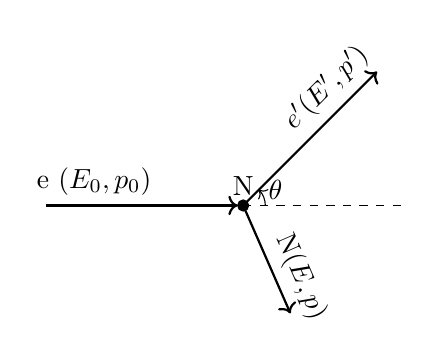
\begin{tikzpicture}
    \coordinate (N) at (0, 0);
    \coordinate (ein) at (-2.5, 0);
    \coordinate (eout) at (1.7, 1.7);
    \coordinate (p) at (0.6, -1.37);

    \filldraw[black] (N) circle (2pt);
    \node [above] at (N) {N};
    \draw[->, thick] (ein) -- node [near start, above] {e ($E_0, p_0$)} ([xshift=-2pt]N);
    \draw[dashed] (N.east) -- +(2, 0);
    \draw[->, thick] (N) -- node[near end, above, sloped] {$e' (E', p')$} (eout);
    \draw[->, thick] (N) -- node[near end, above, sloped] {N($E, p$)} (p);
    \draw [->] ([xshift=8pt]N) arc (0:45:8pt) node[right] {$\theta$};
\end{tikzpicture}
\end{center}

4-Momentum conservation 
$$ E_0 + M = E' + E \qquad \vec{p}_0 = \vec{p}' + \vec{p} $$
Assume ($m_e << 0 \Rightarrow E_0 \approx p_0, E' \approx p'$)
\begin{equation*}
    \begin{aligned}
	E^2 &= M^2 + \vec{p}^2 = M^2 + (\vec{p}_0 - \vec{p}')^2  \\
	    &= M^2 + (E_0 - E'\cos\theta)^2 + (E'\sin\theta)^2	\\
	    &= M^2 + E_0^2 + E'^2 - 2E_0E'\cos\theta	\\
	    &= (E_0 + M - E')^2
    \end{aligned}
\end{equation*}
So we can get
$$ M(E_0 - E') = E_0E'(1-\cos\theta) $$
$$ E' = \frac{ME_0}{M + E_0(1-\cos\theta)}$$
\begin{equation*}
    \begin{aligned}
	Q^2 &= (E_0 - E')^2 - (\vec{p}_0 - \vec{p}')^2	\\
	    &= -2E_0E'(1-\cos\theta)
    \end{aligned}
\end{equation*}

%%%%%%%%%%%%%%%%%%%%%%%%
\subsubsection{Why \Pb and \Ca}
\begin{figure}
    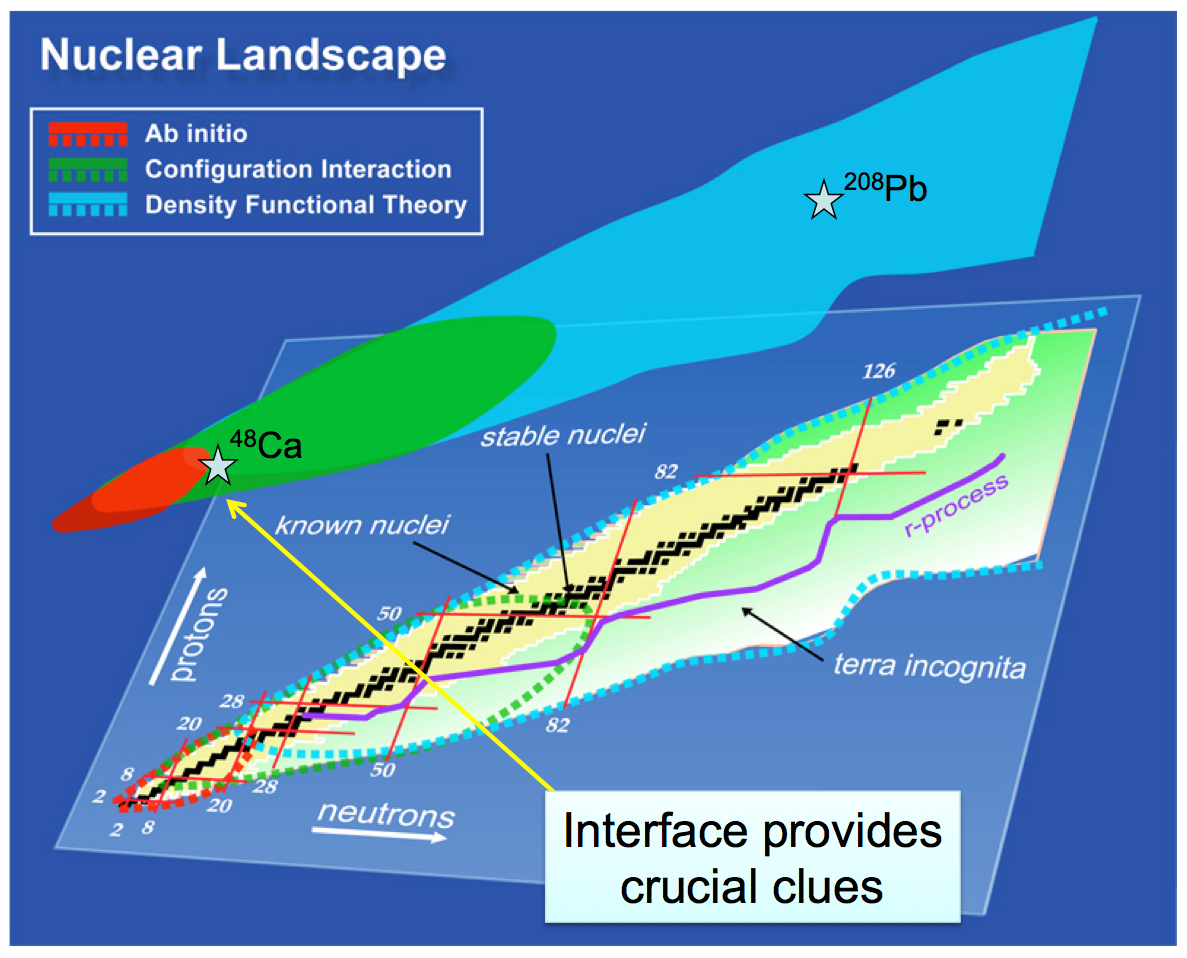
\includegraphics[width=0.5\linewidth]{Nuclear_Landscape}
\end{figure}

%%%%%%%%%%%%%%%%%%%%%%%%%%%%%%%%%%%%%%%%%%%%%%%%
\subsection{Physical Implication}

%%%%%%%%%%%%%%%%%%%%%%%%%%%%%%%%%%%%%%%%%%%%%%%%%%%%%%%%%%%%%%%%%%%%%%%%
\section{Experimental Setup}
The 2 sister experiments were carried out in Hall A of Jlab, 

% table of beam parameters
\begin{table}[h]
    \centering
    \begin{tabular}{c | c c }
	\hline
	&   PREX-II & CREX  \\
	\hline
	Target	& \Pb	& \Ca	\\
	Target thickness (mm)	& 0.5	& 6	\\
	\hline
	Beam Energy ($GeV$) & 0.97 & 2.18  \\
	Beam Current ($\mu A$)	& 70	& 150	\\
	Beam Polarization & 88\%   & 87.1\%   \\
	Scattering angle ($\deg$)   & 5	& 4.51 \\
	$Q^2$ ($GeV^2$)	&   & 0.0297	\\
	Helicity rate (Hz)  & 240   & 120   \\
	rate/arm (MHz)	&   & 25    \\
	\hline
    \end{tabular}
\end{table}

%%%%%%%%%%%%%%%%%%%%%%%%%%%%%%%%%%%%%%%%%%%%%%%%
\subsection{Design}
Though weak charge distribution is what we want to measure, it doesn't mean we
know nothing about it. Due to the symmetry between proton and neutron, we would
expect the weak charge (neutron) distribution is similar to the charge (proton)
distribution. Based on this assumption, we will have some models to describe
the neutron distribution and therefore the FFs, from which we can derive the
cross section and their asymmetry.

For symmetric nuclei with equal number of proton and neutron, it is expected 
that their density distributions are similar to each other, which are usually
expressed as a 2-parameter Fermi function:
\begin{equation}
    \rho(r) = \frac{\rho_0}{1 + exp(r-a)/c}
\end{equation}
where a and c denote the half-height radius and diffuseness respectively. 
% Thiel et al J.Phys.G 46 (2019) 9, 093003 

\subsubsection{Sensitivity}

%%%%%%%%%%%%%%%%%%%%%%%%%%%%%%%%%%%%%%%%%%%%%%%%
\subsection{Continuous Electron Beam Accelerator Facility (CEBAF)}
\begin{figure}
    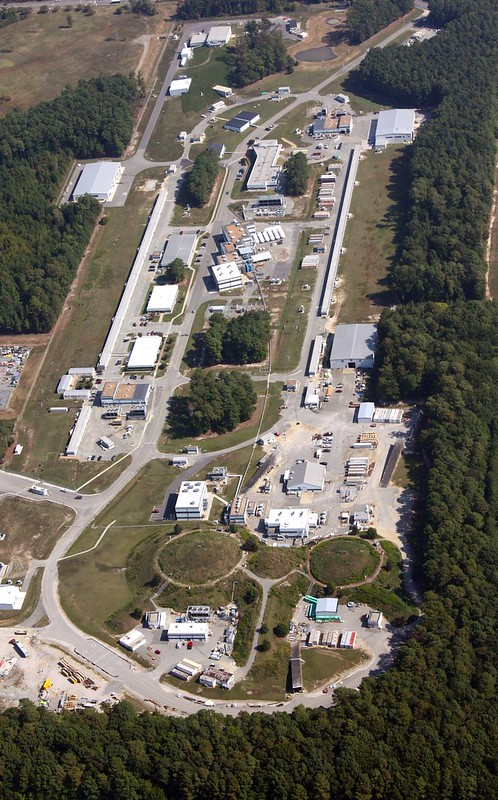
\includegraphics[width=0.44\linewidth]{jlab_1.jpg}
    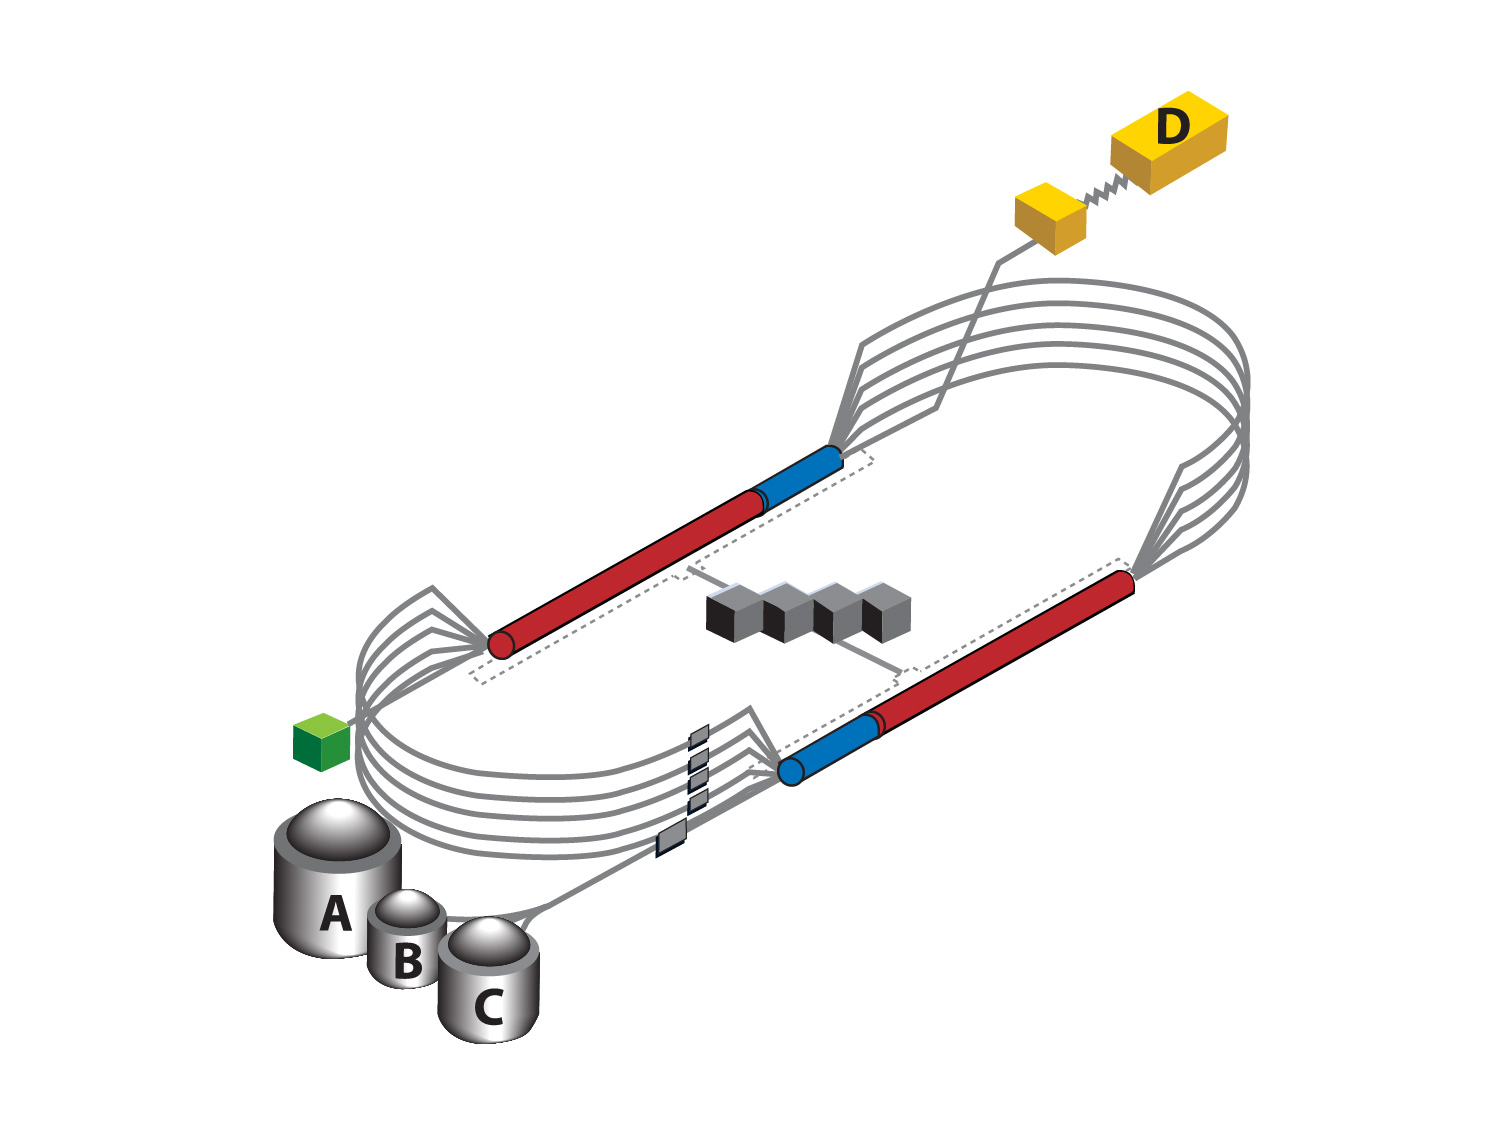
\includegraphics[width=0.8\linewidth]{cebaf}
\end{figure}
With the 12 GeV upgrade, the north and south LINAC each has 25 cryomodules, 
capable of accelrating electrons at the rate of 2.2 $GeV/turn$. The total power
of CEBAF (1 MW) limits the available beam current. For PREX-II (CREX), 
the beam current was 70 (150) $\mu A$ respectively.

%%%%%%%%%%%%%%%%%%%%%%%%%%%%%%%%%%%%%%%%%%%%%%%%
\subsection{Polarized Source}

%%%%%%%%%%%%%%%%%%%%%%%%%%%%%%%%%%%%%%%%%%%%%%%%
\subsection{Polarization Control}

%%%%%%%%%%%%%%%%%%%%%%%%%%%%%%%%%%%%%%%%%%%%%%%%
\subsection{Beam Modulation}

%%%%%%%%%%%%%%%%%%%%%%%%%%%%%%%%%%%%%%%%%%%%%%%%
\subsection{Target}

%%%%%%%%%%%%%%%%%%%%%%%%%%%%%%%%%%%%%%%%%%%%%%%%
\subsection{Magnets}

%%%%%%%%%%%%%%%%%%%%%%%%%%%%%%%%%%%%%%%%%%%%%%%%
\subsection{HRS}

%%%%%%%%%%%%%%%%%%%%%%%%%%%%%%%%%%%%%%%%%%%%%%%%
\subsection{Detector}

\chapter{Data Analysis}
As mentioned before, though of fast flipping and tremendous effort to keep electron beam in exactly
the same conditions (intensity, energy, position and angle on target) through 
opposite helicity states, life is not easy and there is no way to achieve such
a goal, after all, no one can understand completely and control every aspect of
something as complicated as an accelerator. There is always various noise caused
in various parts of the machine, though very small in general sense, they are
large compare to what we want to measure, and actually the largest correction
to PV asymmetry. So we need to remove such noise in the raw asymmetry we measured.

We use the same methods to process both PREX-II and CREX data, therefore we will
talk about only CREX data here.

\begin{table}
    \begin{tabular}{c | c c c c }
	\hline
	variable    & quadruplet    & minirun	& run	& slug	\\
	\hline
	count	    &	&   &	&   \\
	raw asymmetry ($ppk$)	&   \\
	corrected asymmetry ($ppk$)	&   \\
	\hline
	bpm4aX	\\
	bpm4aY	\\
	bpm4eX	\\
	bpm4eY	\\
	bpm12X	\\
	\hline
    \end{tabular}
    \caption{CREX Data Set}
\end{table}

\begin{table}
    \begin{tabular}{c | c c c}
	\hline
	variable    & regression    & dithering	    & Lagrangian    \\
	\hline
	slope	\\
	correction ($ppm$)  \\
	\hline
    \end{tabular}
\end{table}

CREX started commissioning around December 2019, we took the first good run on 
Dec 12. 6 slugs (slug 100 - 105) were collected before the Christmas. After 
the Christmas break, data taking was resumed until Jan 18 2020 when the \Ca 
target was damaged accidently. It tooks 5 days to prepare a new \Ca target.
Things moving on quite smoothly, we had 2 days of transverse asymmetry 
measurement from Feb 10 to Feb 12. We were a little over halfway on data taking 
when Covid-19 hitted and the lab was shut down at the end of March 2020. Fortunately,
things came back 4 months later, we had the chance to continue data taking for
about 1 month. The experiment stopped data taking on Sep 18 2020. A total charge
of 480 C was collected, among which 380 C was good charge. The dataset was clearly
seperated into 3 parts: before AT, after AT (before Covid) and after Covid, which
we will talk about later.
\begin{figure}[h!]
    \begin{tikzpicture}
	\begin{scope}
	    \node[anchor=south west, inner sep=0] (image) at (0, 0)
	    {   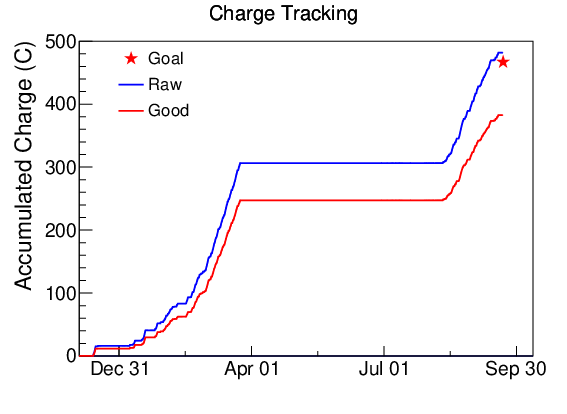
\includegraphics[width=0.45\linewidth]{charge_vs_time}
		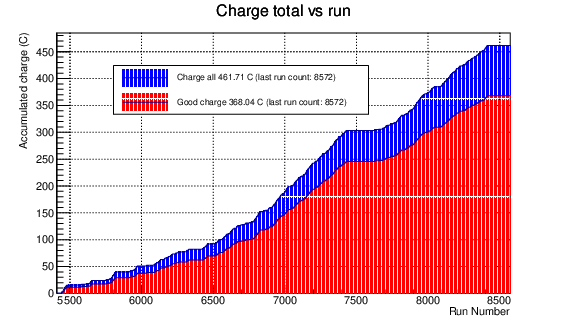
\includegraphics[width=0.54\linewidth]{charge_vs_run} };
	    \begin{scope}[x={(image.south east)},y={(image.north west)}]
		\node [Violet] at (0.3, 0.8) {Covid-shutdown};
		\draw [-stealth, Violet, line width=1pt] (0.3, 0.8) -- (0.3, 0.6);
		\node [Violet] at (0.2, 0.65) {AT};
		\draw [-stealth, Violet, line width=1pt] (0.2, 0.65) -- (0.2, 0.3);
	    \end{scope}
	\end{scope}
    \end{tikzpicture}
    \caption{Charge accumulation versus time (left) and run number (right). The
    long plateau on the left plot is due to Covid shutdown, which is shown around
    run 7500 on the right plot. We see that data taking is most efficient after
    AT (before Covid), the last month (after Covid) is not bad while the 
    first 2 months is not so efficient due to various problems.}
\end{figure}

CREX collected 1451 production runs, among them, 1386 were identified as `Good'
and used for final analysis. The good runs consists of 1362 both arms runs,
6 left arm runs and 18 right arm runs. Each good production run took about $1\ hour$
and collected about $0.3\ C$ charge with a charge efficiency of 80\%.
\begin{figure}[h!]
    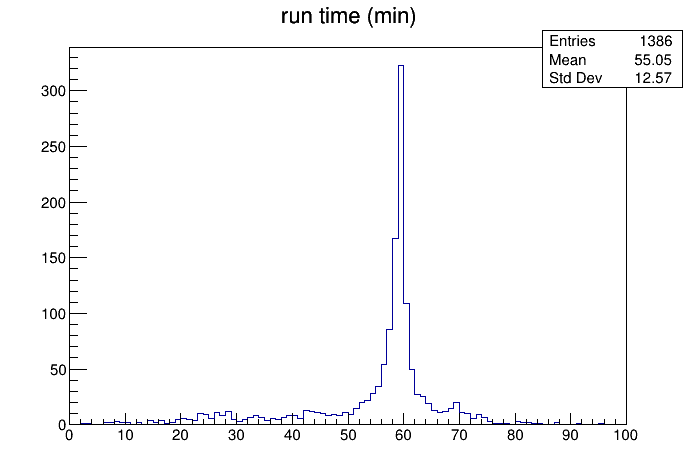
\includegraphics[width=0.32\linewidth]{crex_run_time}
    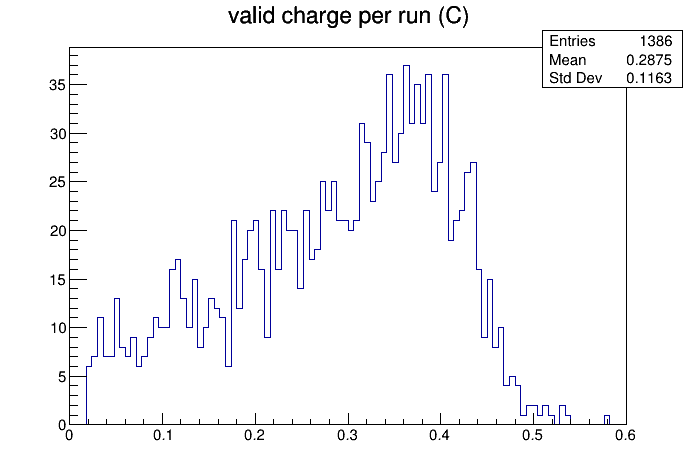
\includegraphics[width=0.32\linewidth]{crex_run_charge}
    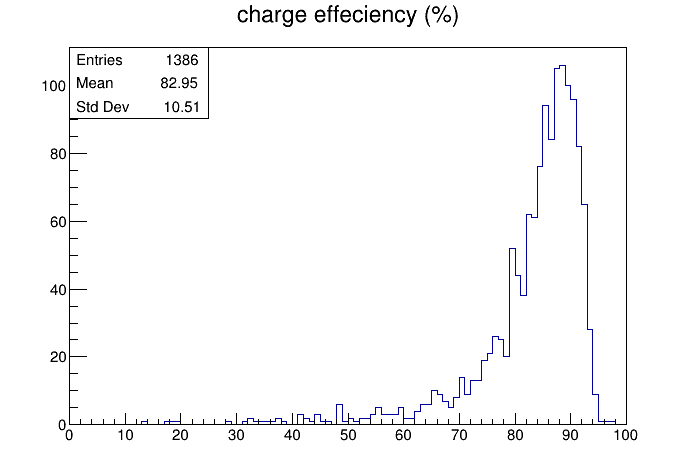
\includegraphics[width=0.32\linewidth]{crex_run_charge_efficiency}
    \caption{Statistics of CREX runs}
\end{figure}

Though electrons come bunch by bunch, the bunch frequency of $249.5\ MHz$ is much
larger than our helicity frequency of $120\ Hz$, so electron beam can be regarded
as continous. All electrons within one helicity window will be integrated as 1
record. Every 4 continuous helicty window data is grouped as quadruplet 
in order to cancel the $60\ Hz$ noise in line power, and asymmetry will be 
calculated based on quadruplet -- this is what we called one asymmetry event.
So the asymmetry event frequency is $30\ Hz$. CREX collects ??? such good 
asymmetry events.

Every run is seperated into multiple miniruns to account for the fact beam
conditions is changing quickly, it is inappropriate to calculate slope values
over a 60 mins run. Minirun will be more proper, the beam conditions, and therefore
the slope value should be more stable during such a shorter time period.  
Every minirun contains 9000 events (5 mins), the last minirun contains 
whatever number of events that can't be divided into 2 miniruns. 
CREX has 8527 miniruns in total.

Runs will be grouped into slugs. One slug is defined as all runs before the next
IHWP flipping. With good beam conditions, we could collect 3 slugs per day, so 
each slug took about 8 hours or longer in case of any accidents. CREX collects
120 slugs.

Finnaly, slugs will be grouped into part, with different wien flip status. We
have 3 parts as said before.
\begin{figure}
    \centering
    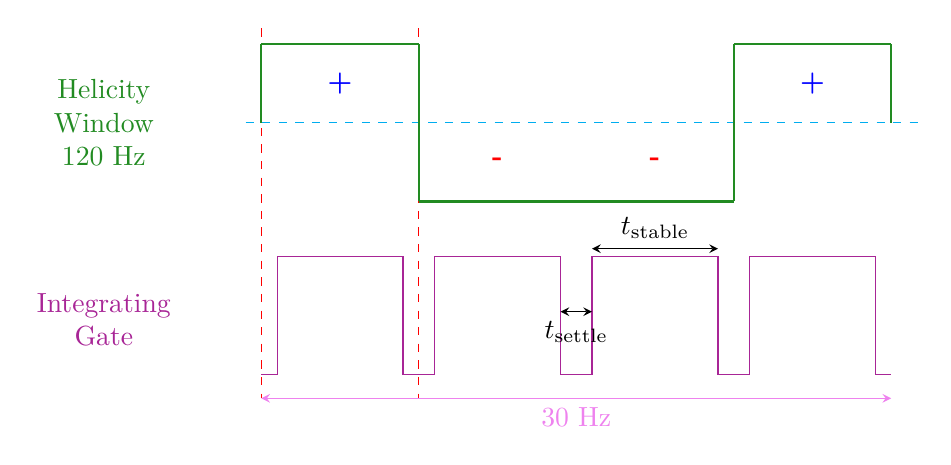
\begin{tikzpicture}[xscale=2]
	\tikzstyle{message} = [align = center]
	\draw[dashed, cyan] (-0.1, 0) -- (4.2, 0);
	\foreach \x in {0, 1}
	{ \draw[dashed, red] (\x, 1.2) -- (\x, -3.5); }
	\foreach \x in {0, 4}
	{ \draw[thick, ForestGreen] (\x, 0) -- (\x, 1); }
	\foreach \x in {1, 3}
	{ \draw[thick, ForestGreen] (\x, -1) -- (\x, 1); }
	\foreach \x in {0, 3}
	{ 
	    \draw[thick, ForestGreen] (\x, 1) -- +(1, 0); 
	    \node[blue] at (\x+0.5, 0.5) {\textbf{+}};
	}
	\foreach \x in {1, 2}
	{ 
	    \draw[thick, ForestGreen] (\x, -1) -- +(1, 0); 
	    \node[red] at (\x+0.5, -0.5) {\textbf{-}};
	}
	\node[message, ForestGreen, very thick] at (-1, 0) {Helicity \\  Window \\ 120 Hz};

	\foreach \x in {0, ..., 3}
	{
	    \draw[Mulberry] (\x, -3.2) -- ++(0.1, 0) -- ++(0, 1.5) -- ++(0.8, 0) 
	    -- ++(0, -1.5) -- ++(0.1, 0);
	}
	\draw[stealth-stealth, black] (2.1, -1.6) -- node[above] {$t_{\text{stable}}$}+(0.8, 0) ;
	\draw[stealth-stealth, black] (1.9, -2.4) -- node[below] {$t_{\text{settle}}$}+(0.2, 0) ;
	\draw[stealth-stealth, Violet] (0, -3.5) -- node[below] {30 Hz} +(4, 0);
	\node[message, Mulberry, very thick] at (-1, -2.5) {Integrating \\ Gate};
    \end{tikzpicture}
    \caption{For CREX, $t_{\text{settle}} = 90\ \mu s$, to allow the PC stablizes
    after flipping, avoiding any cross effect from last helicity state. The 
    deputy factor is 98.92\%.}
\end{figure}

%%%%%%%%%%%%%%%%%%%%%%%%
\subsubsection{Cut}
We have only very loose cut on datas to keep as much data as possible. The online
cuts include a current cut and some stability cuts. The current cut requires
the beam current no smaller than $15\ \mu A$ below the nominal current, due to 
non-linearity in monitor/detector pedestals. The stability cut says ???
%%%%%%%%%%%%%%%%%%%%%%%%
\subsubsection{Beam Current}
We have 5 bcms and the upstream analog bcm is used as the target current monitor.
where are the 5 bcms
why choose bcm\_an\_us as bcm\_target?

\begin{itemize}
    \item non-linearity from electronics read out: false asymmetry. PMT $\rightarrow$
	preamplifier $\rightarrow$ ADC
\end{itemize}

Data quality:
\begin{itemize}
    \item Beam excursion: data quality cuts are applied to remove unstable beam periods
	FIXME: a plot for beam excursion
\end{itemize}

%%%%%%%%%%%%%%%%%%%%%%%%%%%%%%%%%%%%%%%%%%%%%%%%%%%%%%%%%%%%%%%%%%%%%%%%
\section{Raw Data}
What we call one event is all electrons counted in one helicity window.
The asymmetry value is calculated using every 4 (8 in PREX-II) helicity windows
(+\-\-+ or -++-)to cancel the 60 Hz line power noise. The helicity pattern was
chosed pseduo-randomly. The CREX data consists of ??? event.

ErrorFlag 

beam jetter ??? in position, ??? in energy and ??? in time scale

Every event
is accompanied by a set of beam parameter values, recording the beam conditions
in that helicity window. A series of cut will be applied, basing on the beam
stability, to select good charge.

\subsubsection{Pair value}
For any 2 continuous events, define their pair value as:
For BPM/BCM, the pair difference is:
$$ diff = \frac{v^+ - v^-}{2} $$

For usl/usr, the asymmetry is:
$$ asym = \frac{v^+ - v^-}{v^+ + v^-} $$

\subsection{Measured Asymmetry}
\subsection{Beam False Asymmetry}

Can we count number of electrons from detector read out?

%%%%%%%%%%%%%%%%%%%%%%%%%%%%%%%%%%%%%%%%%%%%%%%%%%%%%%%%%%%%%%%%%%%%%%%%
\section{Regression}

\subsection{The Model}
Considering one monitor and one detector. Assuming the reading noise of detector
follows the Gaussian distribution and the monitor is precise:
\begin{equation*}
    \begin{gathered}
	M = m	\\
	D = d + \epsilon(0, \sigma_0^D)    \\
    \end{gathered}
\end{equation*}
Here, M (D) is the measured value while m (d) is the true value and $\sigma_0^D$ 
is the variance of the noise for Detector.

Then the difference between beams of opposite polarization will follow also
the Gaussian distribution with a larger variance:
\begin{equation*}
    \begin{gathered}
	\Delta M = M^+ - M^- = d^+ - d^-    
	    = \Delta d_0    \\
	\Delta D = D^+ - D^- = (d^+ + \epsilon(0, \sigma_0^D)) - (d^- + \epsilon(0, \sigma_0^D))
	    = \Delta d_0 + \epsilon(0, \sqrt{2}\sigma_0^D)
	    = \Delta d_0 + \epsilon(0, \sigma_1^D) \\
    \end{gathered}
\end{equation*}
Again, $\Delta m_0$ ($\Delta d_0$) is the real difference between the
different polarized beams while $\Delta M$ ($\Delta D$) is the measured value.

The probability for measuring $\Delta D$ will be:
\begin{equation*}
    \begin{gathered}
	P(\Delta D) = \frac{1}{\sigma_1^D\sqrt{2\pi}} e^{-\frac{1}{2}\left( \frac{\Delta D - \Delta d_0}{\sigma_1^D}\right)^2}    \\
    \end{gathered}
\end{equation*}

We will have a bunch of data points: $(\Delta M, \Delta D)_i$ and we want to
extract the relationship between $\Delta d_0$ and $\Delta m_0$: 
$c \equiv \frac{\partial d}{\partial m}$ -- given the tinyness of $\delta m$, first
order is precise enough. This is exactly a regression problem.
$$ \Delta d = c \Delta m $$

For any real data point $(\Delta m_0, \Delta d_0)_i$, the possibility to measure
$(\Delta M, \Delta D)_i$ is:
\begin{equation*}
    \begin{gathered}
	P_i(\Delta D|\Delta M) = \frac{1}{\sigma_1^D\sqrt{2\pi}} 
	    e^{-\frac{1}{2}\left( \frac{\Delta D - c\Delta m_0}{\sigma_1^D}\right)^2}
    \end{gathered}
\end{equation*}

For the accumulated data of one minirun, the total probability will be:
\begin{equation*}
    P = \prod_i^n P_i(\Delta D|\Delta M) = \prod_i^n \frac{1}{\sigma_1^D\sqrt{2\pi}} 
	    e^{-\frac{1}{2}\left( \frac{\Delta D_i - c\Delta m_0}{\sigma_1^D}\right)^2}
\end{equation*}

What's the typical noise of bcm/bpm?


%%%%%%%%%%%%%%%%%%%%%%%%%%%%%%%%%%%%%%%%%%%%%%%%%%%%%%%%%%%%%%%%%%%%%%%%
\section{Beam Modulation}

%%%%%%%%%%%%%%%%%%%%%%%%%%%%%%%%%%%%%%%%%%%%%%%%%%%%%%%%%%%%%%%%%%%%%%%%
\section{Lagragian}

%%%%%%%%%%%%%%%%%%%%%%%%%%%%%%%%%%%%%%%%%%%%%%%%%%%%%%%%%%%%%%%%%%%%%%%%
\section{Correction}
\begin{itemize}
    \item background dilution
\end{itemize}
%%%%%%%%%%%%%%%%%%%%%%%%%%%%%%%%%%%%%%%%%%%%%%%%%%%%%%%%%%%%%%%%%%%%%%%%
\section{Result}

\chapter{Transverse Asymmetry}
The Beam Normal Single Spin Asymmetry (BNSSA, also known as Transverse Single Spin Asymmetry
or Transverse Asymmetry) is different from the PV asymmetry, it is purely 
electromagnetic and therefore parity-conserving. It arises from the interference
between one-photon and two-photon exchange (OPE and TPE), therefore it is sensitive 
to the TPE amplitude. By measuring it, we can probe the strength of TPE, an 
important knowledge of electron elastic scattering that may explain the myth
of proton radius measured with different methods.

The transverse asymmetry is also an important systematic uncertainty to our PV 
asymmetry measurement, because there is always some residual transverse polarization
in the electron beam. With $\CA_n \sim \alpha_{EM}m_e/E_e$, its magnitude of $10^{-5}$
for a GeV level electron beam is much larger than $\CA_{pv}$, so a complete 
understanding and precise measurement of the transverse asymmetry is needed
to ensure accurate correction of $\CA_{pv}$.

Being a routine and bonus of a PV experiment, PREX-I also measured the transverse
asymmetry of some nuclei, namely ${}^{1}H$, \He, \C and \Pb. Surprisingly, PREX-I
saw a zero transverse asymmetry in \Pb, while the transverse asymmetries of other 
light nuclei seemed to agree with theoretical predictions, as shown in 
Fig. \ref{fig:PREX-I_AT}. One of the reason for PREX-II was that we wanted to
verify the zero measurement in \Pb, which remains as a challenge to theorists.
\begin{figure}
    \centering
    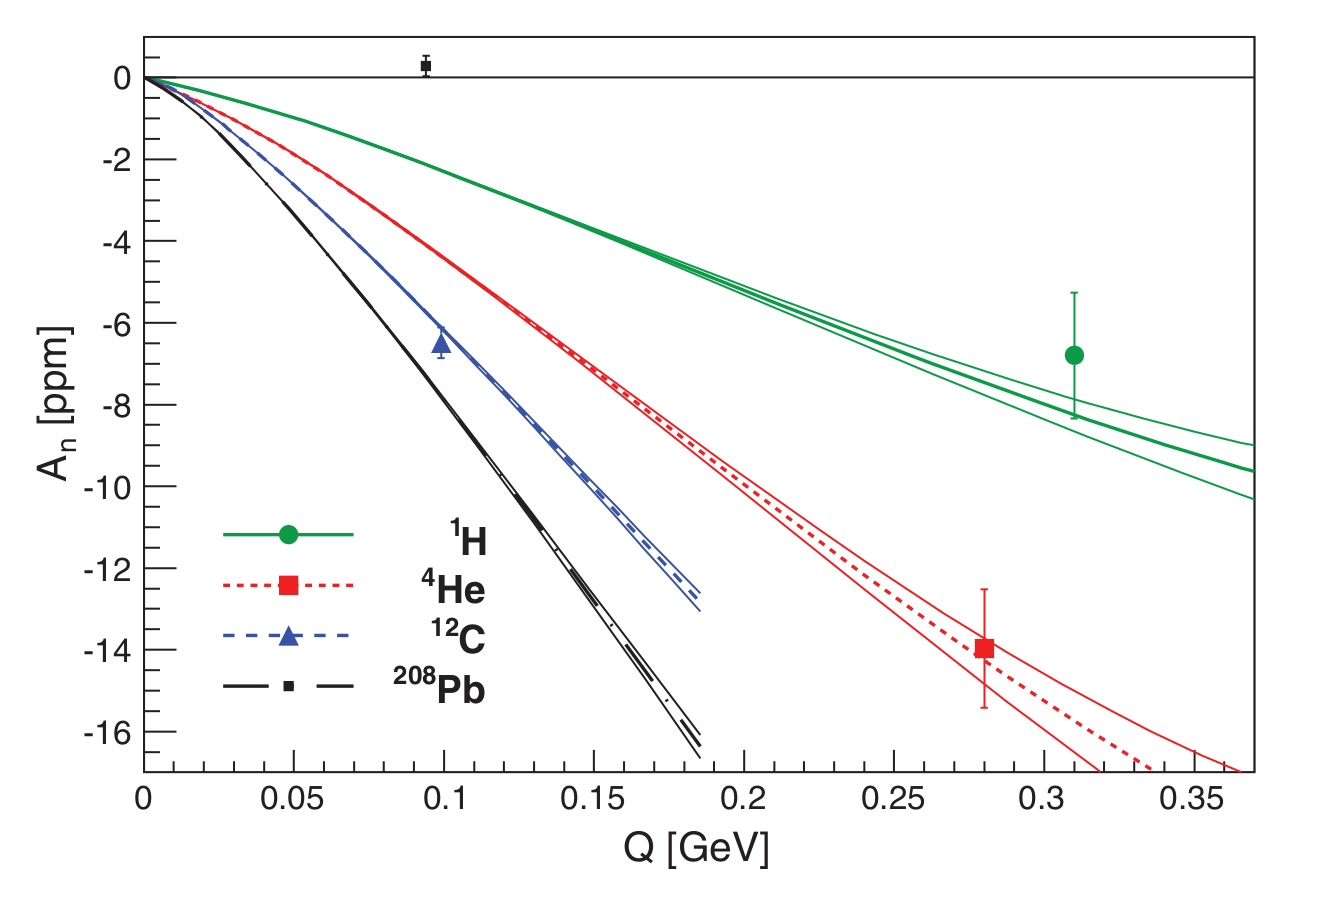
\includegraphics[width=0.5\linewidth]{PREX-I_AT}
    \caption{Transverse asymmetry measured in PREX-I.}
    \label{fig:PREX-I_AT}
\end{figure}

As its name implies, BNSSA depends on only one spin, either the target or the
electron, polarized target is better that polarized target in that it is hard
to polarize nuclei, especially heavy nuclei.

%%%%%%%%%%%%%%%%%%%%%%%%%%%%%%%%%%%%%%%%%%%%%%%%%%%%%%%%%%%%%%%%%%%%%%%%
\section{Motivation for Transverse Asymmetry}

%%%%%%%%%%%%%%%%%%%%%%%%
\subsubsection{The Scattering Theory}
Consider the scattering of a free ($t_0 \rightarrow -\infty$) particle from a 
time independent potential $V(\vec{r})$, 
which decays quickly as $r \rightarrow \infty$. The evolution from the free initial state
$\ket{i}$ is denoted as $\ket{\psi(t)}_S$ (under the Schr\"odinger picture, $\hbar = 1$):
\begin{equation}
    \ket{\psi(t)}_S = U(t)\ket{\psi(t_0)} = \lim_{t_0 \rightarrow -\infty}U(t, t_0)\ket{i}
\end{equation}
where $U(t, t_0)$ is the evolution operator:
\begin{equation}
    U(t, t_0) = \exp(\frac{1}{i}(H_0 + V)(t - t_0)) = \exp(-i(H_0 + V)(t-t_0))
\end{equation}
$H_0$ is the free Hamiltonian and $H = H_0 + V$ is the complete Hamiltonian
with interaction term. 

The projection of $\psi(t)$ to a free final state $\ket{f}$ defines the so called
S-matrix (the order of the subscripts matters):
\begin{equation}
    S_{if} \equiv \lim_{t\rightarrow +\infty}\bra{f}\ket{\psi(t)} 
    = \lim_{t\rightarrow\infty} \lim_{t_0 \rightarrow -\infty} \bra{f} U(t, t_0) \ket{i}
\end{equation}
Which defines the S operator:
\begin{equation}
    S_{if} = \bra{f} S \ket{i} \Longrightarrow S = U(+\infty, -\infty)
\end{equation}

The S-matrix describe the scattering amplitude from the free initial state $\ket{i}$
to the free final state $\ket{f}$. Conservation of probability indicates
unitary of S matrix:
\begin{equation}
    S^\dag S = \sum_f |\bra{f} U(+\infty, -\infty) \ket{i}|^2 = 1
\end{equation}

It is easier to evaluate $U(t)$ in the interaction picture. Define
\begin{equation}
    \ket{\psi(t)}_I \equiv \exp(-\frac{1}{i}H_0 t) \ket{\psi(t)}_S 
    = \exp(iH_0 t) \exp(-i (H_0 + V) t)\ket{i}
\end{equation}
The subscript I and S denote the interaction and Schr\"odinger picture respectively.
The evolution of $\ket{\psi(t)}_I$ is:
\begin{equation}
    \begin{aligned}
	\frac{d}{dt}\ket{\psi(t)}_I 
	&= \left[ \exp(i H_0 t) (iH_0) \exp(-i (H_0 + V) t)
	+ \exp(i H_0 t) (-i)(H_0 + V) \exp(-i (H_0 + V) t) \right] \ \ket{i}  \\
	&= -i\ \exp(i H_0 t)\ V \ \exp(-i (H_0 + V) t) \ket{i}   \\
	&= -i \exp(iH_0 t) V \exp(-iH_0 t) \cdot \exp(iH_0 t) \exp(-i(H_0 + V)t) \ket{i}   \\
	&= -i V_I(t) \ket{\psi(t)}_I
    \end{aligned}
    \label{eq:interaction_evolution}
\end{equation}
where $V_I(t) = \exp(iH_0t)V\exp(-iH_0t)$ is the time dependent interaction term.
Eq. \ref{eq:interaction_evolution} leads to the Dyson series:
\begin{equation}
    U(t, t_0) = 1 - i\int_{t_0}^t dt_1 V_I(t_1) U(t_1, t_0) = \sum_{n=0}^\infty \frac{(-i)^n}{n!}\int_{t_0}^t dt_1 \cdots \int_{t_0}^t dt_n T[V_I(t_1)\cdots V_I(t_n)]
\end{equation}
T means time-ordering:
\begin{equation}
    T(V_I(t_1) V_I(t_2)) \equiv 
    \begin{cases}
	V_I(t_1)V_I(t_2)    & t_1 \le t_2   \\
	V_I(t_2)V_I(t_1)    & t_2 \le t_1   \\
    \end{cases}
\end{equation}

\begin{equation}
    \begin{aligned}
	\bra{f} U(t, t_0) \ket{i} 
	&= \bra{f}\ket{i} - i \bra{f} \int_{t_0}^t dt_1 V_I(t_1) U(t_1, t_0) \ket{i}	\\
	&= \delta_{if} - i\sum_m \int_{t_0}^t dt_1 \bra{f}\exp(iH_0 t_1) V \exp(-iH_0 t_1)(t_1)\ket{m} \bra{m} U(t_1, t_0) \ket{i} \\
	&= \delta_{if} - i\sum_m \bra{f}V\ket{m} \int_{t_0}^t dt_1 \exp(i(E_f - E_m)t_1) \bra{m}U(t_1, t_0)\ket{i}  \\
    \end{aligned}
    \label{eq:finite_S-matrix}
\end{equation}
Truncate Eq. \ref{eq:finite_S-matrix} into first order ($\bra{m} U(t_1, t_0) \ket{i} = \delta_{im}$)
and define $T_{if} = \bra{f} V \ket{i}$, we will get:
\begin{equation}
    \bra{f} U(t, t_0) \ket{i} = \delta_{if} - iT_{if} \int_{t_0}^t dt_1 \exp(i(E_f - E_i)t_1)
\end{equation}
and 
\begin{equation}
    \begin{aligned}
	S_{if} &= \lim_{t\rightarrow +\infty}\lim_{t_0 \rightarrow -\infty} \bra{f} U(t, t_0) \ket{i}    \\
	    &= \delta_{if} - iT_{if} \int_{-\infty}^{\infty} dt_1 \exp(i(E_f - E_i)t_1)	\\
	    &= \delta_{if} + i2\pi\delta(E_f - E_i)T_{if}   \\
    \end{aligned}
\end{equation}
In matrix form:
\begin{equation}
    S = 1 + i2\pi T
\end{equation}
S begin unitary implies
\begin{equation}
    S^\dag S = (1 - i2\pi T^\dag) (1 + i2\pi T) = 1 + i2\pi(T - T^\dag) + (2\pi)^2 T^\dag T = 1
\end{equation}
which reads
\begin{equation}
    T - T^\dag = i (2\pi)T^\dag T = i(2\pi) T T^\dag
\end{equation}
In terms of matrix element:
\begin{equation}
    \begin{gathered}
    \delta(E_f - E_i)(T_{if} - T^\dag_{if}) = \sum_m i2\pi\delta(E_f - E_m)\delta(E_m - E_i)T_{fm}T^\dag_{mi}	\\
    T_{if} - T^\dag_{if} = \sum_m i2\pi\delta(E_m - E_i)T_{fm}T^\dag_{mi} = ia_{if} \\
    \end{gathered}
\end{equation}
where 
\begin{equation}
    a_{if} = \sum_m (2\pi) \delta(E_m - E_i)T_{fm}T^\dag_{mi}
\end{equation}
is the absorptive part of the transition amplitude $T_{if}$. $\ket{m}$ extends
to all on-shell intermediate states.

The two parts of S are easy to understand.
The constant piece denotes the evolution of one free particle into another free
particle without any interactions; obviously, it can evolve only into itself.
The T matrix describe the interaction (transition amplitude) between the free
initial particle $\ket{i}$ and the free final particle $\ket{j}$, which tells
us the interaction cross section.

The free particle state can be completely described by its momentum (ignoring spin
for now) $\vec{p}$. For an incoming electron $\ket{\vec{p}_i}$, the probability
to transform into the final state of $\ket{\vec{p}_f}$ is:
\begin{equation}
    dP = (phase\ space) \times (transition\ probability) = \frac{d\vec{p}_f}{(2\pi)^3} \times |S_{\vec{p}_i\vec{p}_f}|^2
\end{equation}
For a non trivial case of $\ket{f} \ne \ket{i}$, we have:
\begin{equation}
    S_{if} = i2\pi \delta(E_f - E_i)T_{if}
\end{equation}
The differential cross section will be:
\begin{equation}
    d\sigma = \frac{dP}{\CL \Delta t}
\end{equation}
where $\CL$ is the luminosity, indicating number of particles hitting 
the target per unit area per unit time, in our case of incoming plane wave, 
$\CL = \rho v = v$, and $\Delta t$ is the interaction time.
\begin{equation}
    d\sigma = \frac{1}{v\Delta t} \frac{d\vec{p}_f}{(2\pi)^3} 2\pi\delta(E_f - E_i) \left. 2\pi\delta(E_f - E_i)\right|_{E_f = E_i} |T_{if}|^2
\end{equation}
Transform one $\delta$ back to integrating form: 
\begin{equation}
    \left. 2\pi\delta(E_f - E_i) \right|_{E_f = E_i} 
    = \int_{-\infty}^{+\infty} dt \left.\exp(-i(E_f - E_i)t)\right|_{E_f = E_i}
    = \int_{-\infty}^{+\infty} dt 
\end{equation}
Physically, we don't go back or into infinity in time, because the real particle
is a finite wave packet rather than a plane wave. The integration above should 
be finite and close to the interaction time
\begin{equation}
    \int_{-\infty}^{+\infty} dt \rightarrow \Delta t
\end{equation}
Thus we have a defined cross section
\begin{equation}
    d\sigma = \frac{1}{v} \frac{d\vec{p}_f}{(2\pi)^3} 2\pi\delta(E_f - E_i) |T_{if}|^2
\end{equation}
The cross section is proportional to $|T_{if}|^2$, as known to us.


%%%%%%%%%%%%%%%%%%%%%%%%
\subsubsection{T-Symmetry}
Symmetry is the most profound concept and foundation of modern physics, which
can be separated into continuous symmetries and discrete ones. Time symmetry
is one important discrete symmetry, which states that physical laws should
keep unchanged under time reversal operation. Time reversal is the operation
that flips time arrow, so that time runs backward after time reversal. Obviously, 
vectors that are first order of time derivative will also reverse sign, such
as momentum, angular momentum and magnetic field.

Express the time reversal operation in QM:
\begin{equation}
    \ket{\tilde{\psi}} = \hat{\mathcal{T}} \ket{\psi} 
\end{equation}
where $\hat{\mathcal{T}}: t \rightarrow -t$ is the time reversal operator. 

In terms of our scattering, as said above, a particle will flip its momentum 
and spin (angular momentum) under time reversal, and pick up a phase.
\begin{equation}
    \ket{\tilde{\psi}} = \hat{\mathcal{T}} \ket{\psi_\uparrow(\vec{k})} = \eta\ket{\psi_\downarrow(-\vec{k})}
\end{equation}
$\eta$ is the phase difference, $|\eta|^2 = 1$. So the T matrix can also be applied
to time reversed state
\begin{equation}
    T_{\tilde{i}\tilde{f}} = \bra{\tilde{f}} V \ket{\tilde{i}}
\end{equation}

It is well known that electromagnetic interaction is invariant under time reversal.
\begin{equation}
    |T_{if}|^2 = |T_{\tilde{f}\tilde{i}}|^2 
\end{equation}

With these concepts, one can also define the \textbf{T-odd} quantities which
are proportional to the difference of the magnitude of a normal T element and 
its half time reversed version:
\begin{equation}
    \begin{aligned}
	\text{T-odd} &\propto |T_{if}|^2 - |T_{\tilde{i}\tilde{f}}|^2	\\
	    &= |T_{if}|^2 - |T_{fi}|^2	\\
	    &= |T_{if}|^2 - |T^\dag_{if}|^2	\\
	    &= |T_{if}|^2 - |T_{if} - ia_{if}|^2	\\
	    &= -i(T_{if}a^*_{if} - T^*_{if}a_{if}) - |a_{if}|^2	\\
	    &= 2Im(T_{if}a^*_{if}) - |a_{if}|^2
    \end{aligned}
    \label{eq:T-odd}
\end{equation}

%%%%%%%%%%%%%%%%%%%%%%%%
\subsubsection{Transverse Asymmetry}
Denote the incoming and outgoing transversely polarized electrons as 
$\ket{\vec{k}}$ and $\ket{\vec{k}'}$, the scattering is shown in Fig. \ref{fig:transverse_scattering}.
\begin{figure}[h!]
    \centering
    \begin{subfigure}[c]{0.4\linewidth}
	\begin{tikzpicture}[scale=0.8]
	    \begin{feynman}[transform shape]
		\vertex (i1) {$e^-$};
		\vertex [right=1.0cm of i1, inner sep=0pt] (spin) {$\odot$};
		\vertex [right=2.3cm of spin] (ip);
		\vertex [right=2.8cm of ip] (i2) {A};
		\vertex [above right = 2cm and 2cm of ip] (o1) {$e^-$};
		\vertex [below left = 2cm and 2cm of ip] (o2) {A};

		\diagram* { {[edge=fermion]
		    (spin) --[edge label=$\vec{k}$] (ip) [dot] --[edge label = $\vec{k}'$] (o1),
		    (i2) --[edge label=$\vec{p}$](ip) [dot] -- [edge label = $\vec{p}'$]  (o2)},
		    (i1) -- (spin)
		};
	    \end{feynman}
	\end{tikzpicture}
    \end{subfigure}
    \hspace{0.2 cm}
    \textbf{-}
    \hspace{0.5 cm}
    \begin{subfigure}[c]{0.4\linewidth}
	\begin{tikzpicture}[scale=0.8]
	    \begin{feynman}[transform shape]
		\vertex (i1) {$e^-$};
		\vertex [right=1.0cm of i1, inner sep=0pt] (spin) {$\otimes$};
		\vertex [right=2.3cm of spin] (ip);
		\vertex [right=2.8cm of ip] (i2) {A};
		\vertex [above right = 2cm and 2cm of ip] (o1) {$e^-$};
		\vertex [below left = 2cm and 2cm of ip] (o2) {A};

		\diagram* { {[edge=fermion]
		    (spin) --[edge label=$\vec{k}$] (ip) [dot] --[edge label = $\vec{k}'$] (o1),
		    (i2) --[edge label=$\vec{p}$](ip) [dot] -- [edge label = $\vec{p}'$]  (o2)},
		    (i1) -- (spin)
		};
	    \end{feynman}
	\end{tikzpicture}
    \end{subfigure}
    \caption{Feynman plots of transversely polarized electron scatters off
    unpolarized nuclear target in the CoM. } 
    \label{fig:transverse_scattering}
\end{figure}

The transverse asymmetry will be:
\begin{equation}
    \CA_n \equiv \frac{N_{\uparrow} - N_{\downarrow}}{N_{\uparrow} + N_{\downarrow}} 
    = \frac{|T_{\uparrow}(\vec{k}, \vec{k}')|^2 - |T_{\downarrow}(\vec{k}, \vec{k}')|^2}{|T_{\uparrow}(\vec{k}, \vec{k}')|^2 + |T_{\downarrow}(\vec{k}, \vec{k}')|^2}
\end{equation}
where $T(\vec{k}, \vec{k}') = \bra{\vec{k}'} V \ket{\vec{k}}$ is the scattering
amplitude and the arrow subscript indicates electron's spin direction.
$T_\downarrow(\vec{k}, \vec{k}')$ is related to $T_\downarrow(-\vec{k}, -\vec{k}')$
by a rotation around the normal direction of the scattering plane, as shown in
Fig. \ref{fig:rotation_plot}
\begin{figure}[h!]
    \centering
    \begin{subfigure}[c]{0.4\linewidth}
	\begin{tikzpicture}[scale=0.8]
	    \begin{feynman}[transform shape]
		\vertex (i1) {$e^-$};
		\vertex [right=1.0cm of i1, inner sep=0pt] (spin) {$\odot$};
		\vertex [right=2.3cm of spin] (ip);
		\vertex [right=2.8cm of ip] (i2) {A};
		\vertex [above right = 2cm and 2cm of ip] (o1) {$e^-$};
		\vertex [below left = 2cm and 2cm of ip] (o2) {A};

		\diagram* { {[edge=fermion]
		    (spin) --[edge label=$\vec{k}$] (ip) [dot] --[edge label = $\vec{k}'$] (o1),
		    (i2) --[edge label=$\vec{p}$](ip) [dot] -- [edge label = $\vec{p}'$]  (o2)},
		    (i1) -- (spin)
		};
	    \end{feynman}
	\end{tikzpicture}
    \end{subfigure}
    \hspace{0.2 cm}
    $\Longrightarrow$
    \hspace{0.5 cm}
    \begin{subfigure}[c]{0.4\linewidth}
	\begin{tikzpicture}[scale=0.8]
	    \begin{feynman}[transform shape]
		\vertex (i1) {$e^-$};
		\vertex [left=1.0cm of i1, inner sep=0pt] (spin) {$\odot$};
		\vertex [left=2.3cm of spin] (ip);
		\vertex [left=2.8cm of ip] (i2) {A};
		\vertex [below left = 2cm and 2cm of ip] (o1) {$e^-$};
		\vertex [above right = 2cm and 2cm of ip] (o2) {A};

		\diagram* { {[edge=fermion]
		    (spin) --[edge label=$\vec{k}$] (ip) [dot] --[edge label = $\vec{k}'$] (o1),
		    (i2) --[edge label=$\vec{p}$] (ip) [dot] -- [edge label = $\vec{p}'$] (o2)},
		    (i1) -- (spin)
		};
	    \end{feynman}
	\end{tikzpicture}
    \end{subfigure}
    \caption{Rotation by $\pi$ around the normal direction.} 
    \label{fig:rotation_plot}
\end{figure}
\begin{equation}
    T_\downarrow(\vec{k}, \vec{k}') = e^{i\pi} T_\downarrow(-\vec{k}, -\vec{k}')
\end{equation}

Let $T_{if} = T_{\uparrow}(\vec{k}, \vec{k}')$, then $T_{\tilde{i}\tilde{f}} = T_\downarrow (-\vec{k}, -\vec{k}')$
and
\begin{equation}
    \begin{aligned}
	\CA_n &\approx \frac{|T_{\uparrow}(\vec{k}, \vec{k}')|^2 - |T_{\downarrow}(-\vec{k}, -\vec{k}')|^2}{2|T_{\uparrow}(\vec{k}, \vec{k}')|^2} \\
	    &= \frac{|T_{if}|^2 - |T_{\tilde{i}\tilde{f}}|^2}{2|T_{if}|^2}  \\
	    &= \frac{2Im(T_{if}a^*_{if}) - |a_{if}|^2}{2|T_{if}|^2}
    \end{aligned}
    \label{eq:transverse_asymmetry}
\end{equation}

We see that the transverse asymmetry is a T-odd quantity. For EM interaction
\begin{equation}
    T_{if} \propto \alpha \qquad a_{if} \propto \alpha^2
\end{equation}
Because $\alpha \simeq \frac{1}{137}$ is small, we can expand Eq. \ref{eq:transverse_asymmetry} 
in order of $\alpha$. To the lowest order
\begin{equation}
    \CA_n = 0
    \label{eq:AT_0}
\end{equation}
and to the first order 
\begin{equation}
    \CA_n = \frac{Im(T_{if}a^*_{if})}{|T_{if}|^2}
    \label{eq:AT_1}
\end{equation}

$T_{ij}$ represents the OPE interaction while $a_{ij}$ represents
the TPE interaction. So the physical interpretation of
Eq. \ref{eq:AT_0} and \ref{eq:AT_1} is that time reversal symmetry requires 
the transverse asymmetry to be zero under the Born approximation (OPE only)
and the (lowest order) non-zero transverse asymmetry comes from the interference 
between OPE and TPE.
\begin{figure}[h!]
    \centering
    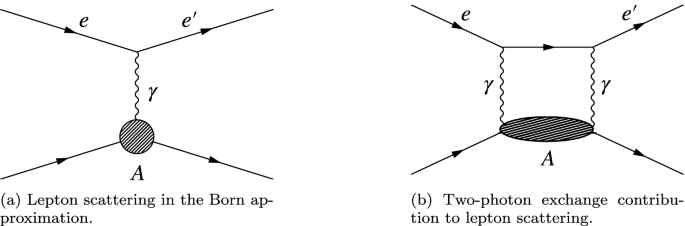
\includegraphics[width=0.8\linewidth]{at/OPE_n_TPE}
\end{figure}

%%%%%%%%%%%%%%%%%%%%%%%%%%%%%%%%%%%%%%%%%%%%%%%%%%%%%%%%%%%%%%%%%%%%%%%%
\section{How to Measure the Transverse Asymmetry: the Method}
The experimentally measured transverse asymmetry will be
\begin{equation}
    \CA_{mea} = \CA_n \vec{p}_e \cdot \hat{n} = \CA_n P_n \sin(\phi_s - \phi_e) = \CA_n P_n \sin\phi
    \label{eq:measured_AT}
\end{equation}
where $\vec{p}_e$ is the electron spin vector, whose magnitude is the polarization,
and $\phi_s$ being its angle w.r.t. the lab horizontal plane; 
$\hat{n} = \frac{\vec{k} \times \vec{k}'}{|\vec{k} \times \vec{k}'|}$ 
is the unit normal vector of the scattering plane and $\phi_e$ the angle between
the scattering plane and the lab horizontal plane. As shown in Fig. \ref{fig:AT_scattering}.
So $\phi = \phi_s - \phi_e$ is angle between the spin vector and the scattering plane.
\begin{figure}[h!]
    \centering
    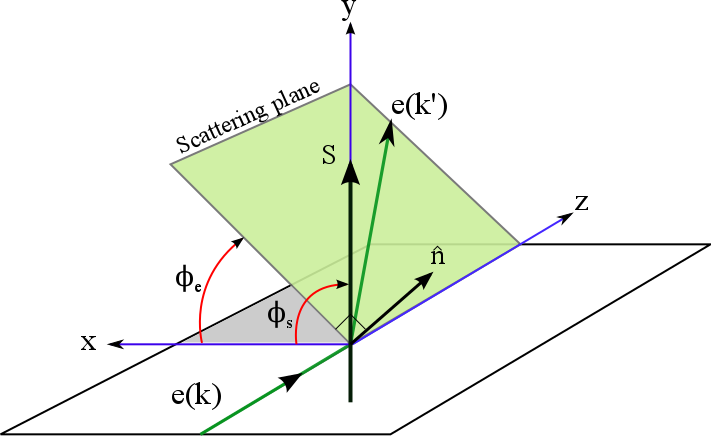
\includegraphics[width=0.7\linewidth]{AT_scattering}
    \caption{Schematic plot of scattering of transversely polarized electron.}
    \label{fig:AT_scattering}
\end{figure}

We see an angle dependence of the measured transverse asymmetry. Experimentally,
it is convenient to select the angle $\phi$ being $90^\circ$, which
usually set the lab horizontal plane as the scattering plane and the electron spin
is perpendicular to the scattering plane, as we did in PREX-II and CREX. Detailed
dynamics for AT measurement are list in Table \ref{tab:AT_dynamics}.

\begin{table}
    \centering
    \begin{tabular}{c c | c c c}
	\hline
	Exp (Energy)	& Target    & $\langle \theta \rangle ({}^\circ)$   & $\langle Q^2 \rangle \ (GeV^2)$	& $\langle \sin\phi \rangle$	\\
	\hline
	\multirow{3}{*}{PREX-II ($0.95\ GeV$)}
	    & \C    & 4.87  & 0.0067    & 0.967 \\ 
	    & \ca   & 4.81  & 0.0067    & 0.964 \\ 
	    & \Pb   & 4.69  & 0.0064    & 0.966 \\ 
	\hline
	\multirow{4}{*}{CREX ($2.18\ GeV$)}
	    & \C    & 4.77  & 0.033	& 0.969 \\ 
	    & \ca   & 4.55  & 0.031	& 0.970 \\ 
	    & \Ca   & 4.53  & 0.031     & 0.970 \\ 
	    & \Pb   & 4.60  & 0.032     & 0.969 \\ 
	\hline
    \end{tabular}
    \caption{Dynamics of AT measurement in PREX-II/CREX.}
    \label{tab:AT_dynamics}
\end{table}

To achieve transverse polarization, we needed a different configuration of the
double wien filter. Specifically, we just rotated the longitudinal spin originated
from the source to vertical direction using the vertical wien filter, the 
following rotation we did for longitudinal polarization, as shown in 
Fig. \ref{fig:double_wien_filter}, was omitted (the spin solenoid's rotating
angle was set to $~0^\circ$). Because the spin is parallel/anti-parallel
to the magnetic field in the accelerator arc, there is no spin precession as in
the case of longitudinal polarization. 

In terms of measurement of transverse polarization, neither Moller, nor Compton
polarimeter was on, because their analyzing powers go to 0 at the limit of transverse
polarization. One may wonder, if no direct measurement of polarization in the 
hall, how can we ensure the value of the polarization? Well, we had Mott measurement
in the injector, and as said above, the beam transportation from injector to Hall A
is symmetric and flat, which means the vertical component of the polarization
is preserved (can be safely assumed $>99.9\%$), so we don't need to worry about it.

Except the difference in configuration of the double wien filter, everything 
else was the same as in the case of longitudinal polarization (the Compton Chicane
was off). 

%%%%%%%%%%%%%%%%%%%%%%%%
\subsubsection{Polarization Measurement}
As said before, we don't have direct measurement of the transverse polarization
in the hall, but we verity the polarization with the Mott measurement.
The Mott polarimeter gave about 87\% polarization for both PREX-II and CREX runs.
The Mott data is summarized in Table \ref{tab:AT_Mott}.
% https://logbooks.jlab.org/entry/3781205, https://logbooks.jlab.org/entry/3718518, 
\begin{table}[!h]
    \begin{tabular}{c c c | c c | c}
	\hline
	exp & run & IHWP  & UD (\%)	& LR (\%)   & Vertical Pol (\%)	\\
	\hline
	\multirow{2}{*}{PREX-II}
	    & 8966  & OUT   & $0.0704732 \pm 0.435101$	& $-34.193 \pm 0.418556$	& -87.2048  \\
	    & 8967  & IN    & $0.421465 \pm 0.432328$	& $33.9616 \pm 0.419132$	&  86.6146  \\
	\hline
	\multirow{5}{*}{CREX}    
	    & 9081  & IN    & $-1.16128 \pm 0.334165$   & $-34.1276 \pm 0.325363$	& -87.0380  \\
	    & 9082  & OUT   & $-0.105704 \pm 0.328932$	& $34.0755 \pm 0.324116	$&  86.9051  \\
	    & 9083  & IN    & $-0.613295 \pm 0.333657$	& $-34.3502 \pm 0.32453	$& -87.6057  \\
	    & 9084  & OUT   & $-0.0248337 \pm 0.326988$	& $34.4674 \pm 0.318313	$&  87.9046  \\
	    & 9085  & IN    & $-1.15795 \pm 0.33341 $   & $-34.0401 \pm 0.32742	$& -86.8148  \\
	\hline
    \end{tabular}
    \caption{Mott measurement during PREX-II and CREX AT runnings. The Up-Down
    asymmetry measures the horizontal transverse polarization while the Left-Right
    asymmetry measures the vertical transverse polarization; The Mott analyzing 
    power is $\CA_{Mott} = 0.3921 \pm 0.0016$, so the vertical polarization is 
    $\frac{\CA_{LR}}{\CA_{mott}}$.} 
    \label{tab:AT_Mott}
\end{table}

What we used in our calculation was the average longitudinal polarization 
measured shortly before and after the AT runs, with confidence in our pretty Wien
Filter settings and that the accelerator won't change the beam polarization.
The result is shown in Table \ref{tab:AT_polarization}
\begin{table}[!h]
    \centering
    \begin{tabular}{c | c c c}
    \hline
    Exp	& Compton (\%)	& Moller (\%)	& $P_n$ (\%) \\
    \hline
    PREX-II & $88.5533 \pm 0.447$   & $89.67 \pm 0.8$	& $89.7 \pm 0.8$  \\
    CREX    & $86.67 \pm 0.63$	& $86.897 \pm 0.778$	& $86.8 \pm 0.6$  \\
    \hline
    \end{tabular}
    \caption{Average Compton and Moller polarization measured near the AT runs. 
    The PREX-II AT used only Moller result while the CREX one used the average value of the 
    Compton and the Moller measurements.}
    \label{tab:AT_polarization}
% why only the moller result for PREX-II
\end{table}

%%%%%%%%%%%%%%%%%%%%%%%%%%%%%%%%%%%%%%%%%%%%%%%%%%%%%%%%%%%%%%%%%%%%%%%%
\section{Data}

% how much data is needed?
We spent 1 (2) days in PREX-II (CREX) for transverse asymmetry measurement,
and collected 25 (56) good AT runs in PREX-II (CREX).
% PREX-II: 20190813 - 20190814
% CREX: 20200210 - 20200212

\begin{table}[!h]
    \centering
    \begin{tabular}{c | c | c | c | l}
	\hline
	exp & target	& IHWP	& \# runs    & run number    \\
	\hline
	\multirow{6}{*}{PREX-II}    & \multirow{2}{*}{\C}   & IN    & 3	& 4106-4107, 4133    \\
	    &   & OUT   & 4 & 4108-4109, 4131-4132   \\
	    \cline{2-5}
	    & \multirow{2}{*}{\Pb}  & IN    & 7	& 4115-4119, 4129-4130  \\
	    &	& OUT	& 6 & 4110-4114, 4128   \\
	    \cline{2-5}
	    & \multirow{2}{*}{\ca}  & IN    & 3	& 4123-4125	\\
	    &	& OUT	& 2 & 4126-4127 \\
	\hline
	\multirow{8}{*}{CREX}	& \multirow{2}{*}{\Ca}	& IN	& 9 & 6344-6345,6354-6355,6380-6382,6407-6408\\
	    &	& OUT	& 10	& 6346-6348,6356-6357,6383-6385,6405-6406   \\
	    \cline{2-5}
	    & \multirow{2}{*}{\ca}	& IN	& 7 & 6351-6352,6394-6396,6401-6402	\\
	    &	& OUT	& 7 & 6349-6350,6398-6400,6403-6404	\\
	    \cline{2-5}
	    & \multirow{2}{*}{\C}	& IN	& 6 & 6361-6363,6389-6391	\\
	    &	& OUT	& 5 & 6359-6360,6386-6388	\\
	    \cline{2-5}
	    & \multirow{2}{*}{\Pb}	& IN	& 7 & 6367-6371,6377-6378	\\
	    &	& OUT	& 5 & 6372-6376 \\
	\hline
    \end{tabular}
    \caption{AT runs in PREX-II/CREX}
\end{table}

%%%%%%%%%%%%%%%%%%%%%%%%%%%%%%%%%%%%%%%%%%%%%%%%
\subsection{Data Analysis}

Using the data set after 2 respins and following the standard analysis procedure, 
we can extract the transverse asymmetry. As shown in Eq. \ref{eq:measured_AT},
$\hat{n}$ of the scattering planes for LHRS and RHRS are opposite to each other,
so the measured transverse asymmetries have opposite sign in LHRS/RHRS. To
combine measurement from both arms, we used asymmetry (double) difference, instead of 
asymmetry average as in the main analysis, which is defined as (up to a `-' sign):
\begin{equation}
    \CA_{dd} = \frac{\CA_L - \CA_R}{2}
\end{equation}

% no beammod data
A simple cut of \verb|ErrorFlag == 0| was applied to select good quadruplets 
(in PREX-II, run 4112 was a long run with its data split into 2 rootfiles, the
second one contained only a small size of samples, therefore was ignored in our AT analysis.
Besides, the first minirun of run 4117 was removed due to large charge asymmetry
in that minirun). The good quadruplets were firstly grouped into miniruns, 
the average of these miniruns for each target was what we wanted. 
Another way to extract the transverse asymmetry was fill 
all quadruplets in one histogram -- the mulplot, whose mean value will be
our final result. Statistically, there is no difference between these 2 methods,
they used the same data set and weight each sample equivalently, so they can
be used to cross check each other. The minirun average plots and mulplots for
CREX \Ca are shown below in Fig. \ref{fig:AT_crex_Ca48_minirun} and 
Fig. \ref{fig:AT_crex_Ca48_mulplot}, as an example.

\begin{figure}[H]
    \centering
    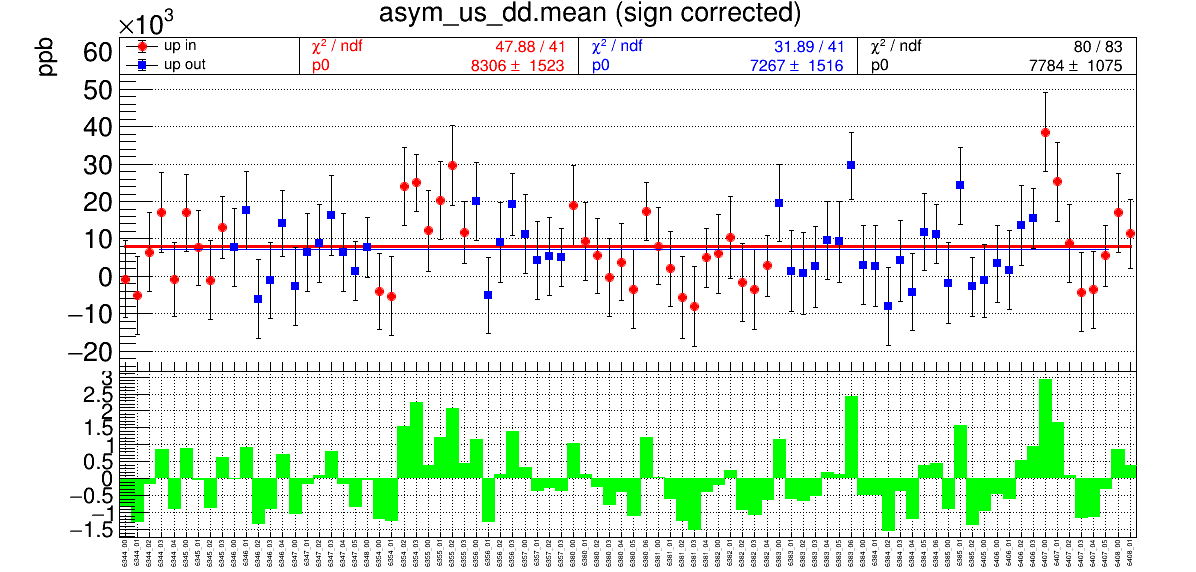
\includegraphics[width=0.9\linewidth]{at/mini_Ca48_asym_us_dd.mean.png}
    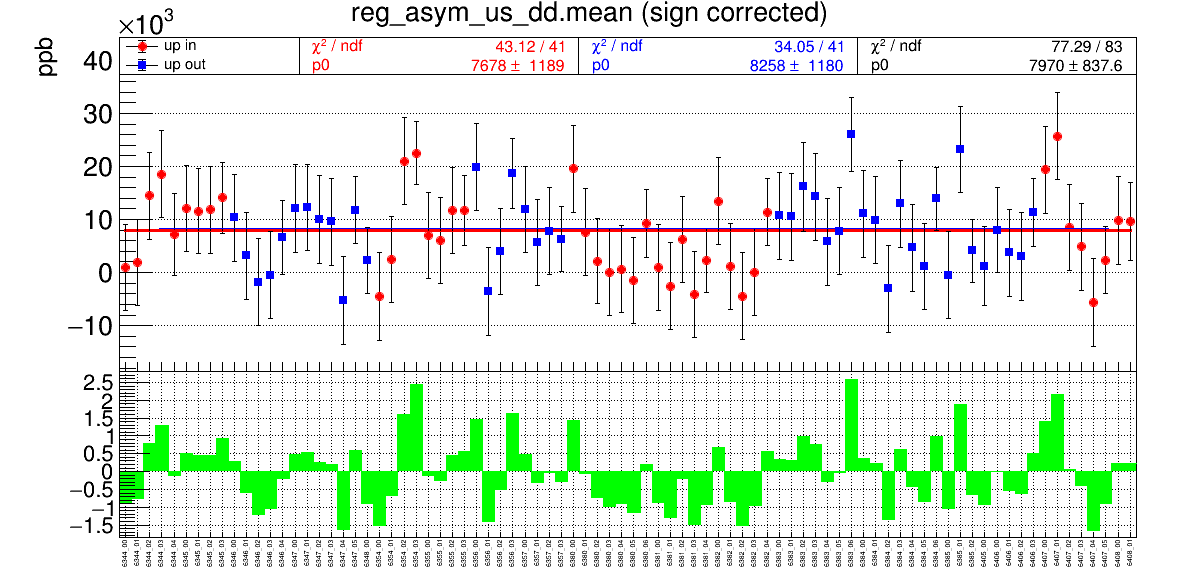
\includegraphics[width=0.9\linewidth]{at/mini_Ca48_reg_asym_us_dd.mean.png}
    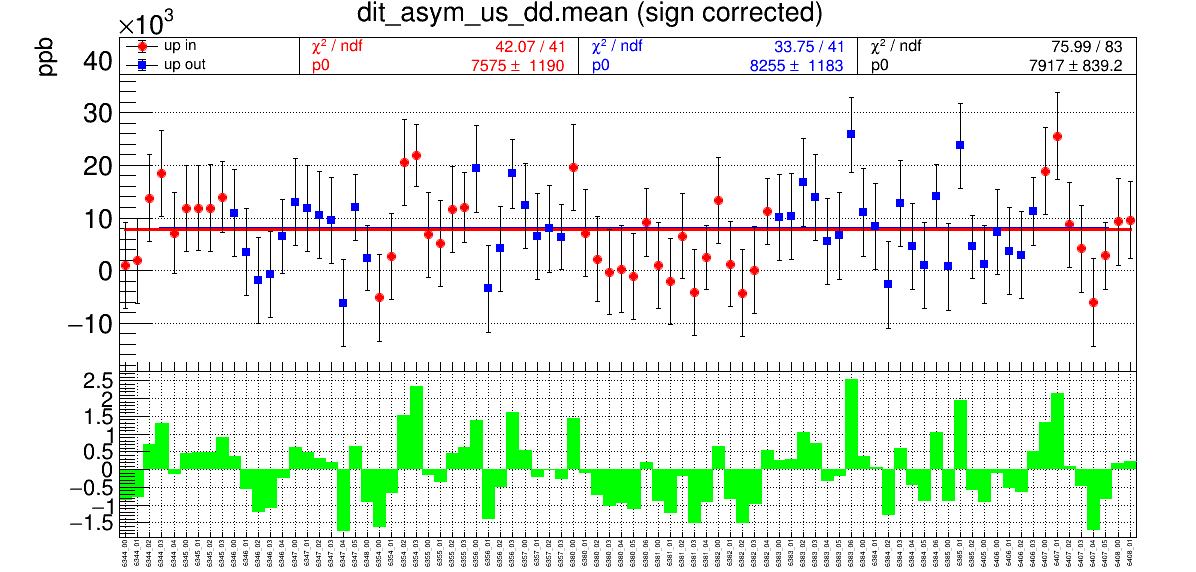
\includegraphics[width=0.9\linewidth]{at/mini_Ca48_dit_asym_us_dd.mean.png}
    \caption{Sign corrected minirun-average of raw, regression corrected and 
    dithering corrected transverse asymmetry of \Ca. Different colors represent
    different IHWP state (in/out). In each plot, the top pad shows the 
    mean and error of the title variable for each minirun, the 3 fit lines indicate
    fitting to IHWP=in, IHWP=out and all datapoints respectively;
    the bottom pad is the pull histogram, which is the ratio of the deviation 
    from the (all datapoints) mean value over each datapoint's error.
    % Regress with the following 5 BPMs: bpm1X, bpm4aY, bpm4eX, bpm4eY, bpm12X.
    % PREX-regression bpms: bpm4aX/Y, bpm4eX/Y, bpmE
    }
    \label{fig:AT_crex_Ca48_miniruns}
\end{figure}

\begin{figure}[H]
    \centering
    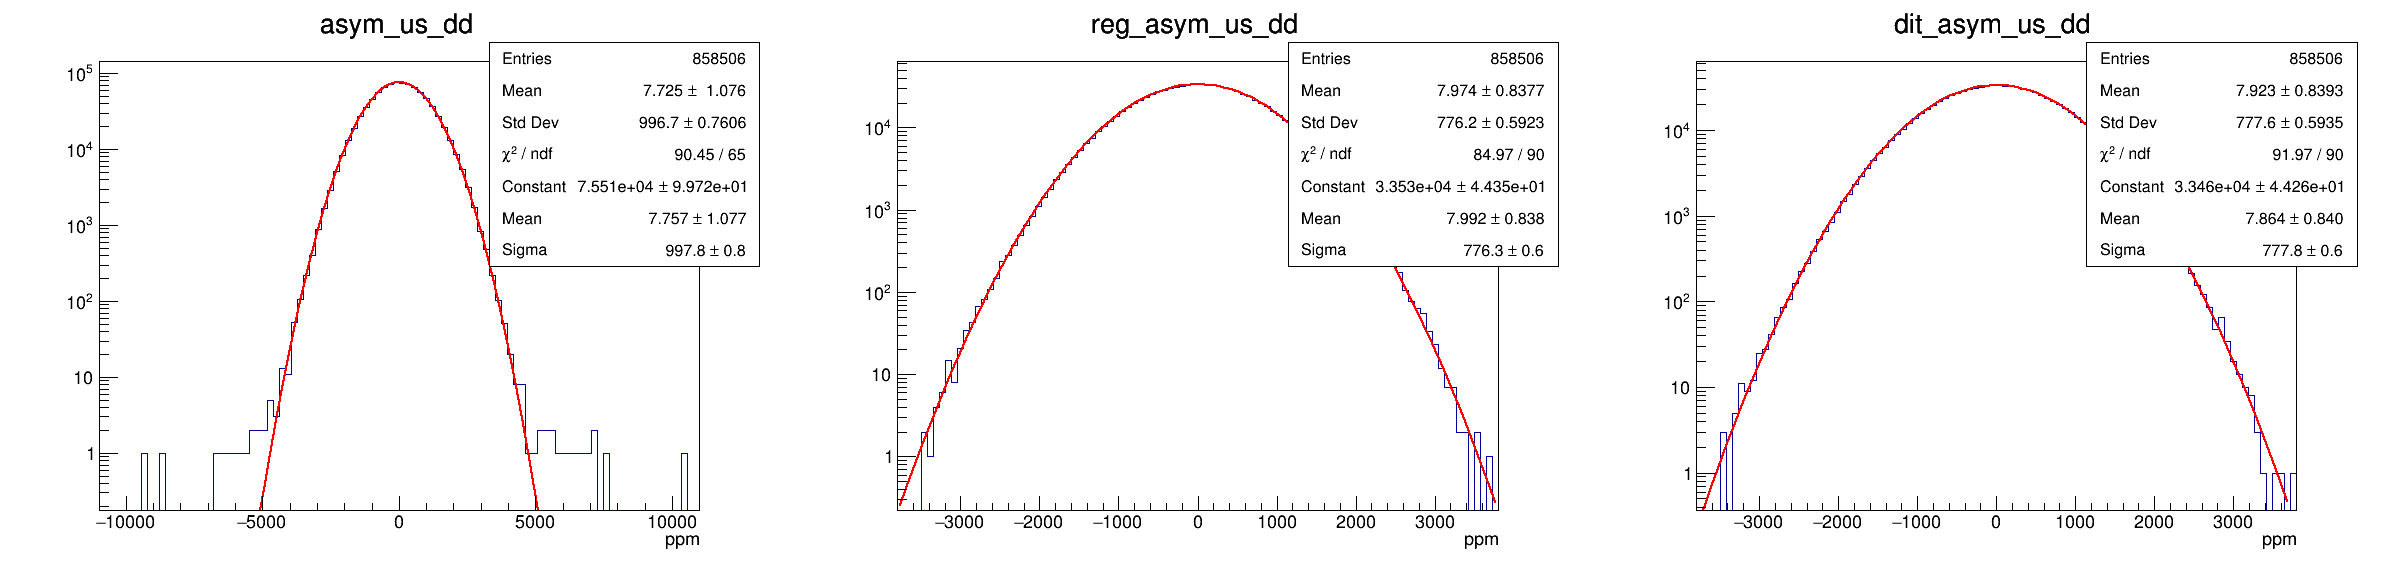
\includegraphics[width=\linewidth]{at/mulplot_Ca48}
    \caption{Mulplot for CREX \Ca. The red line is a Gaussian fit. One can see 
    clearly the how correction reduce the width of the distribution (note that
    the first plot has a larger x-range than the other two).}
    \label{fig:AT_crex_Ca48_mulplot}
\end{figure}

The minirun mean and mulplot mean for each target are summarized in the following
tables.
\begin{table}[!h]
    \scriptsize
    \begin{tabular}{c | r@{ $\pm$ }l r@{ $\pm$ }l r@{ $\pm$ }l | r@{ $\pm$ }l r@{ $\pm$ }l r@{ $\pm$ }l}
	\hline
	\multirow{2}{*}{Target}	& \multicolumn{6}{c|}{Minirun Average (ppb)} & \multicolumn{6}{c}{Mulplot (ppb)}	\\
	\cline{2-13}
	    & \multicolumn{2}{c}{raw}   & \multicolumn{2}{c}{reg}	& \multicolumn{2}{c|}{dit}   & \multicolumn{2}{c}{raw}	& \multicolumn{2}{c}{reg}   & \multicolumn{2}{c}{dit}	\\
	\hline
	\multicolumn{13}{c}{IHWP IN}   \\
	\hline
	\C	& 4205.3	& 1113.7    & 5173.9	& 501.5	    & 5169.4	& 502.1	    & 4129.8  & 1117.7    & 5105.0  & 504.9     & 5103.5  & 505.6   \\ 
	\ca	& 3055.9	& 1762.7    & 5507.5	& 419.3     & 5517.4	& 420.7	    & 2979.8  & 1763.3    & 5501.8  & 420.0     & 5511.7  & 421.4   \\   
	\Pb	& -266.2	& 974.2     & 54.9  	& 183.5     & 27.7  	& 185.7	    & -386.2  & 958.3     & 101.5   & 180.3     & 70.2    & 182.5   \\   
	\hline
	\multicolumn{13}{c}{IHWP OUT}   \\
	\hline
	\C	& 6111.0	& 992.1	    & 5685.5	& 437.4	    & 5740.6	& 437.9	    & 6055.9  & 995.8     & 5619.1  & 440.1     & 5669.4  & 440.6   \\ 
	\ca	& 5707.4	& 1687.6    & -679.8	& 443.0     & 5093.7	& 399.6	    & 5775.6  & 1687.8    & 5033.6  & 396.7     & 5033.6  & 399.2   \\   
	\Pb	& -132.7	& 927.4     & -52.3 	& 176.1     & -26.1 	& 178.7	    & -86.5   & 922.7     & -73.2   & 174.9     & -86.2   & 209.0   \\   
	\hline
	\multicolumn{13}{c}{COMBINED}   \\
	\hline
	\C	& 5267.8	& 740.8	    & 5464.5	& 329.6	    & 5493.9	& 330.0	    & 5209.7  & 743.5     & 5393.2  & 331.8     & 5427.0  & 332.2   \\ 
	\ca	& 4439.2	& 1219.0    & 5276.3	& 288.3     & 5294.7	& 289.7	    & 4444.9  & 1219.7    & 5275.3  & 288.5     & 5293.9  & 290.0   \\   
	\Pb	& -196.2	& 671.7     & -0.9  	& 127.0     & -0.3  	& 128.8	    & -231.5  & 664.7     & 11.3    & 125.5     & 70.2    & 182.5   \\   
	\hline
    \end{tabular}
    \caption{PREX-II raw and beam corrected transverse asymmetry}
\end{table}

\begin{table}[!h]
    \scriptsize
    \begin{tabular}{c | r@{ $\pm$ }l r@{ $\pm$ }l r@{ $\pm$ }l | r@{ $\pm$ }l r@{ $\pm$ }l r@{ $\pm$ }l}
	\hline
	\multirow{2}{*}{Target}	& \multicolumn{6}{c|}{Minirun Average (ppb)} & \multicolumn{6}{c}{Mulplot (ppb)}	\\
	\cline{2-13}
	    & \multicolumn{2}{c}{raw}   & \multicolumn{2}{c}{reg}	& \multicolumn{2}{c|}{dit}   & \multicolumn{2}{c}{raw}	& \multicolumn{2}{c}{reg}   & \multicolumn{2}{c}{dit}	\\
	\hline
	\multicolumn{13}{c}{IHWP IN}   \\
	\hline
	\C	& 6815.5    & 1397.2	& 7767.7    & 1182.2	& 7660.5    & 1183.4	& 6885.1    & 1397.9	& 7725.7    & 1182.1	& 7618.8 & 1183.3	\\ 
	\ca     & 8661.9    & 1643.5	& 8777.5    & 1265.2	& 8764.4    & 1267.5	& 8581.7    & 1645.3	& 8743.9    & 1265.3	& 8733.3 & 1267.6	\\ 
	\Ca     & 8306.5    & 1523.3   	& 7677.5    & 1188.9	& 7575.2    & 1190.3	& 8275.7    & 1524.9	& 7658.9    & 1189.0	& 7553.5 & 1190.3	\\ 
	\Pb	& 2742.6    & 2469.1   	& 3052.4    & 2285.9	& 3079.7    & 2288.1	& 2771.1    & 2469.6	& 3101.8    & 2286.2	& 3129.9 & 2288.3	\\ 
	\hline
	\multicolumn{13}{c}{IHWP OUT}   \\
	\hline
	\C	& 8607.9	& 1558.2    & 8789.1	& 1313.5    & 8791.5	& 1314.6    & 8512.9    & 1558.8	& 8778.2    & 1313.6	& 8780.0    & 1314.7	\\      
	\ca      & 8023.6	& 1751.5    & 7967.4	& 1353.3    & 7994.2	& 1355.0    & 8168.4    & 1755.1	& 7960.2    & 1353.4	& 7987.0    & 1355.2	\\      
	\Ca      & 7267.1	& 1516.3    & 8257.8	& 1180.2    & 8254.7	& 1183.3    & 7184.5    & 1517.6	& 8267.8    & 1180.3	& 8270.3    & 1183.5	\\      
	\Pb	& 2089.1	& 2456.4    & 2420.2	& 2263.4    & 2456.9	& 2266.2    & 2075.1    & 2456.8	& 2401.2    & 2263.8	& 2440.7    & 2266.6	\\      
	\hline
	\multicolumn{13}{c}{COMBINED}   \\
	\hline
	\C	& 7614.4	& 1040.3    & 8224.8	& 878.7     & 8166.8	& 879.5	    & 7600.8    & 1040.8	& 8235.1    & 878.8 	& 8177.3    & 879.6	\\      
	\Ca      & 8363.1	& 1198.5    & 8399.7	& 924.2     & 8405.0	& 925.6	    & 8377.3    & 1200.4	& 8383.5    & 924.3 	& 8390.4    & 925.7 	\\        
	\Ca  	& 7784.4	& 1074.7    & 7969.8	& 837.6     & 7916.9	& 839.2	    & 7725.4    & 1075.7	& 7974.4    & 837.7 	& 7923.5    & 839.3 	\\        
	\Pb      & 2414.2	& 1741.4    & 2733.1	& 1608.4    & 2765.3	& 1610.1    & 2422.6    & 1741.7	& 2751.0    & 1608.6	& 2784.8    & 1610.4	\\        
	\hline
    \end{tabular}
    \caption{PREX-II raw and beam corrected transverse asymmetry}
\end{table}

\begin{comment}
    & 343.4 & 154.8 & 155.1
    & 379.9 & 91.0  & 91.4
    & 493.9 & 93.0  & 94.1
    & 345.4 & 152.9 & 153.0
    & 387.2 & 91.3  & 91.9
    & 495.3 & 93.5  & 95.3
    & 344.5 & 153.7 & 153.9
    & 383.6 & 91.2  & 91.7
    & 494.5 & 93.2  & 94.6


\begin{table}
    \scriptsize
    \begin{tabular}{c | c c c | c c c}
	\hline
	\multirow{2}{*}{Target}	& \multicolumn{3}{c|}{Minirun Average (ppm)} & \multicolumn{3}{c}{Mulplot (ppm)}	\\
	\cline{2-7}
	    & raw	& reg	& dit	& raw	& reg	& dit	\\
	\hline
	\multicolumn{7}{c}{IHWP IN}   \\
	\hline
	C	& 659.82  & 558.10  & 558.71  & 659.84  & 557.97  & 558.56	\\
	Ca40    & 933.96  & 717.96  & 719.28  & 933.69  & 718.04  & 719.32	\\
	Ca48    & 994.35  & 775.30  & 776.19  & 994.78  & 775.61  & 776.50	\\
	Pb	& 1262.78 & 1168.89 & 1170.02 & 1261.95 & 1168.23 & 1169.35	\\
	\hline
	\multicolumn{7}{c}{IHWP OUT}   \\
	\hline
	C	& 8607.92 & 1558.19	& 8789.05 & 1313.51	& 8791.48 & 1314.60	 \\
	Ca40    & 8023.61 & 1751.48	& 7967.37 & 1353.29	& 7994.17 & 1355.00	 \\
	Ca48    & 7267.11 & 1516.31	& 8257.84 & 1180.23	& 8254.72 & 1183.33	 \\
	Pb	& 2089.10 & 2456.43	& 2420.15 & 2263.44	& 2456.87 & 2266.23	 \\
	\hline
	\multicolumn{7}{c}{COMBINED}   \\
	\hline
	C	& 661.92  & 558.72  & 559.27  & 661.73  & 558.75  & 559.29	\\
	Ca40    & 932.99  & 718.38  & 719.52  & 932.93  & 718.36  & 719.47	\\
	Ca48    & 996.46  & 775.93  & 777.46  & 996.67  & 776.15  & 777.63	\\
	Pb	& 1260.29 & 1163.94 & 1165.22 & 1259.54 & 1163.30 & 1164.57	\\
	\hline
    \end{tabular}
    \caption{Mini-wise average and mulplot average values for each target}
\end{table}
\end{comment}
As shown in above tables, the 2 correction methods -- regression and dithering 
match with each other,
We chose the dithering corrected values to extract transverse asymmetry.
A slug-wise plot of the transverse asymmetry are shown in Fig. \ref{fig:AT_slug} 
\begin{figure}[H]
    \centering
    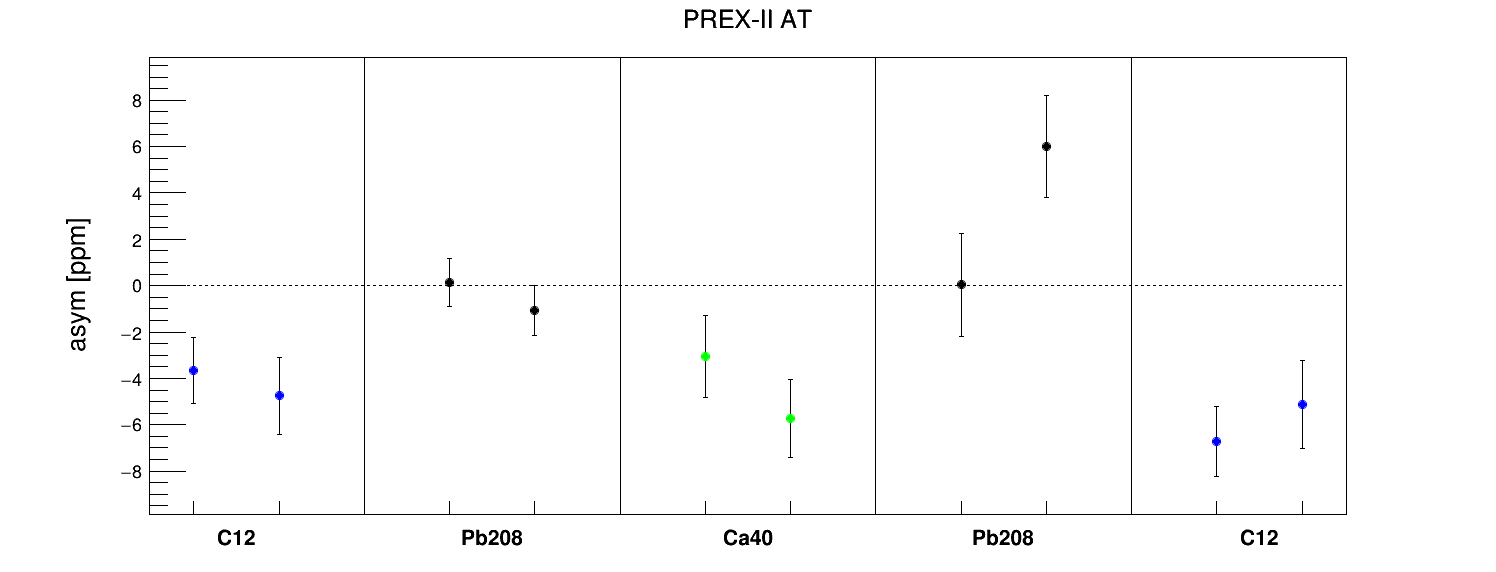
\includegraphics[width=\linewidth]{at/prex_at_slug}
    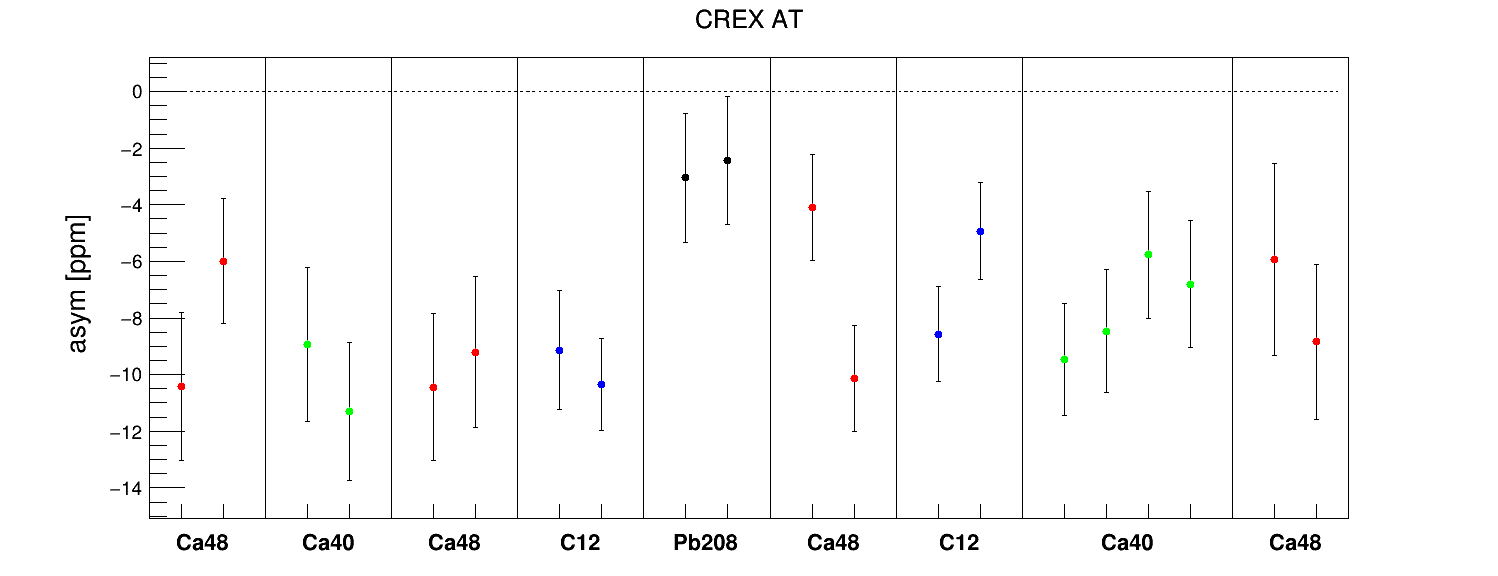
\includegraphics[width=\linewidth]{at/crex_at_slug}
    \caption{Sign corrected transverse asymmetry in chronological order. 
    Each datapoint means one slug.}
    \label{fig:AT_slug}
\end{figure}

%%%%%%%%%%%%%%%%%%%%%%%%%%%%%%%%%%%%%%%%%%%%%%%%
\subsection{Systematic Uncertainties}
Various corrections we made to the raw data will introduce corresponding uncertainties. 
Such as beam false asymmetry, purity correction and detector/monitor non-linearity correction. 
We need to know these correction precisely.

%%%%%%%%%%%%%%%%%%%%%%%%
\subsubsection{Beam Correction}
% https://prex.jlab.org/DocDB/0005/000504/002/Dithering%20and%20Regression.pdf
As said before, we used regression and dithering to extract detector's response
to beam fluctuations, and corrections from these 2 methods agreed with each other.
To count the uncertainty caused by beam correction, we used the difference 
between corrections of these 2 methods. More specifically, 
we found that for most runs, the difference between the corrections
of the most significant BPMs using these 2 methods was less than 5\%, therefore,
a conservative estimation of 5\% of the dithering correction was used as the 
beam correction systematic uncertainty. The dithering slope was target wise, 
the beam correction of each bpm (or their combinations) will be the product of 
the dithering slope and the average difference in each bpm (or their combinations), 
root-sum-square of 5\% of these corrections gave out the uncertainties. 
The result is shown below:

\begin{table}
    \centering
    \begin{tabular}{c c | c c | c c | c c | c}
	\hline
	Exp & Target	
	& \multicolumn{2}{c|}{\thead{$\CA_{raw} \pm d\CA_{raw}$ \\ (ppb)}}    
	& \multicolumn{2}{c|}{\thead{$\CA_{dit}  \pm d\CA_{dit}$ \\  (ppb)}}	
	& \multicolumn{2}{c|}{\thead{$\Delta\CA \pm d(\Delta\CA)$ \\ (ppb)}}	
	& $d\Delta\CA/d\CA_{dit}$\\
	\hline
	\multirow{3}{*}{PREX-II}
	    & \C    & -5268	& 741	& -5494	& 330	& 226.1	& 29.4	& 9\%	\\ 
	    & \ca   & -4439	& 1219	& -5295	& 290	& 195.9 & 42.4	& 15\%	\\ 
	    & \Pb   & 196.2	& 672	& 0.257	& 129	& 855.5 & 71.0	& 55\%	\\ 
	\hline
	\multirow{4}{*}{CREX}
	    & \C    & -7614	& 1040	& -8167	& 880	& 552.4 & 37.8	& 4\%	\\ 
	    & \ca   & -8363	& 1198	& -8405	& 926	& 351.1 & 48.9	& 5.3\%	\\ 
	    & \Ca   & -7784	& 1075	& -7917	& 839	& 41.9  & 86.7	& 10\%	\\ 
	    & \Pb   & -2414	& 1741	& -2765	& 1610	& 132.5 & 27.8	& 2\%	\\ 
	\hline
    \end{tabular}
    \caption{Beam correction to transverse asymmetry.}
\end{table}

%%%%%%%%%%%%%%%%%%%%%%%%
\subsubsection{Purity Correction}
For target purity correction, we need to consider only the \Pb and \Ca target.
As we will discuss in the following chapter, the contamination in the \Pb target
come from the diamond foils sandwiching the \Pb foil to cool the target, while
the impurity in \Ca target is mainly the \ca isotope. The \ca target has an abundance
larger than 99.6\%, so we regard it as a pure target.

\begin{equation}
    \begin{gathered}
	\CA_{mea} = \frac{R_t\CA_t + \sum_i R_i \CA_i}{R_t + \sum_i R_i} = \frac{\CA_t + \sum_i f_i \CA_i}{1 + \sum_i f_i}  \\
	\CA_t = (1 + \sum_i f_i)\CA_{mea} - \sum_i f_i\CA_i
    \end{gathered}
    \label{eq:AT-asymmetry_correction}
\end{equation}
where $R$ and $\CA$ are the scattering rate and asymmetry of each element, the
subscript t and i mean target and various impurity elements in the target, 
$f_i = \frac{R_i}{R_t}$ is the rate fraction. 
We used simulation to calculate the scattering rate for each different
target, asymmetry value was what we measured.

\begin{equation}
    f_C = \frac{R_C}{R_{Pb}} = 
    \begin{cases}
	0.0671 \pm 0.0057   & E = 0.95\ GeV	\\
	0.6089 \pm 0.0609   & E = 2.2\ GeV	\\
    \end{cases}
\end{equation}

The \Ca case was a little complicated, because the \Ca target was a stack of 3 different
pieces with different purities. The upstream 2 pieces were the remnant of the destroyed
old target with a \Ca abundance of 95.99\%, the downstream piece was a new foil
with a \Ca abundance of 90.04\%. Based on the fact that contaminations were isotope
of \Ca: \ca ($\sim10\%$), ${}^{42}Ca$ ($\sim0.1\%$) and ${}^{44}Ca$ ($\sim0.2\%$), whose 
scattering rate and asymmetry are similar to that of \Ca, so we calculated the
non-\Ca fraction in the \Ca target, which gave the rate fraction as: 
$f(\frac{non-{}^{48}Ca}{{}^{48}Ca}) = 9.07 \pm 0.18 \%$.

Using equation \ref{eq:AT-asymmetry_correction}, we get the purity corrected
asymmetries:
\begin{table}
% https://docs.google.com/spreadsheets/d/1ZI68PgAn_zySKozZ__kHBvxlBmaTMKw9jPSl-EIa91k/edit?pli=1#gid=1243115322
% why cell J4 doesn't follow error propagation
% K3-K9: the formula looks weird
    \centering
    \begin{tabular}{c c | c c }
	\hline
	Exp & Target	
	& \multicolumn{2}{c}{$\CA_{cor}  \pm d\CA_{stat}$ (ppb)}	    \\
	\hline
	\multirow{3}{*}{PREX-II}
	    & \C    & -5494	& 330	 \\ 
	    & \Ca   & -5295	& 290	 \\ 
	    & \Pb   & 369	& 137	 \\ 
	\hline
	\multirow{4}{*}{CREX}
	    & \C    & -8167	& 880	 \\ 
	    & \ca   & -8405	& 926	 \\ 
	    & \Ca   & -7873	& 919	 \\ 
	    & \Pb   & 523	& 2646	 \\ 
	\hline
    \end{tabular}
    \caption{Purity corrected transverse asymmetry. The statistical uncertainties
    were calculated following uncertainty propagation equation.}
\end{table}

%%%%%%%%%%%%%%%%%%%%%%%%
\subsubsection{Detector Non-linearity}
For uncertainty caused by detector non-linearity response to the incoming electron flux,
it was bounded to be $<0.5\%$ in bench tests.
\begin{table}[!h]
    \centering
    \begin{tabular}{c c | c c c}
	\hline
	Exp & Target	& $\CA_{raw}$ (ppb) & $d\CA_{sys}$ (ppb)    & $\frac{d\CA_{sys}}{\CA_{raw}}$   \\
	\hline
	\multirow{3}{*}{PREX-II}
	    & \C    & -5268	& 26	& 0.50\%    \\ 
	    & \ca   & -4439	& 22	& 0.50\%    \\ 
	    & \Pb   & 196.2	& 1	& 0.50\%    \\ 
	\hline
	\multirow{4}{*}{CREX}
	    & \C    & -7614	& 38	& 0.50\%    \\ 
	    & \ca   & -8363	& 42	& 0.50\%    \\ 
	    & \Ca   & -7784	& 39	& 0.50\%    \\ 
	    & \Pb   & -2414	& 12	& 0.50\%    \\ 
	\hline
    \end{tabular}
    \caption{Systematic uncertainty due to detector non-linearity}
\end{table}

For uncertainty come from bcm non-linearity, a conservative estimation of 1\% was used,
as shown in Table \ref{tab:AT_bcm_non-linearity}, the charge asymmetry was minirun-wise average 
value.
\begin{table}[!h]
    \centering
    \begin{tabular}{c c | c c c}
	\hline
	Exp & Target	& $\CA_{q}$ (ppb) & $d\CA_{q}$ (ppb)    & $\frac{d\CA_{q}}{\CA_{q}}$   \\
	\hline
	\multirow{3}{*}{PREX-II}
	    & \C    & -52.863   & 0.5   & 1.00\%    \\ 
	    & \ca   & -104.763  & 1.0   & 1.00\%    \\ 
	    & \Pb   & 140.602   & 1.4   & 1.00\%    \\ 
	\hline
	\multirow{4}{*}{CREX}
	    & \C    & 50.09	& 0.5   & 1.00\%    \\ 
	    & \ca   & 47.81	& 0.5   & 1.00\%    \\ 
	    & \Ca   & 27.35	& 0.3   & 1.00\%    \\ 
	    & \Pb   & -1.61	& 0.0   & 1.00\%    \\ 
	\hline
    \end{tabular}
    \caption{Systematic uncertainty due to BCM non-linearity}
    \label{tab:AT_bcm_non-linearity}
\end{table}

%%%%%%%%%%%%%%%%%%%%%%%%%%%%%%%%%%%%%%%%%%%%%%%%
\subsection{Dynamics}

%%%%%%%%%%%%%%%%%%%%%%%%
\subsubsection{$\phi$ Angle}
% http://ace.phys.virginia.edu/HAPPEX/4179
% http://ace.phys.virginia.edu/HAPPEX/4179
We said above that we chosed the angle $\phi$ to be $90^\circ$, but no way to 
achieve exactly that value. The actually value will be a little deviate from
the designed value, as we measured from the data. We draw the $\sin\phi$ distribution
from data, and then took the average, as shown in the following table:
\begin{table}[!htbp]
    \centering
    \begin{tabular}{c c | c c c}
	\hline
	Exp & Target	& LHRS $\sin\phi$   & RHRS $\sin\phi$	& average   \\
	\hline
	\multirow{3}{*}{PREX-II}
	    & \C    & 0.96660   & 0.96700	& 0.9668    \\ 
	    & \ca   & 0.96430   & 0.96440	& 0.9644    \\ 
	    & \Pb   & 0.96625   & 0.96665	& 0.9665    \\ 
	\hline
	\multirow{4}{*}{CREX}
	    & \C    & 0.96950   & 0.96790	& 0.9687    \\ 
	    & \ca   & 0.97090   & 0.96920	& 0.9701    \\ 
	    & \Ca   & 0.97110   & 0.96880	& 0.9700    \\ 
	    & \Pb   & 0.96980   & 0.96830	& 0.9691    \\ 
	\hline
    \end{tabular}
    \caption{Average $\sin\phi$ values for different AT targets.}
\end{table}

%%%%%%%%%%%%%%%%%%%%%%%%
\subsubsection{$Q^2$}
Similar to the extraction of $\phi$ angle, we draw the $Q^2$ distribution for
each target, and then took the mean value. The results are shown in the
following table:
% http://ace.phys.virginia.edu/HAPPEX/4453
% http://ace.phys.virginia.edu/HAPPEX/4468
\begin{table}[!htbp]
    \centering
    \begin{tabular}{c c | r@{ $\pm$ }l | r@{ $\pm$ }l | r@{ $\pm$ }l r@{ $\pm$ }l}
	\hline
	Exp & Target	
	& \multicolumn{2}{c|}{\thead{LHRS $Q^2$ \\ ($GeV^2$)}} 
	& \multicolumn{2}{c|}{\thead{RHRS $Q^2$ \\ ($GeV^2$)}} 
	& \multicolumn{2}{c}{\thead{Average $Q^2$ \\ ($GeV^2$)}} & \multicolumn{2}{c}{\thead{Average $Q$ \\ ($GeV$)}} \\
	\hline
	\multirow{4}{*}{PREX-II}
	& \C	& 0.0068    & 4E-6  & 0.0066    & 5E-6	& 0.00671   & 3.21E-6	& 0.082	& 1.96E-5	\\
	& \ca  	& 0.0068    & 5E-6  & 0.0067    & 6E-6  & 0.00673   & 4.17E-6  & 0.082	& 2.54E-5	\\
	& \Pb 8	& 0.0065    & 5E-6  & 0.0063    & 6E-6  & 0.00640   & 4.06E-6  & 0.080	& 2.54E-5	\\
	& \Pb 9	& 0.0065    & 4E-6  & 0.0063    & 5E-6  & 0.00640   & 3.50E-6  & 0.080	& 2.18E-5	\\
	\hline
	\multirow{4}{*}{CREX}
	& \C	& 0.0328    & 2E-5  & 0.0334    & 2E-5	& 0.0331    & 1.31E-5  & 0.182	& 3.61E-5	\\
	& \ca  	& 0.0306    & 2E-5  & 0.0309    & 2E-5	& 0.0308    & 1.22E-5  & 0.175	& 3.48E-5	\\
	& \Ca  	& 0.0304    & 1E-5  & 0.0307    & 2E-5	& 0.0306    & 1.07E-5  & 0.175	& 3.05E-5	\\
	& \Pb	& 0.0319    & 3E-5  & 0.0322    & 3E-5	& 0.0320    & 1.99E-5  & 0.179	& 5.56E-5	\\
	\hline
    \end{tabular}
    \caption{Average $Q^2$ values for different AT targets.}
\end{table}

%%%%%%%%%%%%%%%%%%%%%%%%%%%%%%%%%%%%%%%%%%%%%%%%
\subsection{Final Result}
From Eq. \ref{eq:measured_AT}, we can calculate the transverse asymmetry:
\begin{equation}
    \CA_n = \frac{\CA_{cor}}{P_n \cdot \sin\phi}
\end{equation}

The statistical uncertainty was calculated as:
\begin{equation}
    d\CA_n(stat) = \frac{d\CA_{cor}(stat)}{P_n \cdot \sin\phi}
\end{equation}

The systematic uncertainty was calculated as:
\begin{equation}
    \left( \frac{d\CA_n(sys)}{\CA_n} \right)^2 = 
	\left( \frac{d\CA_{cor}(sys)}{d\CA_{cor}} \right)^2
	+ \left( \frac{dP_n}{P_n}\right)^2 
\end{equation}
where
\begin{equation}
    d\CA^2_{cor}(sys) = d\CA^2(det\ nonlin) + d\CA^2(bcm\ nonlin) + d\CA^2(beam\ correction)
\end{equation}
In case of \Pb and \Ca target, we need to include uncertainties from contaminations.
Various systematic uncertainties are summarized in Table \ref{tab:AT_uncertainties}.
\begin{table}[!h]
    \centering
    \begin{tabular}{c c c c | c c c c}
	\hline
	Exp & \multicolumn{3}{c|}{PREX-II}  & \multicolumn{4}{c}{CREX}	\\
	Target	& \C	& \ca	& \Pb	& \C	& \ca	& \Ca	& \Pb	\\
	\hline
	Beam correction & 0.03  & 0.05  & 0.08  & 0.04  & 0.06  & 0.10  & 0.03	\\
	Polarization    & 0.06  & 0.05  & $<0.01$ & 0.08  & 0.08  & 0.08  & $<0.01$	\\
	Non-linearity   & 0.03  & 0.03  & $<0.01$ & 0.05  & 0.05  & 0.05  & 0.01	\\
	Tgt. impurity   & $<0.01$ & $<0.01$ & 0.04  & $<0.01$ & $<0.01$ & 0.10  & 0.80	\\
	Inelastic	& $<0.01$ & $<0.01$ & $<0.01$ & 0.08  & 0.15  & 0.08  & $<0.01$	\\
	\hline	
	Tot. Syst	& 0.07  & 0.08  & 0.09  & 0.13  & 0.18  & 0.19  & 0.75	\\
	Statistical	& 0.38  & 0.34  & 0.16  & 1.05  & 1.10  & 1.09  & 3.15	\\
	Total		& 0.39  & 0.34  & 0.18  & 1.05  & 1.11  & 1.11  & 3.23	\\
	\hline
    \end{tabular}
    \caption{AT uncertainty contributions in unit of ppm}
    \label{tab:AT_uncertainties}
\end{table}

The final result is shown in Table \ref{tab:AT_final_values}:
\begin{table}[!h]
    \centering
    \begin{tabular}{c c | c c c c}
	\hline
	Exp & Target	& \thead{$\CA_n$ \\ (ppm)}   & \thead{$d\CA_{stat}$ \\ (ppm)}	
	& \thead{$d\CA_{sys}$ \\ (ppm)}	& \thead{$d\CA_{stat+sys}$ \\ (ppm)}	\\
	\hline
	\multirow{3}{*}{PREX-II}
	    & \C    & -6.34	& 0.38	& 0.07	& 0.39	\\ 
	    & \ca   & -6.12	& 0.34	& 0.08	& 0.34	\\ 
	    & \Pb   & 0.43	& 0.16	& 0.09	& 0.18	\\ 
	\hline
	\multirow{4}{*}{CREX}
	    & \C    & -9.71	& 1.05	& 0.10	& 1.05	\\ 
	    & \ca   & -9.98	& 1.10	& 0.11	& 1.11	\\ 
	    & \Ca   & -9.35	& 1.09	& 0.17	& 1.11	\\ 
	    & \Pb   & 0.62	& 3.15	& 0.75	& 3.23	\\ 
	\hline
    \end{tabular}
    \caption{Final result of Transverse asymmetry.}
    \label{tab:AT_final_values}
\end{table}

Compare to theoretical calculation \cite{PhysRevC.103.064316}, we confirm 
the anomaly appeared in PREX-I, that is the \Pb transverse asymmetries
are consistently 0 at various $Q$ values, as shown in Fig. \ref{fig:pcrex_AT}. 
As for other light nuclei, they are not far away from theoretical predictions.
\begin{figure}
    \centering
    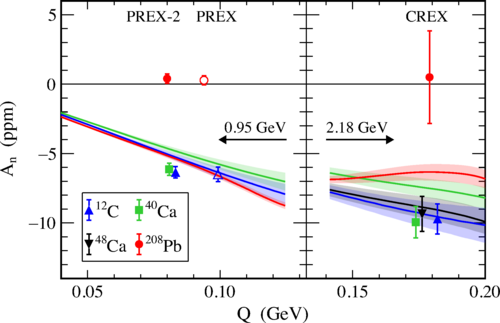
\includegraphics[scale=.5]{at/pcrex_AT}
    \caption{Transverse asymmetry measured in PREX-II/CREX. The PREX-I result
    is also included. Overlapping points are offset slightly in Q to distinguish
    them.}
    \label{fig:pcrex_AT}
\end{figure}

\begin{comment}
    \begin{itemize}
	\item resource: AT plot: https://github.com/cipriangal/prexATplot
	\item regression: which bpm set were used?
	\item dithering: ???
	\item 
    \end{itemize}
\end{comment}

\chapter{Systematic Uncertainties}

Systematic uncertainty control is very important to and a highlight of these 2
high-precision experiments. To achieve a smaller systematic uncertainty, a
combination of fast-control and slow control was employed, which helped 
to cancel many systematic uncertainties brought by the accelerator to the
beam. Except the uncertainty from the machine, another important source
of systematic uncertainties is the detection process, namely the 
acceptance function.

After removing false asymmetry from the beam, we need further correction of the
background asymmetry, namely, target contamination and inelastic scattering,
as shown in Eq.~\ref{eq:background_correction}.
\begin{equation}
    \CA_{pv} = \frac{\CA_{cor}/\CP - \sum_i \CA_i f_i}{1 - \sum_i f_i}
    \label{eq:background_correction}
\end{equation}
Here, $\CA_i$ and $f_i$ refer to the asymmetry and rate fraction of background
processes. In PREX-II, contamination from the diamond foil contributed the
largest background correction.

The uncertainty propagation
\begin{equation}
    (\delta \CA_{pv})^2 = 
      \left( \frac{\partial \CA_{pv}}{\partial \CA_{cor}} \delta \CA_{cor} \right)^2
      + \left( \frac{\partial \CA_{pv}}{\partial \CP} \delta \CP \right)^2
      + \sum_i \left[ \left(\frac{\partial \CA_{pv}}{\partial \CA_i}\delta \CA_i \right)^2 
	 + \left(\frac{\partial \CA_{pv}}{\partial f_i}\delta f_i \right)^2 \right]
\end{equation}

\begin{equation}
    \frac{\partial \CA_{pv}}{\partial \CA_j} = -\frac{f_j}{1 - \sum_i f_i}  \qquad
    \frac{\partial \CA_{pv}}{\partial f_j} = \frac{\CA_{pv} - \CA_j}{1 - \sum_i f_i}
    \label{eq:systematic_uncertainty}
\end{equation}

%%%%%%%%%%%%%%%%%%%%%%%%%%%%%%%%%%%%%%%%%%%%%%%%%%%%%%%%%%%%%%%%%%%%%%%%
\section{$Q^2$ and $\theta$}
Physical interpretation of $\CA_{PV}$ requires precise knowledge
of the scattering angle and corresponding $Q^2$, which were determined using
a watercell target. 
\begin{figure}
    \centering
    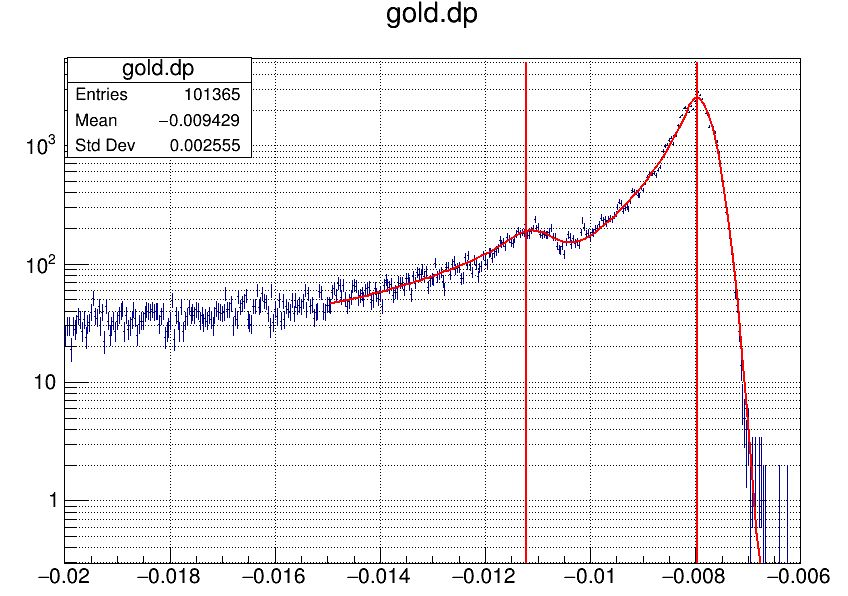
\includegraphics[width=0.5\linewidth]{watercell_Dp}
    \caption{Momentum distribution of the optics run with watercell. The x-axis
    is the relative energy difference: $dp = \frac{p - p0}{p0}$. Plot from Siyu}
    % HRS_optics_siyu
\end{figure}
As we see from Eq.~\ref{eq:scattered_energy}, the energy difference between the
2 elastic peaks is
\begin{equation}
    \Delta E' = E'_O - E'_H = E\left( \frac{1}{1 + \frac{E(1-\cos\theta)}{M_O}} -
    \frac{1}{1 + \frac{E(1-\cos\theta)}{M_H}} \right)
\end{equation}
From above equation, we could calculate the scattering angle from the watercell
target. The advantage of using the watercell target rather than the production
target directly is that the energy difference between the 2 elastic peaks cancels
many uncertainties due to electron detection and trajectory reconstruction, therefore
being more precise.

%%%%%%%%%%%%%%%%%%%%%%%%%%%%%%%%%%%%%%%%%%%%%%%%%%%%%%%%%%%%%%%%%%%%%%%%
\section{Carbon Contamination in PREX-II}
% prex_target_subassy_revB.pdf
The Pb foil is not good thermal conductor, which limited the highest beam current
we could apply. With pure \Pb foil, it will melt at $\sim 10 \mu A$. To help 
dissipate the heat produced by electron bombardment, auxiliary materials -- the 
diamond foils, which are excellent thermal conductor, were used. 
With the help of Diamond foils, the
\Pb target could tolerate up to $\gtrsim 100\ mu A$. Besides, \C is isoscalar, and spin-0 
nucleus, whose PV asymmetry is well-measured (FIXME), so the background is 
well-understood. 

For CREX, Ca48 has good thermal conductivity, so the current can go up to $150\ \mu A$
the contamination mainly come from Ca40 ($\sim 4\%$ FIXME), which is also isoscalar
and spin-0 nucleus, so benign background.

%%%%%%%%%%%%%%%%%%%%%%%%
\subsubsection{Target Thickness}
The \Pb foil was $0.5\ mm$ thick, the upstream and downstream diamond foils 
were half the \Pb thickness, as shown in Table~\ref{tab:target_thickness}.

% https://prex.jlab.org/DocDB/0004/000446/001/target_thickness_errors.txt
The target foils' thicknesses were measured differently. The diamond foil's 
thickness was measured directly using calipers with an accuracy of $0.0005 \ in$ ($0.0127 \ mm$).
Given diamond foil's thickness of $1\ in$ ($0.255 \ mm$), an estimation of 5\% 
relative error was reasonable. Foil to foil variations were small than 5\% (the
largest variation was 3.6\%), as shown in Table~\ref{tab:target_thickness}.

As for the \Pb foil, its thickness (area density) was inferred from its mass 
and area, which was calculated from the measurement of its four corners ($\rho t = \frac{m}{A}$). 
So the final result was average over the whole foil, but the rastered beam 
didn't occupy the whole area, that was a source of uncertainty. The small irregular
in the edge (corner) was another error. A conservative estimation of the systematic
uncertainty of \Pb foil was also 5\%. Again, variations from foil to foil were 
smaller than that (the largest variation being 3.8\%).

\begin{table}[!htbp]
    \centering
    \begin{tabular}{c | c | c c c c}
	\hline
	position    & target& \makecell{Upstream \\ ($mg/cm^2$)}    & \makecell{Center \\ ($mg/cm^2$)}     & \makecell{Downstream \\ ($mg/cm^2$)}   & runs  \\
	\hline
	1   & C-Pb-C	    & 88    & 556   & 88    & \\
	2   & D\#I-Pb-D\#J      & 90    & 557   & 90    & \\
	\hline
	3   & C-208Pb\#1-C    & 88    & 620   & 88    & \\
	4   & Carbon 1\%    &       & 445   &	    & \\
	\hline
	5   & \color{red}{D\#A-208Pb\#2-D\#B}  & 89.0  & 632   & 88.6  & 3134-3636 \\
	6   & D\#C-208Pb\#3-D\#D  & 88.2  & 626   & 90.7  & \\
	7   & D\#E-208Pb\#4-D\#F  & 89.6  & 628   & 91.9  & \\
	8   & \color{red}{D\#G-208Pb\#5-D\#20} & 86.8  & 632   & 90    & 4372-4607 \\
	9   & \color{red}{D\#1-208Pb\#6-D\#2}  & 90    & 618   & 90    & 4865-4980 \\
	10  & \color{red}{D\#3-208Pb\#7-D\#4}  & 90    & 639   & 90    & 4608-4864 \\
	11  & \color{red}{D\#5-208Pb\#8-D\#6}  & 90    & 620   & 90    & 4147-4370 \\
	12  & \color{red}{D\#7-208Pb\#9-D\#8}  & 90    & 615   & 90    & 3822-4146 \\
	13  & \color{red}{D\#9-208Pb\#10-D\#10}& 90    & 623   & 90    & 3644-3821 \\
	\hline
	14  & C-Hole	    &       & N/A   &       & \\
	15  & \color{red}{\Ca}	    &       & 1016  &       & \\
	16  & \ca	    &       & 1004  &       & \\
	\hline
    \end{tabular}
    \caption{Target thickness of each target in the production ladder. 
    Name convention: upstream material\#label - central material\#label - downstream material\#label. 
    Pb208 foils count from 1 to 10, diamond foils count 1-10, A-G, I, J, 20. 
    The first 2 Pb targets are natural Pb foil, not pure \Pb isotope foil. 
    The 3rd Pb target is sandwiched by graphite, not diamond. Red color marks
    out the targets we used in PREX-II and CREX. To convert the number to real 
    thickness, use the density of $\rho_D = 3.52\ g/cm^3$ and $\rho_{208Pb} 
    = 11.38 \ g/cm^3$.}
    \label{tab:target_thickness}
% in simulation, the density values were 3.515 (diamond) and 11.34 (Pb208) respectively -- from wiki
\end{table}

%%%%%%%%%%%%%%%%%%%%%%%%
\subsubsection{Simulation}
In the simulation, the \Pb foil thickness was set to $0.552\ mm$ ($628.176\ mg/cm^2$), 
upstream diamond foil $0.2554\ mm$ ($89.9008\ mg/cm^2$) and downstream diamond 
foil $0.2556\ mm$ ($89.9712\ mg/cm^2$). The central point angle being $4.74^\circ$,
and raster size $6\ mm \times 4\ mm$. 
Only simple cuts were applied to the simulation, as shown below.

\begin{lstlisting}[float,style=C][H]
    xcol != -333 && xvdc != -333    // collimator and vdc see the track
    && CollimatorL(xcol, ycol)	// Q1 collimator geometry cut
    && (nuclA == 12 || nuclA == 208)
    && Pz_peak- Pz < pcut	// radiative tail cut; cut only on lower side
\end{lstlisting}
where Pz was the post target electron momentum, Pz peak $948.97\ MeV$ 
was the momentum peak without momentum cut. With this cut, we could count the scattering
rate from \C and \Pb directly and calculate the ratio between them.

\begin{figure}[H]
    \centering
    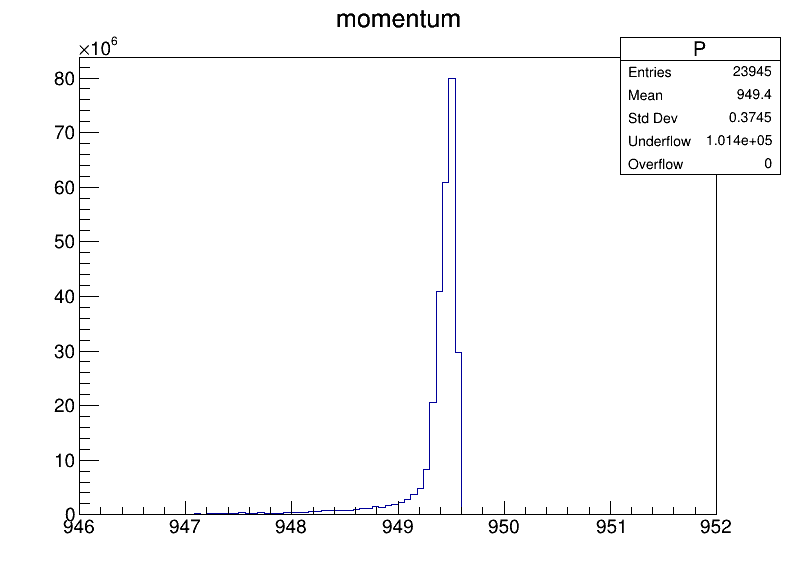
\includegraphics[width=0.5\linewidth]{prex_C_contamination_P}
    \caption{Post target electron momentum distribution. The lower end tail comes 
    from multi-scattering and radiation.}
\end{figure}

The goodness of simulation could be checked by comparison to optics data.
\begin{table}
    \centering
    \begin{tabular}{c c c | c c c c | c c}
	\hline
	\multicolumn{2}{c}{target thickness}	& \multirow{2}{*}{\makecell{p cut \\ (MeV)}}	& \multicolumn{4}{c|}{post target $Q^2$ ($GeV^2$)}   & \multicolumn{2}{c}{Asym ($ppm$)}	\\
	\cline{4-7}
	Pb & C	&   & Pb & C & C (US)	& C (DS) & Pb    & C \\
	\hline
	-5\%	& -5\%	& 2.2	& 0.00625   & 0.00658	& 0.00658   & 0.00658	& 0.55774   & 0.53861 \\
	-5\%	&  0\%	& 2.2	& 0.00626   & 0.00656	& 0.00658   & 0.00654	& 0.55809   & 0.53776 \\
	-5\%	&  5\%	& 2.2	& 0.00627   & 0.00658	& 0.00658   & 0.00657	& 0.55883   & 0.53932 \\
	 0\%	& -5\%	& 2.2	& 0.00627   & 0.00657	& 0.00657   & 0.00657	& 0.55942   & 0.53917 \\
	 0\%	&  0\%	& 2.2	& 0.00626   & 0.00658	& 0.00657   & 0.00660	& 0.55824   & 0.53936 \\
	 0\%	&  5\%	& 2.2	& 0.00627   & 0.00658	& 0.00658   & 0.00658	& 0.55847   & 0.53847 \\
	 5\%	& -5\%	& 2.2	& 0.00625   & 0.00657	& 0.00655   & 0.00658	& 0.55674   & 0.53696 \\
	 5\%	&  0\%	& 2.2	& 0.00627   & 0.00658	& 0.00659   & 0.00657	& 0.55782   & 0.53808 \\
	 5\%	&  5\%	& 2.2	& 0.00629   & 0.00659	& 0.00659   & 0.00659	& 0.55847   & 0.53962 \\
	\hline
	\multicolumn{3}{c|}{average} & 0.00626	& 0.00658   & 0.00658	& 0.00658   & 0.55820   & 0.53859 \\
	\hline
    \end{tabular}
    \caption{Average post target (left arm) $Q^2$ for various thickness configurations. 
    As expected, the $Q^2$ doesn't change with varied foil thicknesses. There is
    some fluctuation in the asymmetry values.}
    % why the C $Q^2$ is a little larger than that of Pb:
    % different scattering angle?
    \label{tab:prex_C_contam_Q2}
\end{table}
From which we can calculate the combined $Q^2$ value
\begin{equation*}
    Q^2 = \frac{R_C Q^2_C + R_{Pb} Q^2_{Pb}}{R_C + R_{Pb}} 
	= \frac{6.71\%\times 0.00658 + 0.00629}{6.71\% + 1} = 0.00629
\end{equation*}

\begin{comment}
\begin{landscape}
    \begin{table}
    \centering
    \begin{tabular}{c c c | c c c c c c c c c c}
	\hline
	\multicolumn{2}{c}{target thicknesses}	& \multirow{2}{*}{\makecell{p cut \\ (MeV)}}	& \multicolumn{2}{c}{$Q^2$ Pb ($GeV^2$)}    & \multicolumn{2}{c}{$Q^2$ C}	& \multicolumn{2}{c}{$Q^2$ C US}  & \multicolumn{2}{c}{$Q^2$ C DS}  & \multicolumn{2}{c}{Asym ($ppm$)}	\\
	Pb & C	&   & vertex	& post vertex	& V	& P-V	& V & P-V   &V	& P-V	& Pb	& C \\
	\hline
	-5\%	& -5\%	& 2.2	& 0.00608   & 0.00625   & 0.00649   & 0.00658	& 0.00641   & 0.00658	& 0.00658   & 0.00658	& 0.55774   & 0.53861 \\
	-5\%	&  0\%	& 2.2	& 0.00609   & 0.00626   & 0.00648   & 0.00656	& 0.00643   & 0.00658	& 0.00654   & 0.00654	& 0.55809   & 0.53776 \\
	-5\%	&  5\%	& 2.2	& 0.00610   & 0.00627   & 0.00650   & 0.00658	& 0.00643   & 0.00658	& 0.00657   & 0.00657	& 0.55883   & 0.53932 \\
	 0\%	& -5\%	& 2.2	& 0.00611   & 0.00627   & 0.00650   & 0.00657	& 0.00643   & 0.00657	& 0.00657   & 0.00657	& 0.55942   & 0.53917 \\
	 0\%	&  0\%	& 2.2	& 0.00609   & 0.00626   & 0.00650   & 0.00658	& 0.00641   & 0.00657	& 0.00660   & 0.00660	& 0.55824   & 0.53936 \\
	 0\%	&  5\%	& 2.2	& 0.00610   & 0.00627   & 0.00649   & 0.00658	& 0.00641   & 0.00658	& 0.00658   & 0.00658	& 0.55847   & 0.53847 \\
	 5\%	& -5\%	& 2.2	& 0.00607   & 0.00625   & 0.00647   & 0.00657	& 0.00637   & 0.00655	& 0.00658   & 0.00658	& 0.55674   & 0.53696 \\
	 5\%	&  0\%	& 2.2	& 0.00609   & 0.00627   & 0.00649   & 0.00658	& 0.00641   & 0.00659	& 0.00657   & 0.00657	& 0.55782   & 0.53808 \\
	 5\%	&  5\%	& 2.2	& 0.00610   & 0.00629   & 0.00650   & 0.00659	& 0.00643   & 0.00659	& 0.00659   & 0.00659	& 0.55847   & 0.53962 \\
	\hline
	\multicolumn{3}{c}{average} &0.00609 & 0.00626	& 0.00649   & 0.00658	& 0.00642   & 0.00658	& 0.00658   & 0.00658	& 0.55820   & 0.53859 \\
    \end{tabular}
	\caption{Average $Q^2$}
    \end{table}
\end{landscape}

I am doubting if I was comparing the same thing. 
In data, $Q^2$ was calculated as:
$$ Q^2 = 2*beamE*P*(1-\cos(\theta))$$
where beamE was the average beam energy (before hitting the target), 
and P was the reconstructed beam energy, or post-target energy 
and $\theta$ was the reconstructed scattering angle 

But in simulation, $Q^2$ was calculated as:
$$ Q^2 = 2*E*Ef*(1-\cos(\theta)) $$
where E was the post vertex beam energy: I made a mistake here, E should be 
pre-vertex beam energy.
$$ Ef = M*E/(M + E*(1-cos(th))) $$
was the theorectical beam energy after elastic scattering and $\theta$ was 
the scattering angle.

Obviously, data and simulation had different definitions:
$$ beamE > E	\quad P < E	\quad P \stacker{?}{\sim} $$
The only good news was that beamE, E, P, Ef were all close to each other. Overall,
the simulation would make the simulation $Q^2$ smaller than that of data. Not
sure how large the uncertainty was.

The only difference here for vertex and post-vertex was the scattering angle,
one was the vertex angle and the other being the post-target scattering angle.

The CREX analysis was comparing the same thing.
\end{comment}

Compare the simulation $Q^2$ to optics data. We saw quite good agreement in left
arm. For the right arm, the larger scattering angle caused a little difference
in $Q^2$ (2\%).
\begin{table}
    \centering
    \begin{tabular}{c | c c}
	\hline
	arm & $\theta$	& $Q^2$ ($GeV^2$)   \\
	\hline
	Left	& $4.748 \pm 0.006$ & $0.00627 \pm 0.00002$	\\
	Right	& $4.813 \pm 0.004$ & $0.00642 \pm 0.00001$	\\
	\hline
    \end{tabular}
    \caption{Average $\theta$ and $Q^2$ for left and right arms. These values were
    combination of Pb and C.}
    \label{tab:prex_C_contam_Q2}
\end{table}

To study the systematic uncertainties, we varied the thickness of \Pb foil and 
diamond foil (total thickness) by 5 percent based on the nominal values, and applied
different momentum cut (varied from 1.8 to 2.6 $MeV$), the result is shown in
Table~\ref{tab:prex_C_contam_rate_thickness} and \ref{tab:prex_C_contam_rate_pcut}. 
$f_c$ is the rate fraction.
\begin{table}[h!]
    \centering
    \begin{tabular}{=c +c | c | +c +c +c +c}
	\hline
	\makecell{\Pb thickness \\ variation}	& \makecell{C thickness	\\ variation}	
	& \makecell{p cut \\ (MeV)} & \makecell{C rate \\ (MHz)}    & \makecell{\Pb rate \\ (MHz)}  
	& $\frac{R_C}{R_{Pb}} (\%)$	& $f_c = \frac{R_C}{R_C + R_{Pb}}$ (\%)	\\
	\hline
	-5\% & -5\% &	  & 1.26E+2 & 1.88E+3 & 6.72 & 6.30	\\
	-5\% &  0\% &     & 1.34E+2 & 1.90E+3 & 7.05 & 6.59   \\
	-5\% &  5\% &     & 1.38E+2 & 1.90E+3 & 7.23 & 6.75   \\
	 0\% & -5\% &     & 1.22E+2 & 1.90E+3 & 6.43 & 6.04   \\
	 \rowstyle{\color{red}}   
	 0\% &  0\% & 2.2 & 1.29E+2 & 1.93E+3 & 6.71 & 6.29   \\
	 0\% &  5\% &     & 1.35E+2 & 1.89E+3 & 7.11 & 6.64   \\
	 5\% & -5\% &     & 1.16E+2 & 1.95E+3 & 5.94 & 5.61   \\
	 5\% &  0\% &     & 1.22E+2 & 1.94E+3 & 6.31 & 5.93   \\
	 5\% &  5\% &     & 1.28E+2 & 1.91E+3 & 6.72 & 6.30   \\
	\hline
    \end{tabular}
    \caption{Scattering rate of the \Pb and diamond foils with different foil
    thicknesses.}
    \label{tab:prex_C_contam_rate_thickness}
\end{table}

\begin{table}[h!]
    \centering
    \begin{tabular}{=c c | +c | +c +c +c +c}
	\hline
	\makecell{\Pb thickness \\ variation}	& \makecell{C thickness	\\ variation}	
	& \makecell{p cut \\ (MeV)} & \makecell{C rate \\ (MHz)}    & \makecell{\Pb rate \\ (MHz)}  
	& $\frac{R_C}{R_{Pb}} (\%)$	& $f_c$ (\%)	\\
	\hline
	\multirow{12}{*}{0\%}	& \multirow{12}{*}{0\%}	&
	    1.80 & 1.24E+2 & 1.86E+3 & 6.68 & 6.26  \\
	& & 1.90 & 1.25E+2 & 1.87E+3 & 6.69 & 6.27  \\
	& & 2.00 & 1.27E+2 & 1.89E+3 & 6.70 & 6.28  \\
	& & 2.05 & 1.27E+2 & 1.90E+3 & 6.70 & 6.28  \\
	& & 2.10 & 1.28E+2 & 1.91E+3 & 6.71 & 6.28  \\
	& & 2.15 & 1.29E+2 & 1.92E+3 & 6.71 & 6.29  \\
	\rowstyle{\color{red}}   
	& & 2.20 & 1.29E+2 & 1.93E+3 & 6.71 & 6.29  \\
	& & 2.25 & 1.30E+2 & 1.94E+3 & 6.72 & 6.30  \\
	& & 2.30 & 1.31E+2 & 1.95E+3 & 6.73 & 6.30  \\
	& & 2.35 & 1.31E+2 & 1.95E+3 & 6.73 & 6.31  \\
	& & 2.40 & 1.32E+2 & 1.96E+3 & 6.74 & 6.32  \\
	& & 2.60 & 1.34E+2 & 1.99E+3 & 6.74 & 6.32  \\
	\hline
    \end{tabular}
    \caption{Scattering rate of the \Pb and diamond foils with different momentum 
    cut.}
    \label{tab:prex_C_contam_rate_pcut}
\end{table}

The uncertainty for each variation was taken to be the absolute difference 
from the nominal value, as shown below:
\begin{table}
    \centering
    \begin{tabular}{c | c c | c c}
	\hline
	variation   & maximum	& diff in $f_C$  & minimum    & diff in $f_C$ \\
	\hline
	Pb & (-5, 0) - (0, 0)	& 2.98E-3   & (+5, 0) - (0, 0)	& -3.55E-3  \\
	C  & (0, +5) - (0, 0)	& 3.53E-3   & (0, -5) - (0, 0)	& -2.49E-3  \\
	p cut	& (2.6) - (2.2)	& 2.93E-4   & (1.8) - (2.2)	& -2.88E-4  \\
	\hline
	total	&   & 4.63E-3	&   & 4.35E-3	\\
	\hline
    \end{tabular}
    \caption{The maximum and minimum difference for each variation. (n1, n2) 
    represents the configuration of target foils' thicknesses. n1 for Pb foil
    and n2 for C foil. (pcut) indicates the p cut value}
    \label{tab:prex_C_contam_error}
\end{table}
Based on Table~\ref{tab:prex_C_contam_error}, a conservative error value 
(the larger one) was used , which gave out the final value of $f_C$
\begin{equation*}
    f_C = 0.0629 \pm 0.005
\end{equation*}

%%%%%%%%%%%%%%%%%%%%%%%%
\subsubsection{Cross Check}
The scattering rate is proportional to the cross section and number of atoms
in unit area. 
\begin{equation}
    R \propto \sigma \times N = \sigma \times \frac{t}{m}
\end{equation}
t and m are, respectively, area density and atomic mass. Therefore
\begin{equation}
    \frac{R_C}{R_{Pb}} = \frac{\sigma_C}{\sigma_{Pb}} \times \frac{t_c}{t_{Pb}} \times \frac{m_{Pb}}{m_C}
\end{equation}
Take $E = 0.95\ GeV$ and $\theta = 4.8^\circ$ (based on Table~\ref{tab:prex_C_contam_Q2}), 
our theorist friends predicted the cross section of C and Pb to be
\begin{equation*}
    \sigma_C = 48.001\ mbarn	\qquad \sigma_{Pb} = 3386.100\ mbarn	
\end{equation*}
% this angle is different from what we used in simulation 4.74

The ratio of $t_C/T_{Pb}$ was calculated as
\begin{table}[!h]
    \centering
    \begin{tabular}{c | c c c | c c c}
	\hline
	target	& \makecell{$t_C$ (US + DS) \\ ($mg/cm^2$)} & \makecell{$t_{Pb}$ \\ ($mg/cm^2$)}	
	& $t_C/t_{Pb}$  & \makecell{main detector \\ error n} & \makecell{weight \\ $1/\sqrt{n}$}    & \makecell{weighted \\ $t_C/t_{Pb}$} \\
	\hline
	Pb208\#2    & 177.6	& 632	& 0.281	& 42.743    & 0.1530	& 0.037 \\
	Pb208\#10   & 180	& 623	& 0.289	& 33.3465   & 0.1732	& 0.043	\\
	Pb208\#9    & 180	& 615   & 0.293 & 28.9264   & 0.1859   	& 0.047	\\
	Pb208\#8    & 180	& 620   & 0.290 & 33.5835   & 0.1726   	& 0.043	\\
	Pb208\#5    & 176.8	& 632   & 0.280 & 36.3435   & 0.1659   	& 0.040	\\
	Pb208\#7    & 180	& 639   & 0.282 & 32.7936   & 0.1746   	& 0.042	\\
	Pb208\#6    & 180	& 618   & 0.291 & 47.6238   & 0.1449   	& 0.036	\\
	\hline
		    & 179.2	& 625.6	& 0.286	&	    & 1.1700	& \color{red} 0.287 \\
	\hline                                                
    \end{tabular}
    \caption{Calculation of weighted $t_C/T_{Pb}$, the main detector error was
    the uncertainty of the main detector mean value (reg\_asym\_us\_avg); the 
    weighted ratio was calculated as $\frac{w_j}{\sum_i w_i} \times \left( t_C/t_{Pb} \right)_j$.}
    \label{tab:ratio_of_area_density}
\end{table}

\begin{table}[!h]
    \centering
    \begin{tabular}{c c | c c c | c c}
	\hline
	E ($GeV$)   & $\theta$  & Target    & $\sigma$ ($mbarn$)    & m & $\frac{R_C}{R_{Pb}}$ (\%) & $f_C$ (\%)    \\
	\hline
	\multirow{2}{*}{0.95}	& \multirow{2}{*}{$4.8^\circ$}	& 
	      \C    & 48.001	& 12.011    & \multirow{2}{*}{7.04} & \multirow{2}{*}{6.57} \\
	\cline{3-5}
	&   & \Pb   & 3386.100	& 207.977   &	& \\
	\hline
    \end{tabular}
    \caption{Theoretical calculation of $f_C$. These are updated values. In the 
    initial study, the scattering angle was chosen to be $4.8^\circ$, with corresponding
    $\sigma_C = 48.001\ mbarn$ and $\sigma_{Pb} = 3386.1\ mbarn$, leading to
    $R_C/R_{Pb} = 7.04\%$ and $f_C = 6.57\%$.}
\end{table}
The theoretical value was 4.6\% higher than the simulation result.

\subsubsection{Contribution to $\CA_{pv}$}
As said before, the asymmetry from carbon scattering was well understood, and
we had a table of cross section and asymmetry for electron-carbon elastic scattering
at various energies and scattering angles, which were numerical solved from the Dirac equation
by our theoretical friends. The same for Pb.
The asymmetry for carbon was taken to be $539.36 \ ppb$ as shown in Table~\ref{tab:prex_C_contam_Q2}
with the nominal Pb and nominal C thicknesses. The uncertainty for it was taken
to be a conservative estimation of 4\%.
\begin{figure}
    \centering
    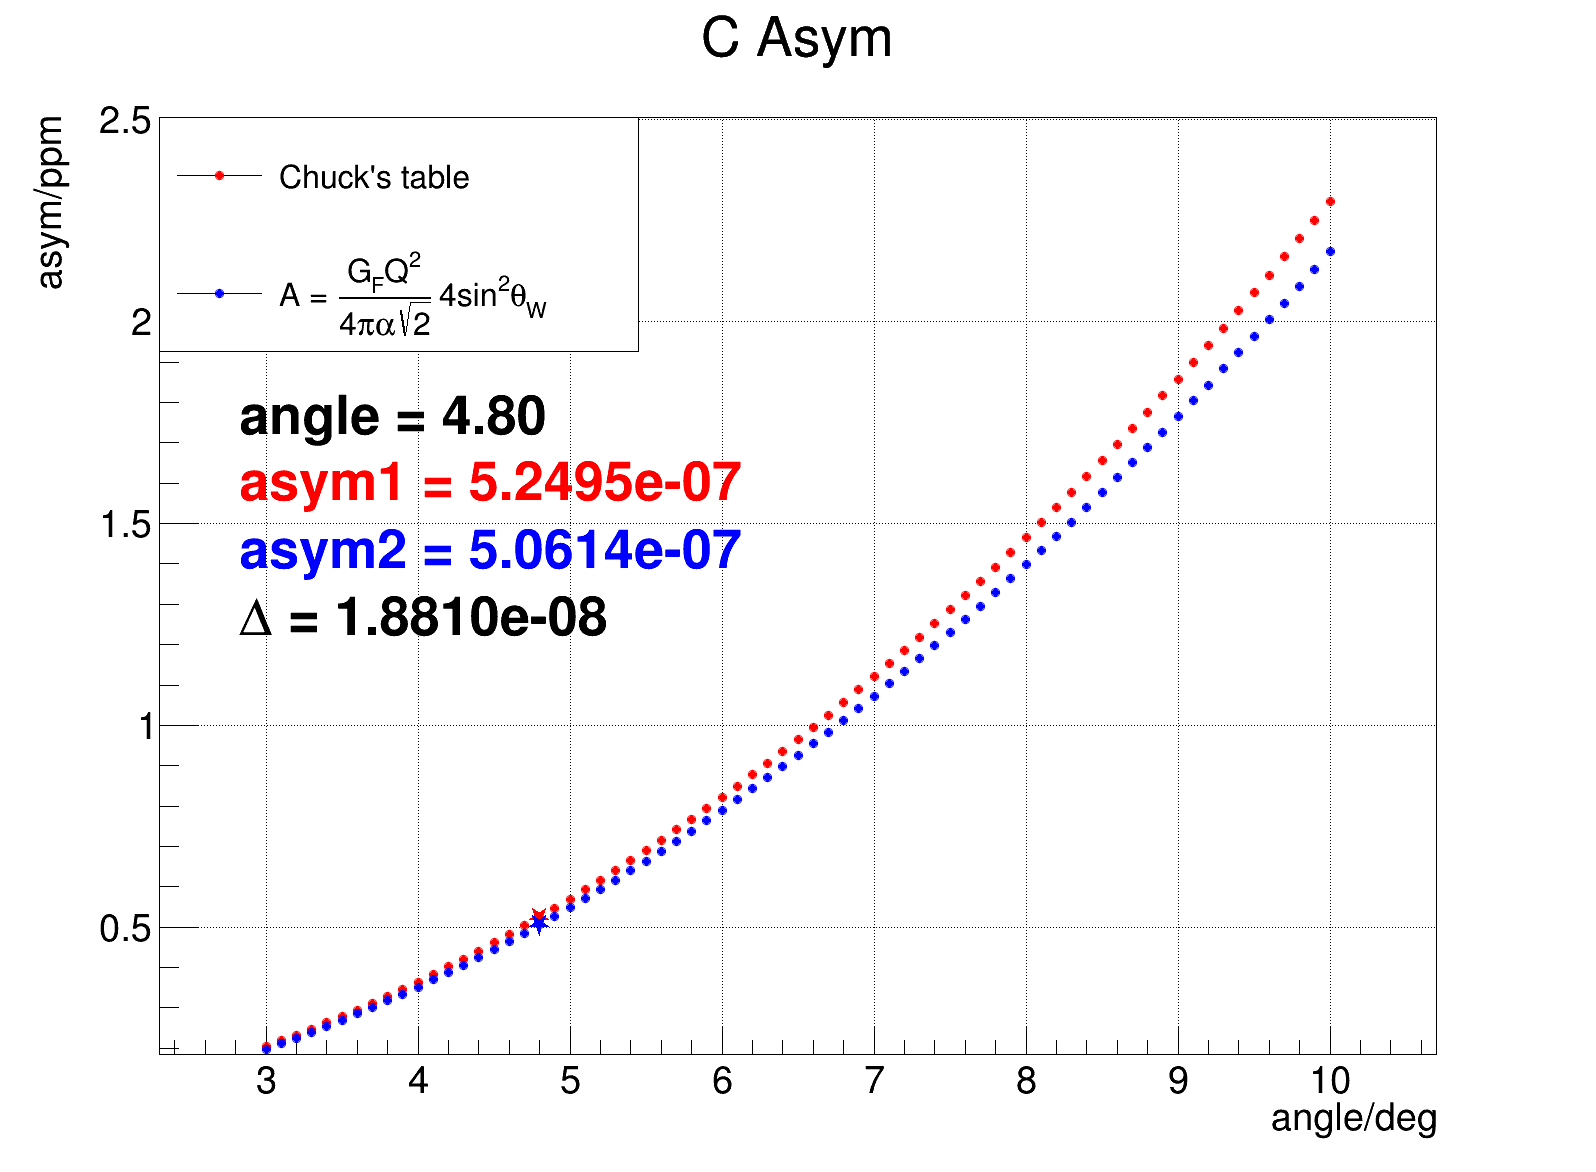
\includegraphics[width=0.49\linewidth]{prex_asym_C}
    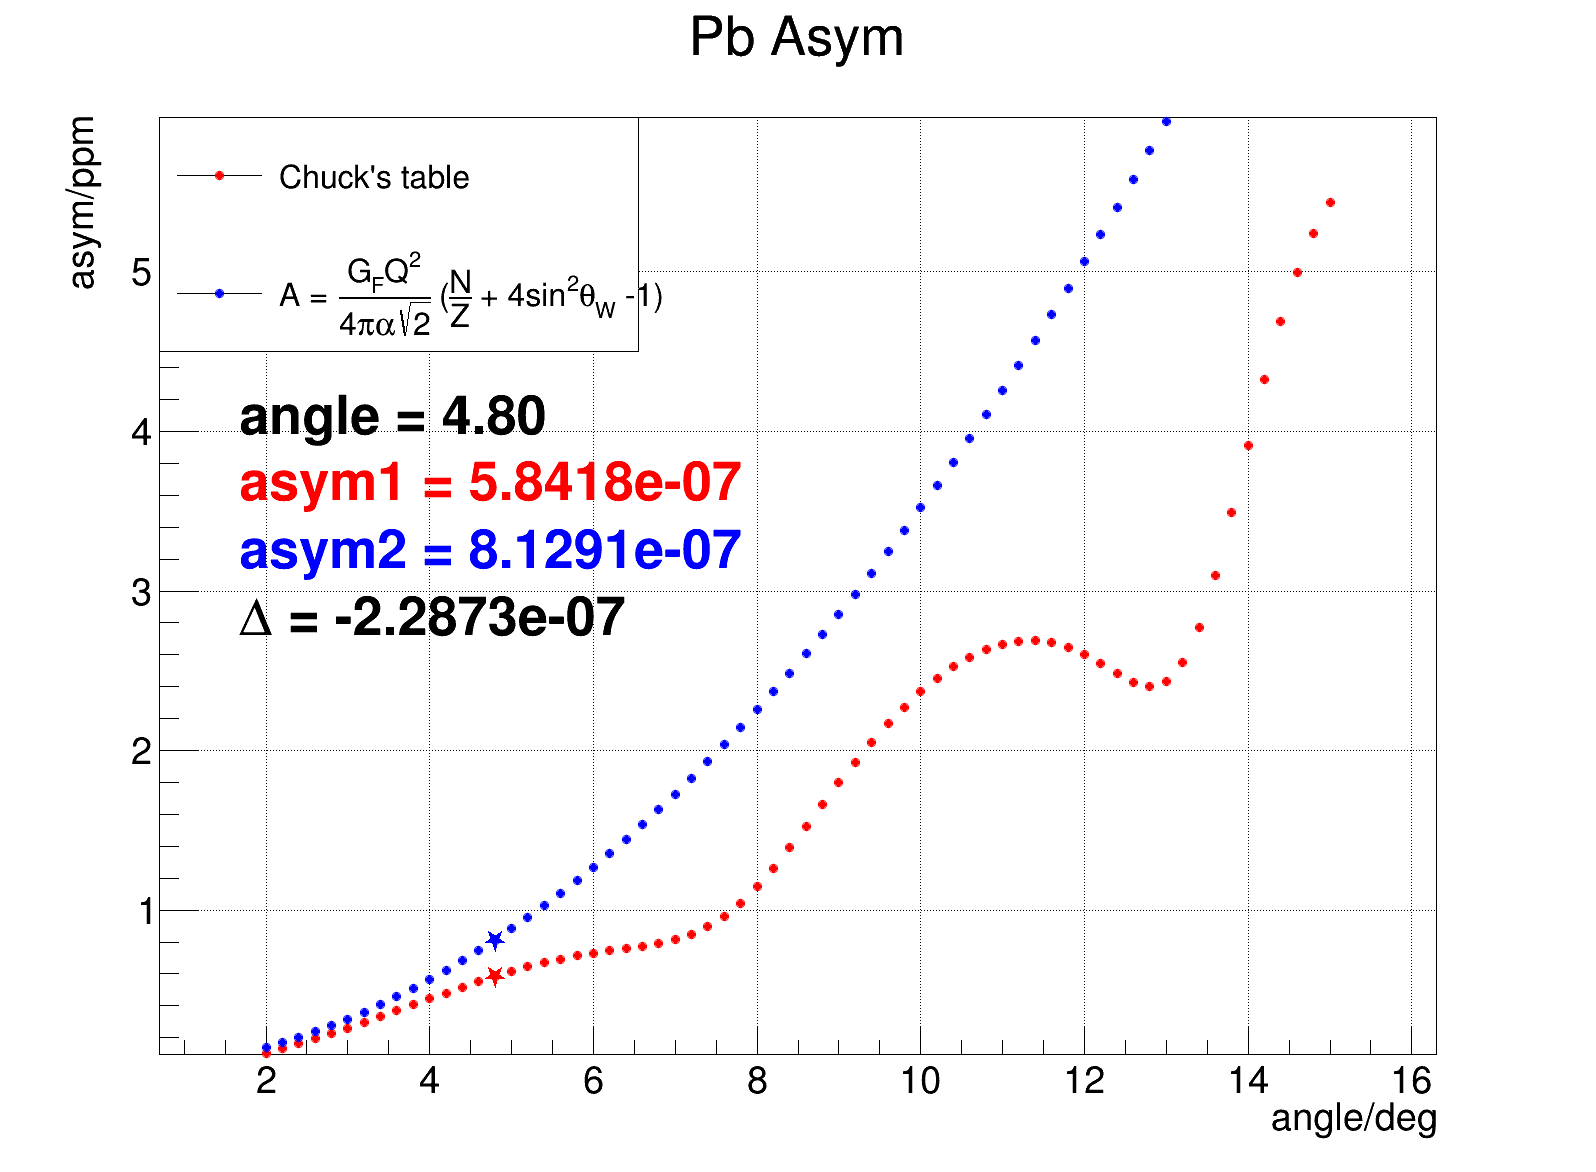
\includegraphics[width=0.49\linewidth]{prex_asym_Pb}
    \caption{Theoretical values of the asymmetry for C and Pb in our experimental 
    dynamics predicted by Chuck's table, which included Coulomb correction, cross
    checked with a Standard Model Born approximation calculation. We see similar
    asymmetry values for C and Pb.}
    \label{prex_asym}
\end{figure}
Using Eq.~\ref{eq:systematic_uncertainty}, we could calculate the uncertainty
contribution to $\CA_{pv}$, summarized in Table~\ref{tab:prex_C_contam}
\begin{equation*}
    \begin{gathered}
	\frac{\partial \CA_{pv}}{\partial \CA_C} \delta \CA_C = 
	-\frac{0.0629}{1 - 0.0629} \times 4\% \times 539.36 = -1.4481\ ppb   \\
	\frac{\partial \CA_{pv}}{\partial f_C}\delta f_C =
	\frac{550 - 539.46}{1 - 0.0629} \times 0.00463 = 0.0521\ ppb	\\
    \end{gathered}
\end{equation*}

\begin{table}
    \centering
    \begin{tabular}{c | c c | c c | c c}
        \hline
	\thead{$\CA_{cor}/\CP$ \\ ($ppb$)}   & \thead{$\CA_C$ \\ ($ppb$)}   & $\frac{\delta\CA_C}{\CA_C}$   & $f_C$ & $\delta f_C$  & \thead{rel. error \\ due to $\CA_C$ } & \thead{rel. error \\ due to $f_C$}\\
        \hline
	549.34	& $539.36$  & 4\%   & 6.29\%	& 0.463\%   & 0.26\%	& 0.01\% \\
        \hline
    \end{tabular}
    \caption{Relative uncertainty due to $\CA_C$ and $f_C$.}
    \label{tab:prex_C_contan}
\end{table}
The uncertainty caused by error in $f_C$ was negligible, and the one from $\CA_C$
was also tiny, which in hindsight, justifies our adoption of the sandwich target.

\begin{comment}
% somehow, the rate derivation was wrong
\bigskip
One could also estimate the rate from measurement. 
\begin{eqaution}
    \sigma = \sqrt{\frac{1}{R/30}}
\end{eqaution}
\begin{table}[!h]
    \centering
    \begin{tabular}{c c c | c c c c c c}
	\hline
	Target	& run	& I $(\mu A)$   & \thead{rms \\ ($ppm$)} & \thead{rms@$70\ \mu A$ \\ ($ppm$)} & \thead{bcm res. \\ ($ppm$)}   & \thead{bpm res. \\ ($ppm$)}   & \thead{cor. rms \\ ($ppm$)}  & \thead{rate \\ ($GHz$)}  \\
	\hline
	C12	& 4133	& 86.2	& 143	& 158.7	& 20	& 25	& 150.4	& 1.326	\\
	D-Pb-D	& 4112	& 67.7	& 93	& 91.5	& 20	& 25	& 82.9	& 4.365	\\
	\hline
    \end{tabular}
    \caption{The corrected rms was calculated as: $\sqrt{\frac{\sigma^2 - \sigma^2_{bcm} - \sigma^2_{bpm}}{1 + 0.26^2}}$}
% why the factor of 0.26
\end{table}
The C graphite target has a thickness of $1.991\ mm$ and a density of 
\end{comment}


%%%%%%%%%%%%%%%%%%%%%%%%%%%%%%%%%%%%%%%%%%%%%%%%%%%%%%%%%%%%%%%%%%%%%%%%
\section{Acceptance Function}
As we said before, the spectrometer acceptance was mainly defined by the Q1 
collimator, but other devices may also have affections on it. And the accepted
area was not tiny ($0.00377 \ sr$), not every point within the acceptance had
the same detection efficiency and cross section asymmetry, therefore what
we measured was actually the average asymmetry over the acceptance:
\begin{equation}
    \CA_{mea} = \frac{\int d\theta \sin\theta A(\theta) \frac{d\sigma}{d\Omega} \epsilon(\theta)}{\int d\theta \sin\theta \frac{d\sigma}{d\Omega} \epsilon(\theta)}
    \label{eq:acceptance_function}
\end{equation}
Here $\epsilon(\theta)$ is the acceptance function, which is defined as
the ratio of electrons that reach the main detector over all scattered
electrons, which depends on the scattering angle $\theta$:
\begin{equation}
    \epsilon(\theta) = \frac{N_{det}(\theta)}{N_{sca}}
    \label{eq:acceptance_definition}
\end{equation}

From Eq.~\ref{eq:acceptance_function}, we see the importance of the acceptance
function. Firstly, it will be a systematic uncertainty of our asymmetry
measurement; and secondly, only with the acceptance function, can we compare
our experimental measurement to theoretical predictions to interpret our
result.

To extract the acceptance function, we had to turn to simulation. Then how
did we know our simulation was correct? We will compare the simulation result
to optics data, and precise match of various kinematic variables between simulation
and data was required. 

When we took optics data, we would put in the sieve slit collimators so that 
we could reconstruct electron trajectory using track info from VDCs 
to match holes in the sieve plane, therefore we could know the scattering angle and 
energy for each electron trajectory.

In terms of simulation, we tuned a few parameters to find out the best
match: so called the best model, which was then used to calculate the acceptance
function. The few parameters we explored were:
\begin{itemize}
    \item Septum current
    \item Q1 collimator shift
    \item Pinch point shift
\end{itemize}

%%%%%%%%%%%%%%%%%%%%%%%%%%%%%%%%%%%%%%%%%%%%%%%%
\subsection{Transportation Matrix}
Due to the existence of various magnetic fields (septum, HRS) from target to detector, 
there is no way to know the exact analytical expression of the transportation
from target to detector, though we can approximate and measure it.

The electron's trajectory can be parameterized as: $\vec{X} = (x, \theta, y, \phi, \delta)^T$ 
w.r.t. to a reference trajectory (usually the central ray). In the transport coordinate, 
$\hat{z}$ is the direction of reference trajectory;
x is the displacement in the dispersive plane relative to the reference 
trajectory, and $\theta$ is electron's `velocity' in the dispersive plane:
$\theta = \frac{\partial x}{\partial z}$; similarly, y and $\phi$ are displacement
and `velocity' in the y-z plane, $\hat{y}$ is oriented such that $\hat{x}$, 
$\hat{y}$, $\hat{z}$ are orthogonal to each other and they form a 
right-handed coordinate $\hat{z} = \hat{x} \times \hat{y}$.
$\delta = \frac{\Delta p}{p}$ represents the fractional deviation of momentum
from that of the reference trajectory. With these definitions, we can expressed
one electron's position along the optical path as a Fourier expansion of the
initial position of $\vec{X}_0$
\begin{equation}
    x_i = \sum_j T_{ij} x_{j,0} + \sum_j \sum_k S_{ijk} x_{j,0}x_{k, 0} + \cdots
\end{equation}
$T_{ij}$ is what we call the transportation matrix, whose elements indicate
the reliance of beam position parameters on each other: $T_{ij} = \frac{\partial x_i}{\partial x_j}$.
First order is a good approximation of the transportation formula. So that we
have:
\begin{equation}
    \begin{pmatrix}
	x   \\
	y   \\
	\theta	\\
	\phi	\\
	\delta	\\
    \end{pmatrix}
    =
    T
    \begin{pmatrix}
	x_{tg}   \\
	y_{tg}   \\
	\theta_{tg}	\\
	\phi_{tg}	\\
	\delta_{tg}	\\
    \end{pmatrix}
    =
    \begin{pmatrix}
	x|x_{tg} & x|y_{tg}   & x|\theta_{tg}	& x|\phi_{tg}    & x|\delta_{tg}    \\
	y|x_{tg} & y|y_{tg}   & y|\theta_{tg}	& y|\phi_{tg}    & y|\delta_{tg}    \\
	\theta|x_{tg} & \theta|y_{tg}   & \theta|\theta_{tg}	& \theta|\phi_{tg}    & \theta|\delta_{tg}    \\
	\phi|x_{tg} & \phi|y_{tg}   & \phi|\theta_{tg}	& \phi|\phi_{tg}    & \phi|\delta_{tg}    \\
	\delta|x_{tg} & \delta|y_{tg}   & \delta|\theta_{tg}	& \delta|\phi_{tg}    & \delta|\delta_{tg}    \\
    \end{pmatrix}
    \begin{pmatrix}
	x_{tg}   \\
	y_{tg}   \\
	\theta_{tg}	\\
	\phi_{tg}	\\
	\delta_{tg}	\\
    \end{pmatrix}
\end{equation}
The `tg' subscript means corresponding values at the target plane. With this matrix, we can
propagate backward (inverse of T) to calculate electron position at the exit 
of the target from what we detect using VDCs. Usually we calculate the beam
position on the focal plane $\vec{X}_{fp}$, then the beam position on the target
plane will be: 
\begin{equation}
    \vec{X}_{tg} = T^{-1} \vec{X}_{fp}
    \label{eq:reconstruction}
\end{equation}
The reason that we don't use BPM to `measure' beam position/angle on target is that 
multi-scattering/radiation inside the target foil will distort the beam trajectory. 

A typical HRS transportation plot looks like Fig. \ref{fig:hrs_transport}:
\begin{figure}[H]
    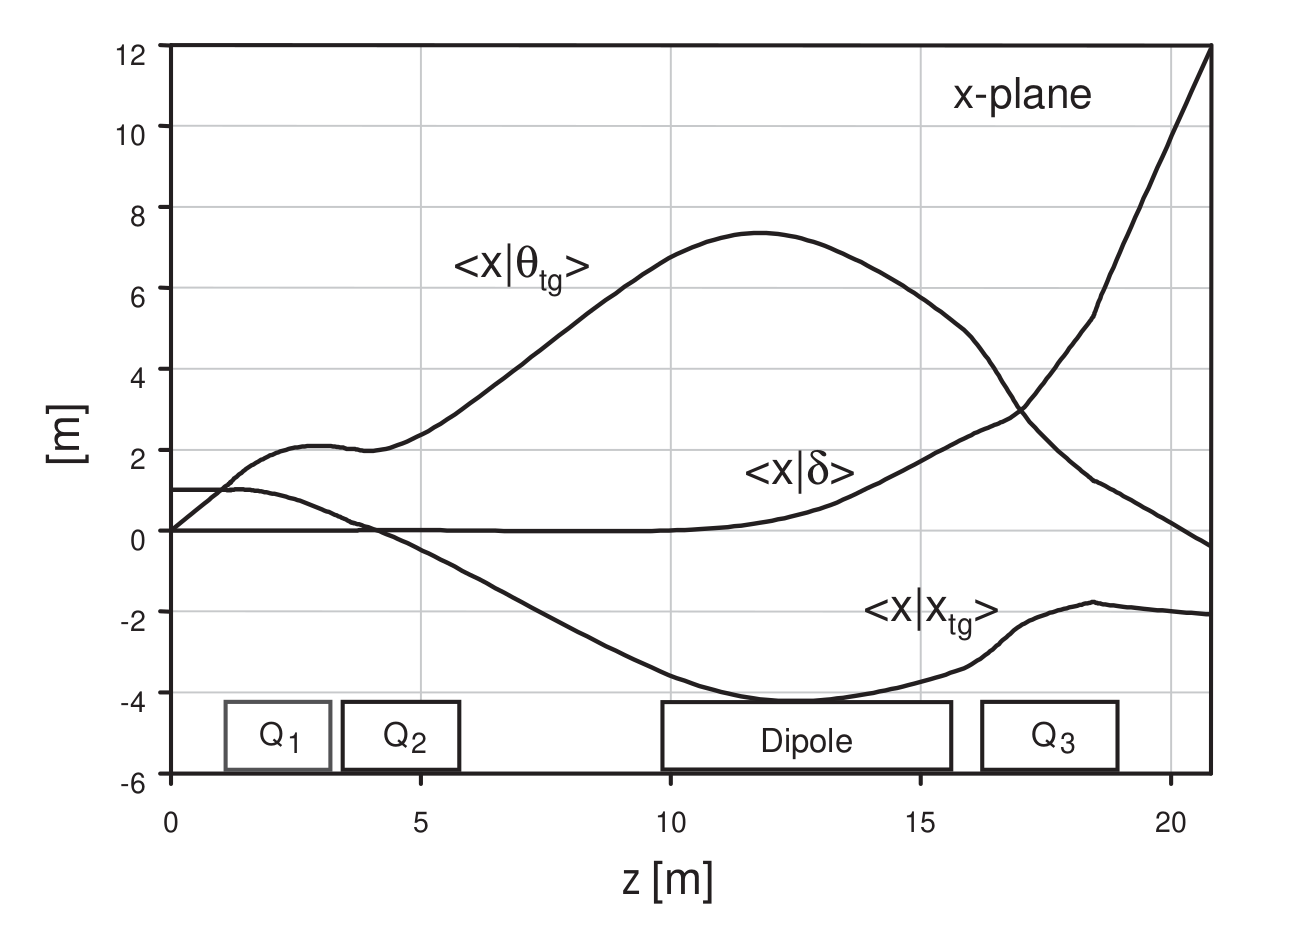
\includegraphics[width=0.50\linewidth]{hrs_transport_x}
    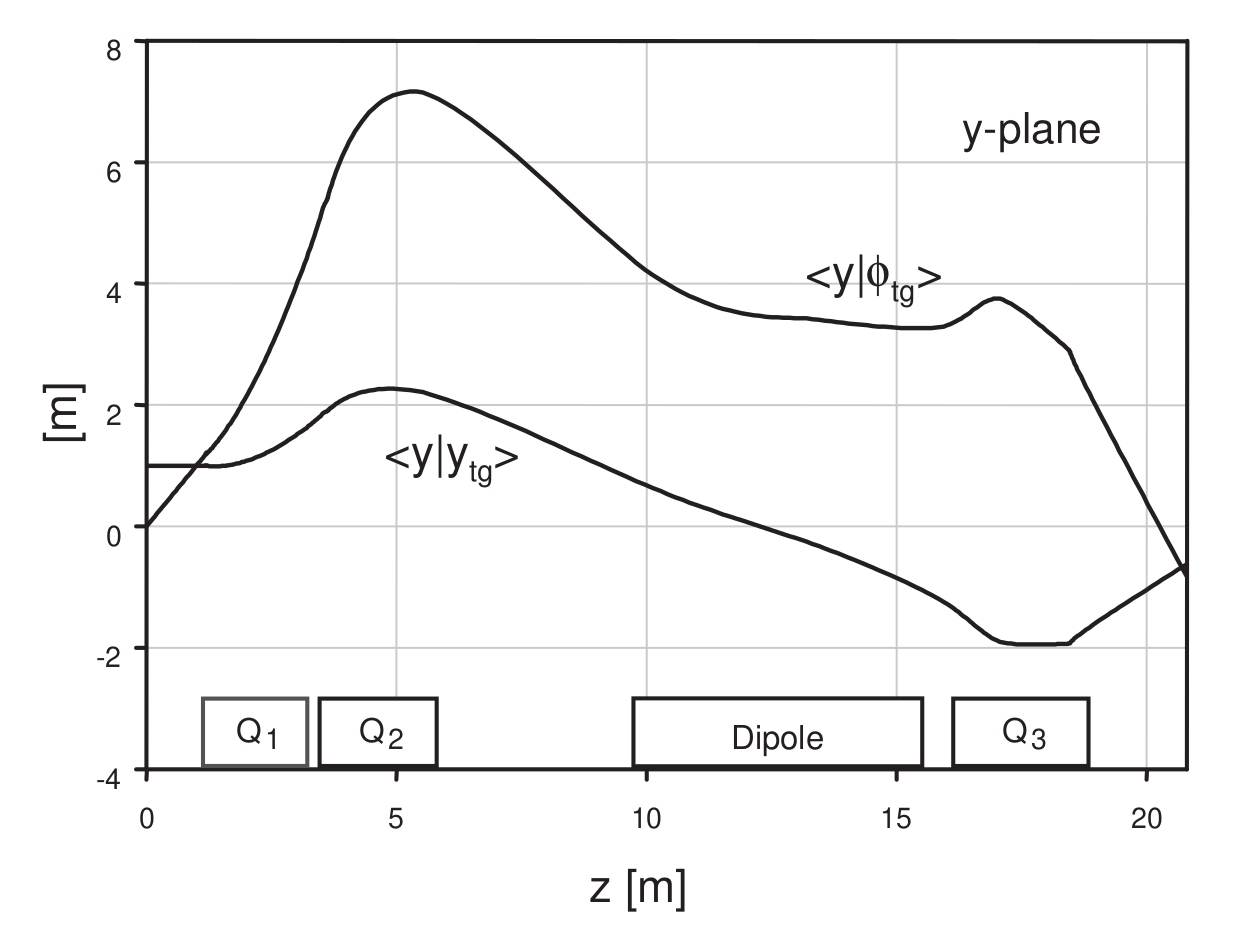
\includegraphics[width=0.48\linewidth]{hrs_transport_y}
    \caption{Transportation plot of HRS. One can clearly see the dispersion effect
    due to shift in momentum ($\delta$) in the Dipole area and the convergent effect
    of Q3.}
    \label{fig:hrs_transport}
\end{figure}

Actually, we don't need to measure every element of T, some elements are obviously
0. E.x. $\delta$ should be not be changed by any magnetic field, so $T_{5i, i\ne 5} = 0$.
The design of HRS tells us that the dispersion depends only on $\delta$, but not
on $\theta$ or $\phi$, so $x|\theta = 0$. Different planes should not
interfere with each other, so that $x|y = x|\phi = \theta|y = \theta|\phi 
= y|x = y|\theta = \phi|x = \phi|\theta = 0$. This is a sparse matrix.

The matrix elements were measured using beam trajectory with sieve slit collimator
inserted in. When the sieve slit collimator was put in, the electron trajectory
from different holes were naturally separated on the focal plane, which allowed
us to match them to sieve holes one by one. With a reasonable initial value of 
the transportation matrix (from previous experiments),
we could reconstruct electron's trajectory on the sieve plane using Eq.~\ref{eq:reconstruction}.
By tuning the matrix element, the one that minimizes the distance of each electron's trajectory on the sieve
plane from its corresponding hole center was identified as the transportation
matrix, so this is a linear regression problem. The identification of the septum 
and HRS current was based on the sieve pattern calculated from the 
transportation matrix. 

% The transportation matrix was extracted for following optics runs:
% \begin{table}
%     \centering
% \end{table}
% what's the difference between PREX-II and CREX?
% how many non-zero elements on the initial matrix?
% which run was used? how different runs/number of effects affect the final result
% energy on the quartz plane:

%%%%%%%%%%%%%%%%%%%%%%%%%%%%%%%%%%%%%%%%%%%%%%%%
\subsection{Scattering Angle $\theta_{lab}$}
The parameter that directly reflects the quality of simulation is the scattering
angle, while it was more convenient to use the Target Coordinate System (TCS) 
than the Hall Coordinate System (HCS) in simulation, we finally were comparing
the scattering angle in the lab frame. The 2 coordinate systems and the transportation
between them are defined below.

\begin{itemize}
    \item Hall Coordinate System: originated at the center of the hall and
	cross the beam line.  $\hat{Z}$ is along the beam line, pointing downstream; 
	$\hat{y}$ points up and $\hat{x}$ points left to form a RH coordinate system.
    \item Target Coordinate System: each HRS specific, the transport coordinate at target position.
	$\hat{z}$ is along the beam trajectory, pointing away the target, 
	$\hat{x}$ in the dispersive plane and points down, $\hat{y}$ is perpendicular
	to the dispersive plane and points away (toward) the beamline for L-HRS (R-HRS).
\end{itemize}

\begin{figure}[H]
    \begin{subfigure}[b]{0.5\textwidth}
	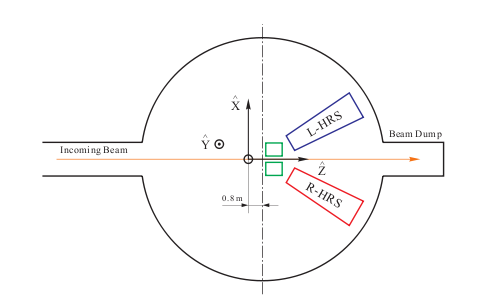
\includegraphics[width=\linewidth]{HCS}
	\caption{Top view of HCS}
    \end{subfigure}
    \begin{subfigure}[b]{0.5\textwidth}
	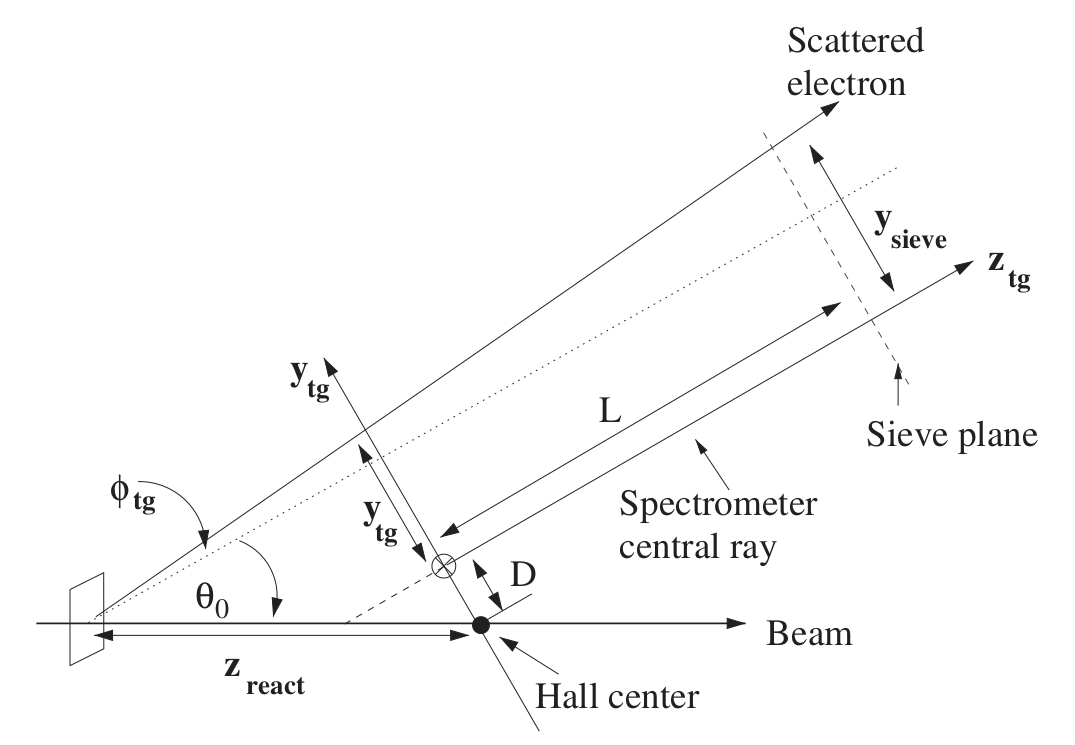
\includegraphics[width=\linewidth]{TCS}
	\caption{Top view of TCS}
    \end{subfigure}
    \caption{Schematic plot of HCS and TCS. The Hall center is the origin of the 
    HCS, but the target doesn't necessary lie in the Hall center. The distance
    from the Hall center to the sieve plane L is constant, which is used to
    identify the origin of the TCS. In ideal case, the origins of both coordinate
    systems will overlap.}
\end{figure}

The relationship between HCS and TCS is:
\begin{equation}
    \begin{pmatrix}
	x_{tg}	\\
	y_{tg}	\\
	z_{tg}	\\
    \end{pmatrix}
    =
    \begin{pmatrix}
	\cos(90^\circ)   & -\sin(90^\circ)    & 0	\\
	\sin(90^\circ)   & \cos(90^\circ)     & 0	\\
	0   & 0     & 1	\\
    \end{pmatrix}
    \begin{pmatrix}
	\cos(-\theta_0)	& 0 & -\sin(-\theta_0)  \\
	0		& 1 & 0		\\
	\sin(-\theta_0)	& 0 & \cos(-\theta_0)  \\
    \end{pmatrix}
    \begin{pmatrix}
	x   \\
	y   \\
	z   \\
    \end{pmatrix}
\end{equation}

\begin{equation}
    \left.
    \begin{aligned}
	x_{tg}	&= -y	\\
	y_{tg}	&= x\cos\theta_0 + z\sin\theta_0    \\
	z_{tg}	&= -x\sin\theta_0 + z\cos\theta_0   \\
    \end{aligned}
    \right\}
    \iff
    \left\{
    \begin{aligned}
	x   &= y_{tg}\cos\theta_0 + z_{tg}\sin\theta_0	\\
	y   &= -x_{tg}	\\
	z   &= -y_{tg}\sin\theta_0 + z_{tg}\cos\theta_0   \\
    \end{aligned}
    \right.
\end{equation}
Define $R = \left(x^2 + y^2 + z^2\right)^{1/2} = z_{tg} \left(\phi^2_{tg} + \theta^2_{tg} + 1\right)^{1/2}$.
So the scattering angle in the lab frame will be:
\begin{equation}
    \cos\theta = \frac{z}{R} = \frac{-\phi_{tg}\sin\theta_0 + \cos\theta_0}{\left(\phi^2_{tg} + \theta^2_{tg} + 1\right)^{1/2}}
\end{equation}
For data, $\theta_0$ was identified to be $4.789^\circ$ ($4.771^\circ$) for
L-HRS (R-HRS). In simulation, both arms used $4.74^\circ$. Note that $\theta_{lab}$
is a post-target (apparent) quantity, which includes effect of post-vertex radiation and
multi-scattering, not the `real' scattering angle (vertex quantity) at the vertex 
where the interesting PV elastic scattering happens. The correction from the apparent 
distribution to the vertex distribution is about 1.5\%.
\begin{figure}[H]
    \centering
    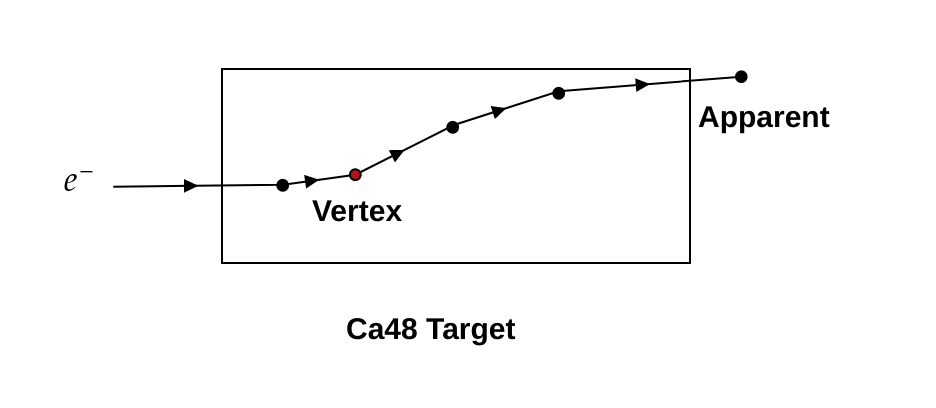
\includegraphics[width=0.5\linewidth]{scattering}
    \caption{Schematic plot of vertex and apparent quantities.}
\end{figure}

%%%%%%%%%%%%%%%%%%%%%%%%%%%%%%%%%%%%%%%%%%%%%%%%
\subsection{Data}
\begin{table}[h!]
    \begin{tabular}{c c | c | c | c c c c}
	\hline
	Exp & Arm   & Dipole p0 ($GeV$)    & Septum ($A$)  & Q1 ($A$)	& A2 ($A$) & Q3 ($A$)  \\
	\hline
	\multirow{2}{*}{PREX-II} & Left	& 0.95285   & 333   & 118.50	& 407.70    & 450.76    \\
				 & Right& 0.95284   & 333   & 118.55	& 404.07    & 446.90    \\
	\hline
	\multirow{2}{*}{CREX}	& Left	& 2.183522  & 801   & 225.387	& 934.273   & 981.301    \\
				& Right	& 2.183499  & 801   & 230.916	& 925.955   & 981.301    \\
	\hline
    \end{tabular}
    \caption{PREX-II and CREX tune}
    \label{tab:pcrex_tune}
\end{table}

\begin{comment}
    PREX tune B: p7 in https://prex.jlab.org/DocDB/0001/000112/001/OpticsCalc.pdf
    \begin{equation}
	\begin{pmatrix}
	    x_{fp}  \\
	    \theta_{fp}  \\
	    y_{fp}  \\
	    \phi_{fp}  \\
	    \delta_{fp}  \\
	\end{pmatrix}
	=
	\begin{pmatrix}
	    -3.09   & -0.02 & 0	& 0 & 16.73 \\
	    -0.31   & -0.32 & 0	& 0 & 2.5   \\
	    0	& 0 & 2.11  & 0.01  & -0.48 \\
	    0	& 0 & 1.1   & 0.48  & -0.19 \\
	    0	& 0 & 0	& 0 & 1	\\
	\end{pmatrix}
	\begin{pmatrix}
	    x_{tg}  \\
	    \theta_{tg}  \\
	    y_{tg}  \\
	    \phi_{tg}  \\
	    \delta_{tg}  \\
	\end{pmatrix}
    \end{equation}
\end{comment}

To determine the new tune of septum and HRS settings for CREX, we started with 
PREX-II tune, scaled it to CREX momentum. To know the appropriate septum 
current that will bridge the central ray into HRS axis we tuned septum and 
Q1 current in 2 steps: coarse and fine tuning. During coarse tuning, we
changed septum and Q1 current by a large step: 10\% (\textbf{central ray search});
and then fine tuned the septum current in a smaller step: 2.5\% to find out
the largest acceptance (\textbf{inner edge search}).

During the central ray search, if the septum current was inappropriate, 
then when we changed the Q1 current, the central hole in reconstructed sieve 
pattern plot would shift, as shown in Fig. \ref{fig:central_ray_0}.
\begin{figure}[H]
    \centering
    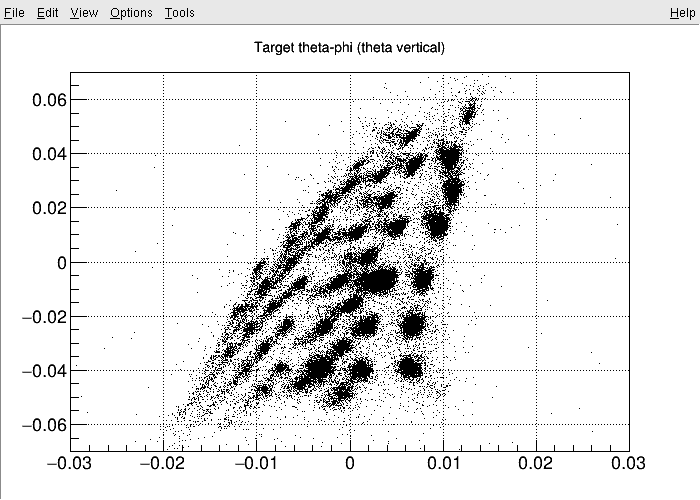
\includegraphics[width=0.32\linewidth]{minus10_septum_minus10_Q1_right}
    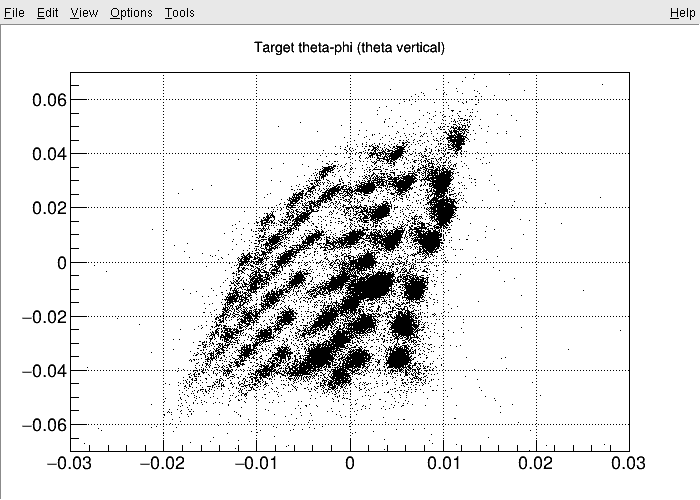
\includegraphics[width=0.32\linewidth]{minus10_septum_nominal_Q1_right}
    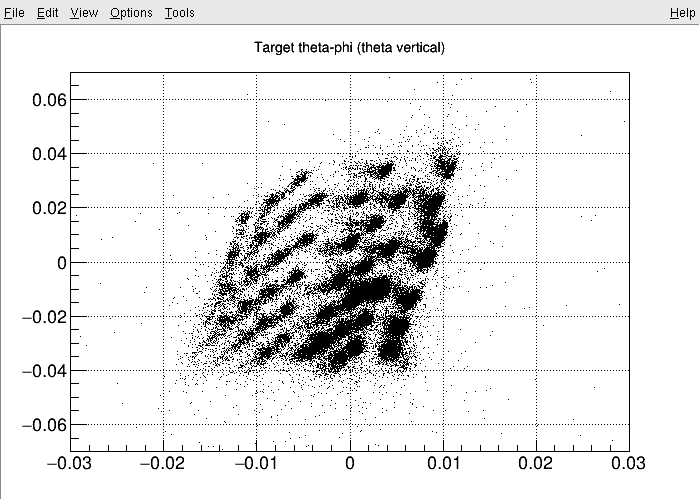
\includegraphics[width=0.32\linewidth]{minus10_septum_plus10_Q1_right}
    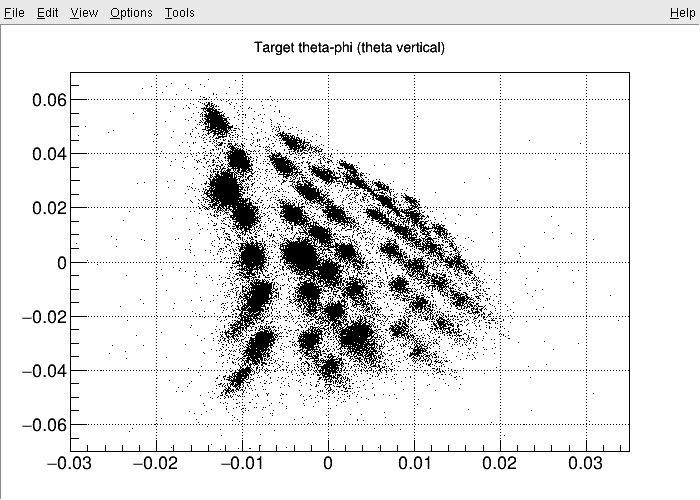
\includegraphics[width=0.32\linewidth]{minus10_septum_minus10_Q1_left}
    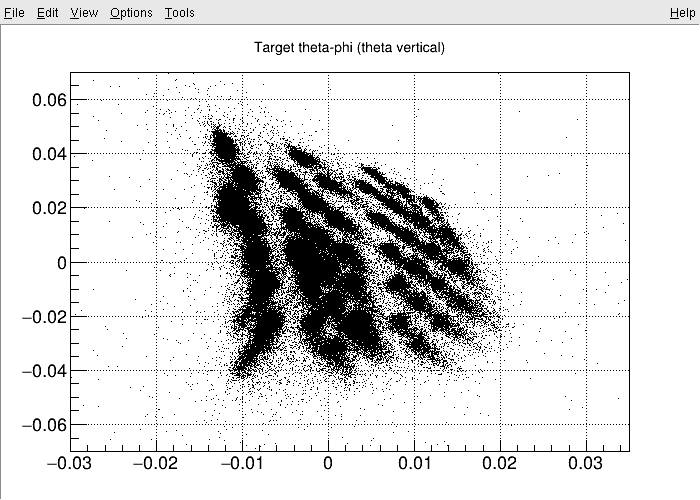
\includegraphics[width=0.32\linewidth]{minus10_septum_nominal_Q1_left}
    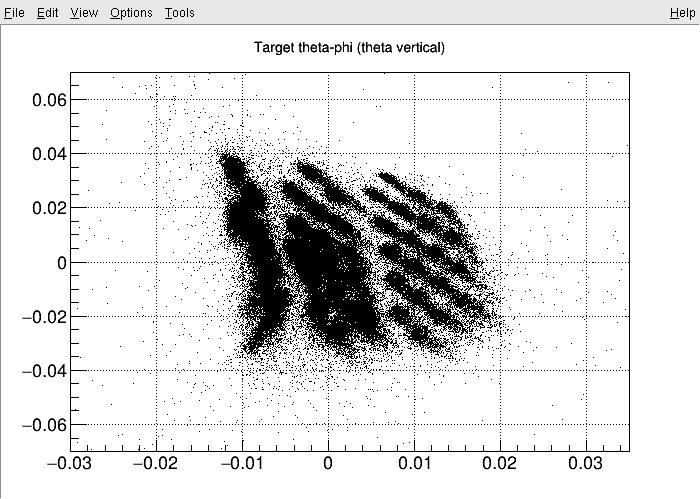
\includegraphics[width=0.32\linewidth]{minus10_septum_plus10_Q1_left}
    \caption{Sieve pattern plots for -10\% septum current
    and varied Q1 current, from left to right: -10\%, nominal and +10\% Q1 current.
    With different Q1 current, the sieve pattern twist, and the central hole 
    shifts in $\theta$, so the septum current is not a good value.}
    \label{fig:central_ray_0}
\end{figure}

\begin{figure}[H]
    \centering
    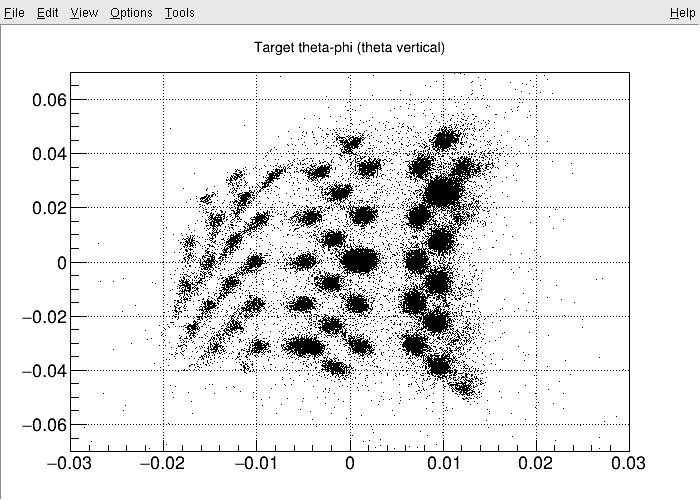
\includegraphics[width=0.32\linewidth]{nominal_septum_minus10_Q1_right}
    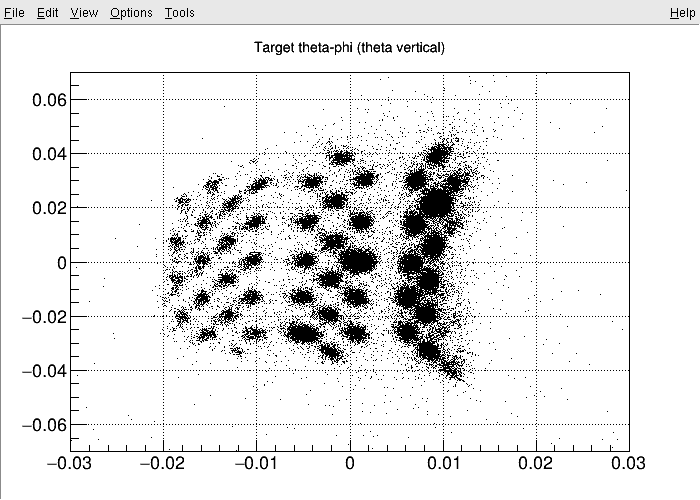
\includegraphics[width=0.32\linewidth]{nominal_septum_nominal_Q1_right}
    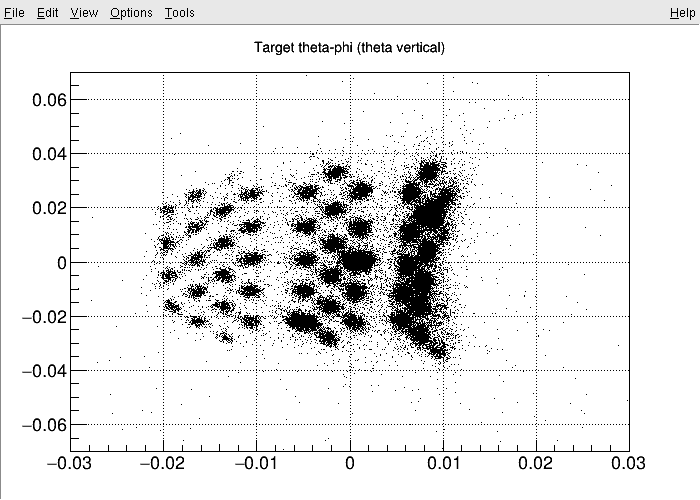
\includegraphics[width=0.32\linewidth]{nominal_septum_plus10_Q1_right}
    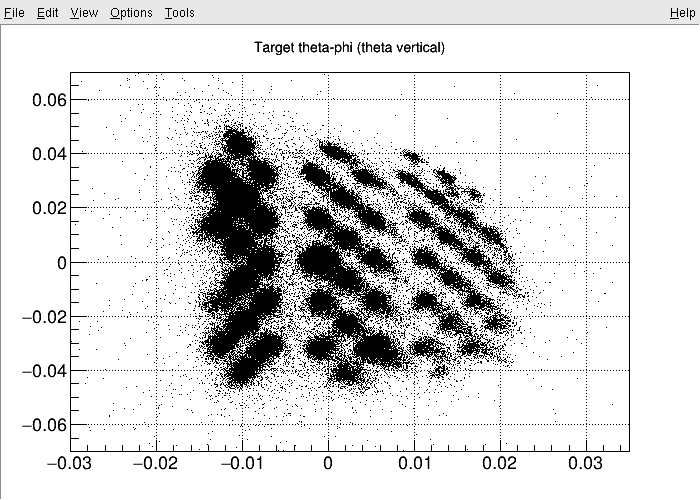
\includegraphics[width=0.32\linewidth]{nominal_septum_minus10_Q1_left}
    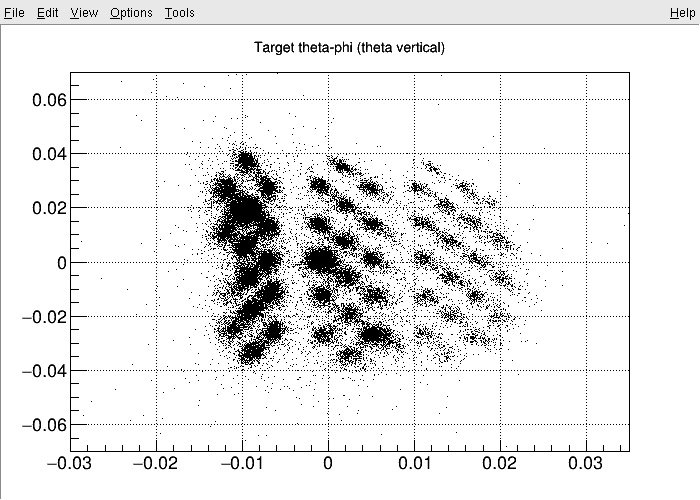
\includegraphics[width=0.32\linewidth]{nominal_septum_nominal_Q1_left}
    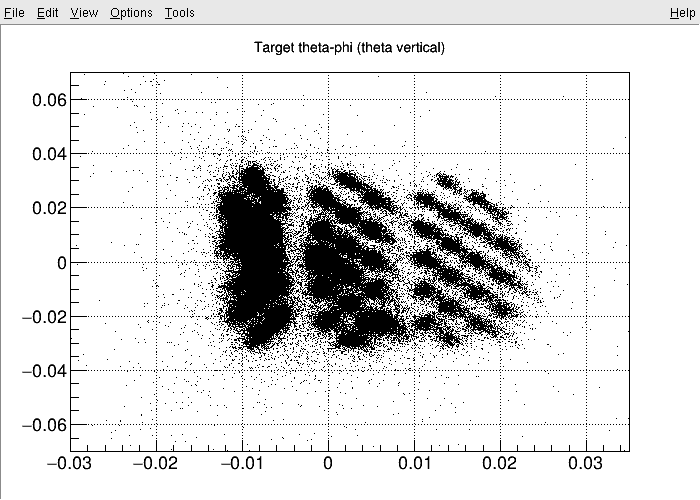
\includegraphics[width=0.32\linewidth]{nominal_septum_plus10_Q1_left}
    \caption{Sieve pattern plots for nominal (scaled from PREX-II setting) septum current
    and varied Q1 current, from left to right: -10\%, nominal and +10\% Q1 current.
    Top row is right arm and bottom row is left arm. With different Q1 current,
    the sieve pattern twist, but the central hole keeps at the same position, 
    which means the central ray goes through the axis of the HRS.}
    \label{fig:central_ray_1}
\end{figure}

Fig. \ref{fig:central_ray_1} told us the nominal septum current and HRS settings was not a bad choice,
so we could move on to inner edge search with this septum nominal value: to
see more inner holes -- holes with largest (smallest) phi in Left (right) arm.
It turned out a 5\% increment from the nominal value gave us the largest 
acceptance, which corresponds to a septum current of: $1.05 \times (333*2.183522/0.95285) = 801.25 \ A$.
\begin{figure}[H]
% https://logbooks.jlab.org/entry/3748464
    \begin{tikzpicture}
	\begin{scope}
	    \node[anchor=south west, inner sep=0] (image) at (0, 0)
	    {	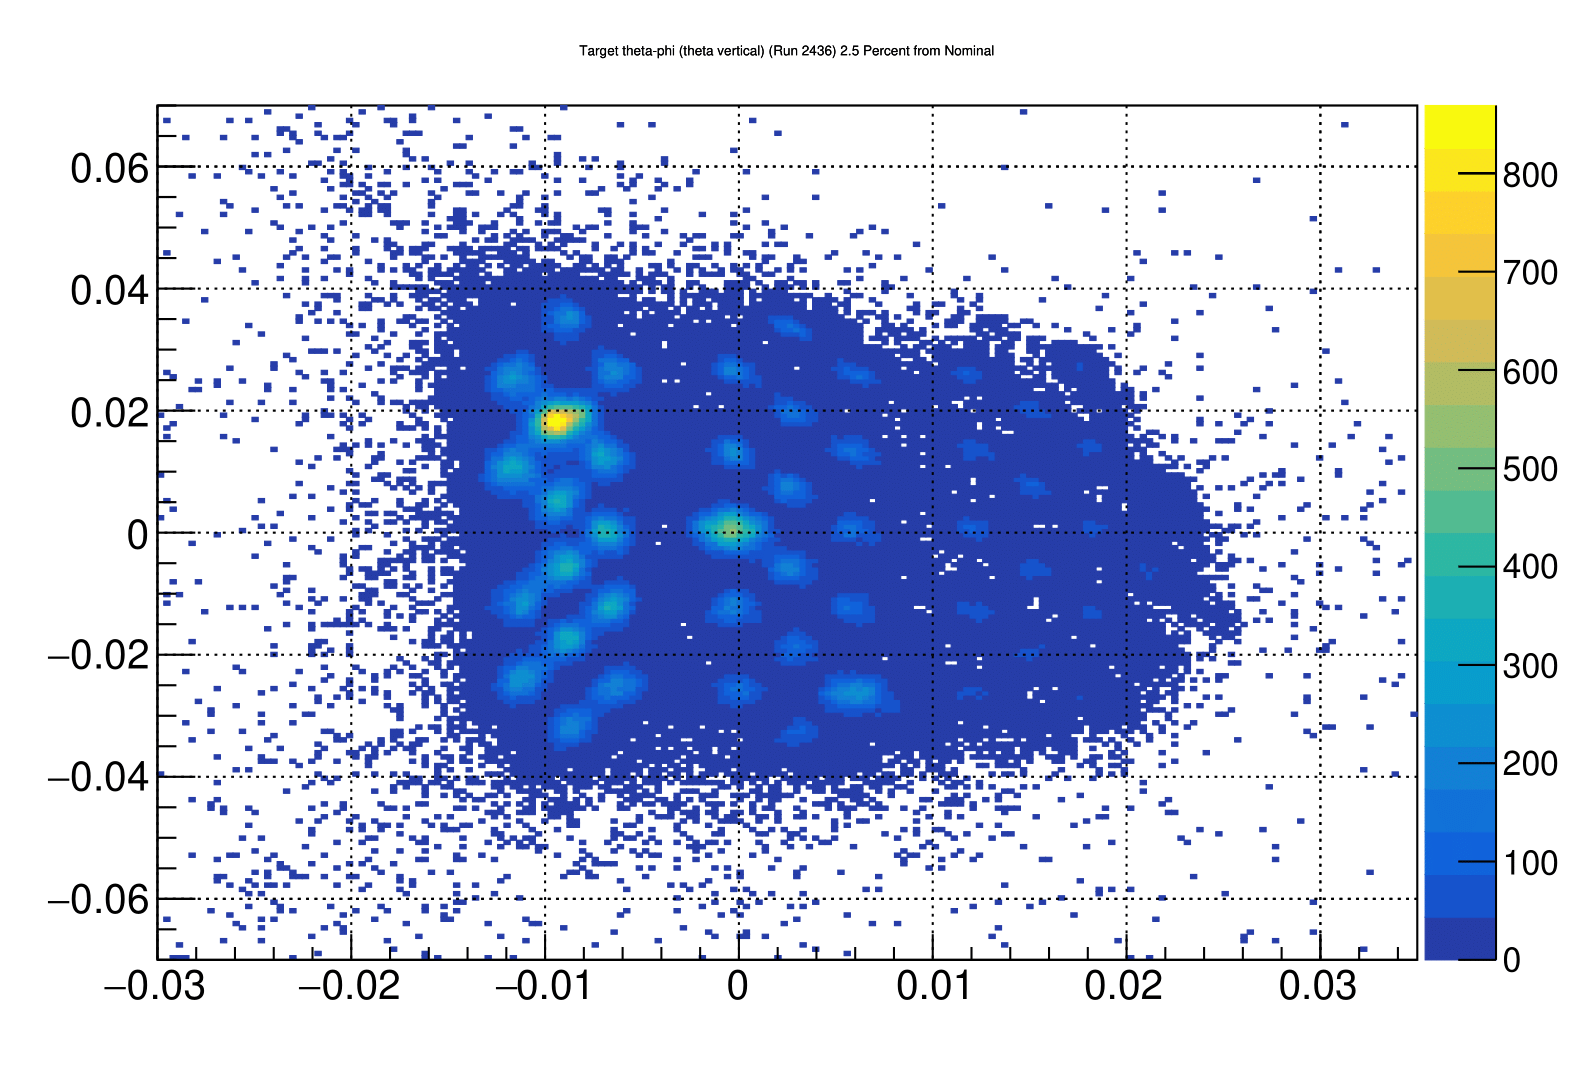
\includegraphics[width=0.49\linewidth]{plus2.5_septum} 
		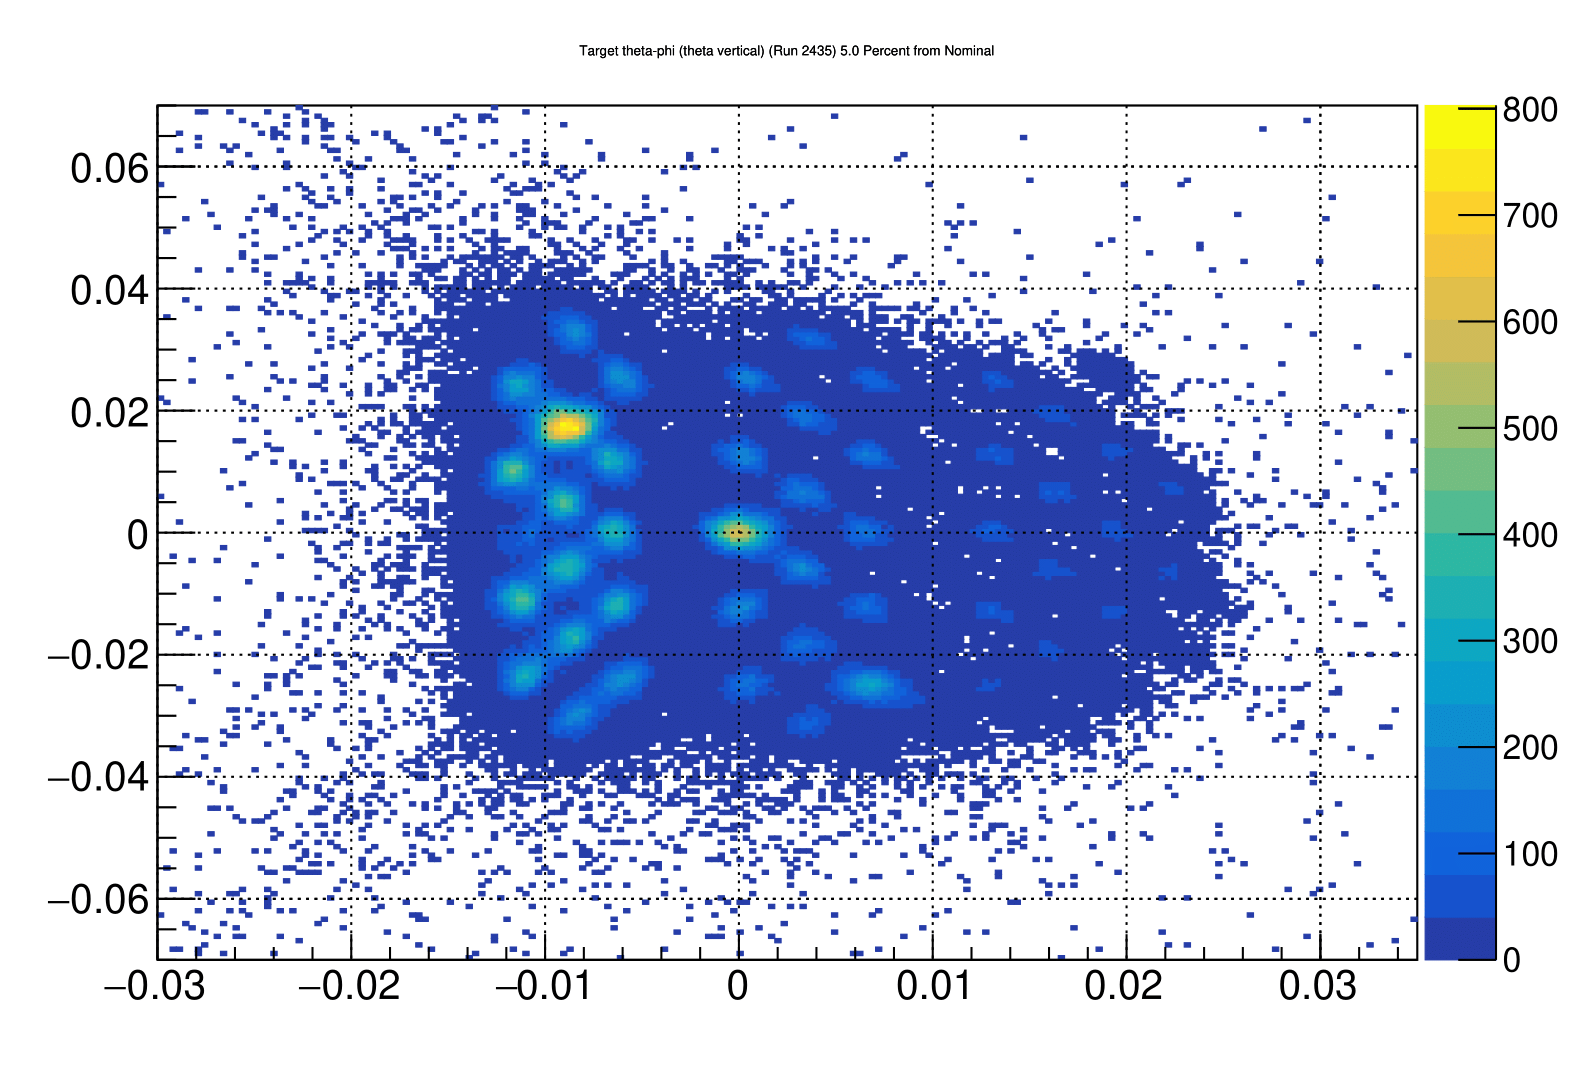
\includegraphics[width=0.49\linewidth]{plus5_septum} 
	    };
	    \begin{scope}[x={(image.south east)}, y={(image.north west)}]
		\draw [thick, Red] (0.67, 0.5) circle (4 pt);
		\draw [thick, Yellow] (0.874, 0.46) circle (4 pt);
		\draw [thick, Yellow] (0.874, 0.55) circle (4 pt);
	    \end{scope}
	\end{scope}
    \end{tikzpicture}
    \begin{tikzpicture}
	\begin{scope}
	    \node[anchor=south west, inner sep=0] (image) at (0, 0)
	    {	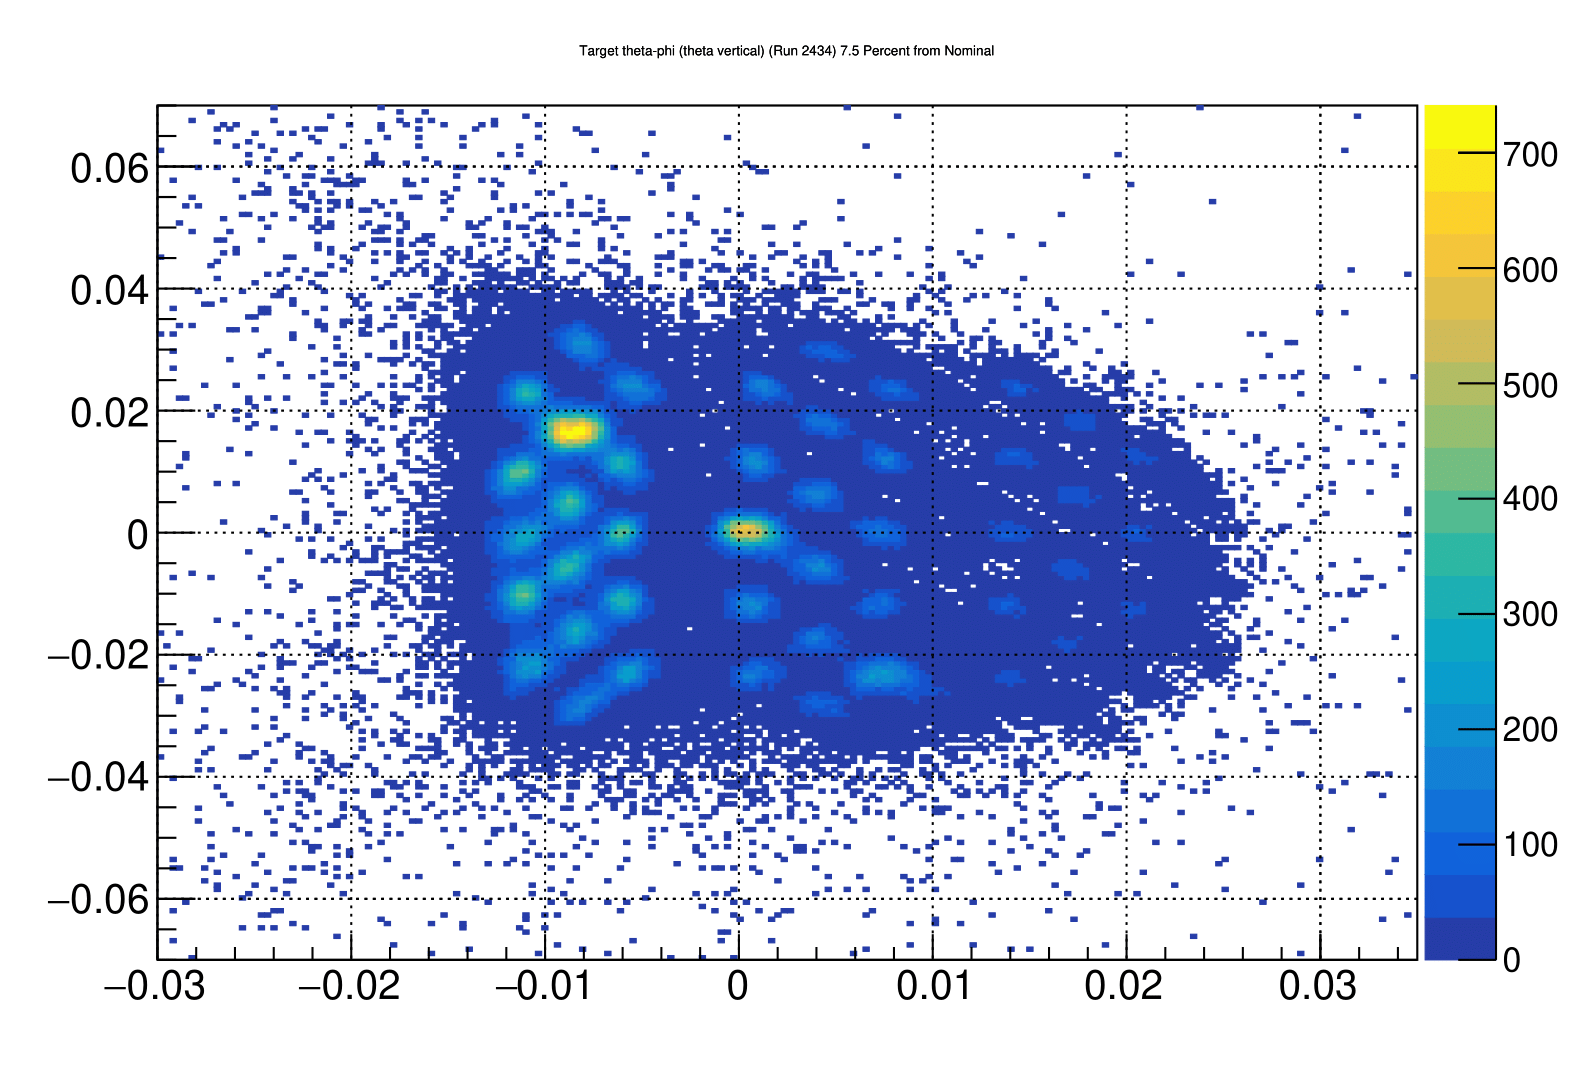
\includegraphics[width=0.49\linewidth]{plus7.5_septum} 
		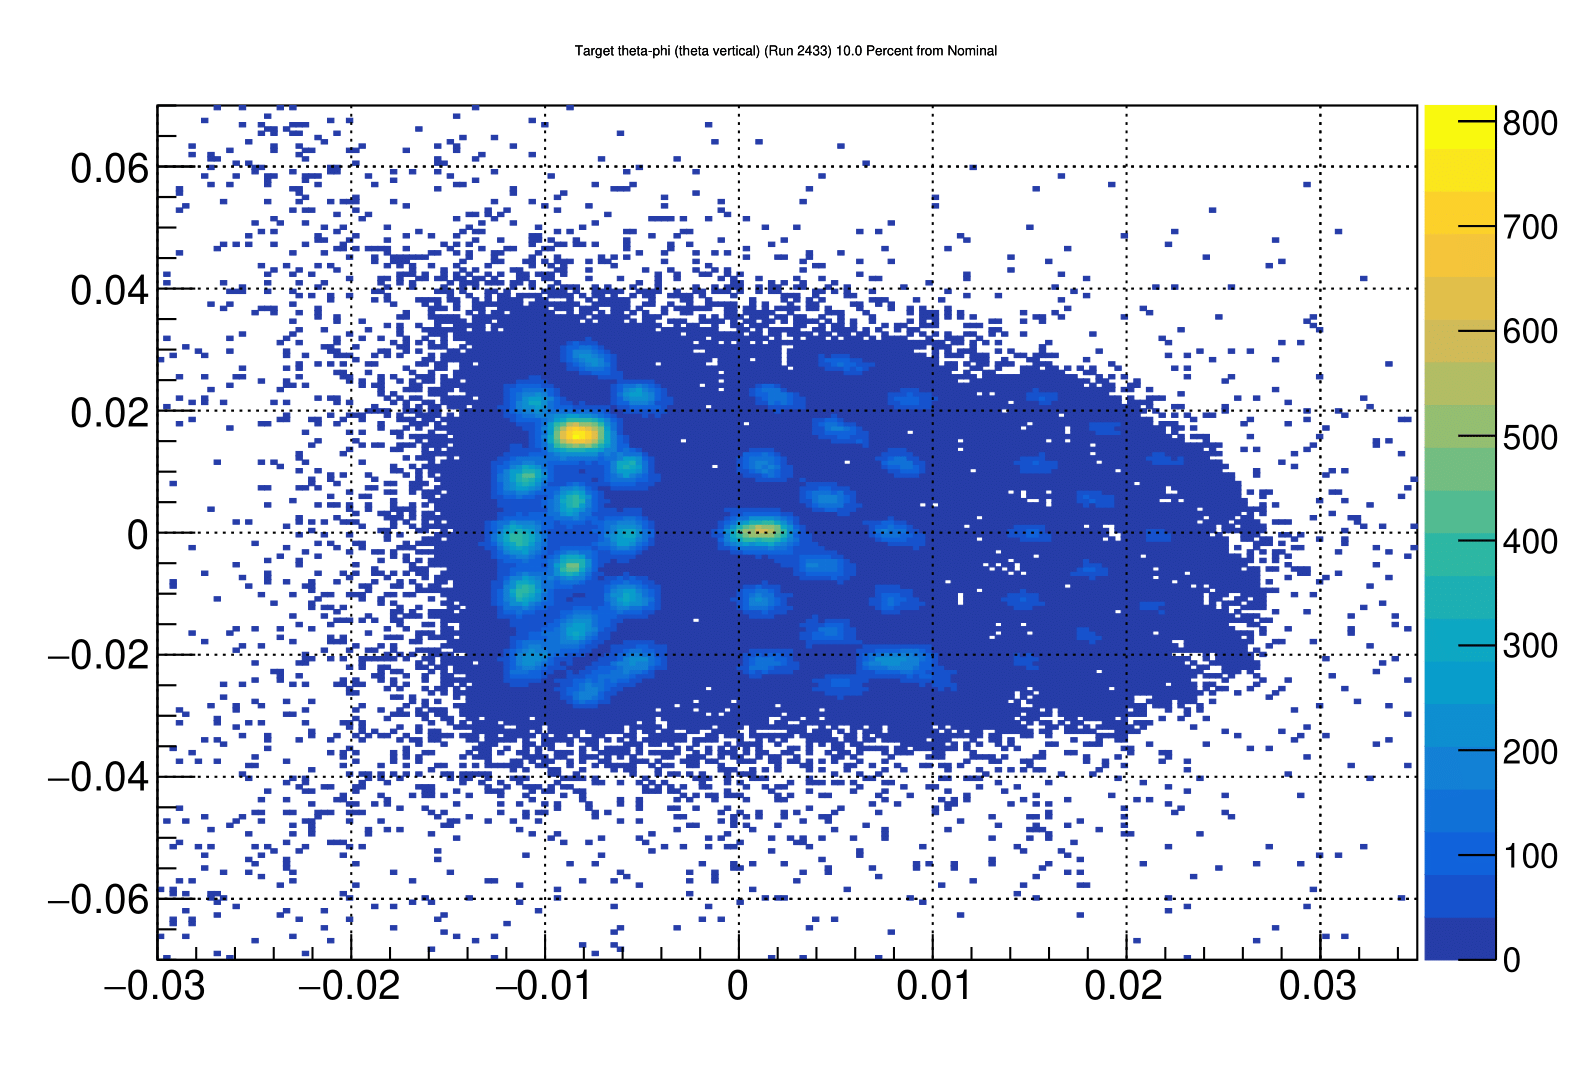
\includegraphics[width=0.49\linewidth]{plus10_septum} 
	    };
	\end{scope}
    \end{tikzpicture}
    \caption{Inner edge search on the left arm. Septum current from top left
    to bottom right: +2.5\%, +5\%, +7.5\%, +10\%. The inner middle hole starts
    to appear since +5\%, and outer holes disappear since 7.5\%, so the best
    septum current was chosen to be +5\%}
\end{figure}

With selected septum current, we continued to minimize beam spot size on the detector
plane, a fine tune of Q1 and Q3 gave us the smallest detector spot size with
Q1 -17\% (-15\%) from the nominal value on left (right) arm, and Q3 -5\% from
the nominal value on both arms, which led to the final CREX tune as shown in
Table~\ref{tab:pcrex_tune}.
\begin{table}[h!]
    \begin{tabular}{c c | c c c | c c c}
	\hline
	& & \multicolumn{3}{c}{Left} & \multicolumn{3}{c}{Right}  \\
	\hline
	Q1(\%)  & Q3 (\%)    & run   & $\sigma_y\ (cm)$  & $\sigma_x\ (cm)$   & run   & $\sigma_y\ (cm)$    & $\sigma_x\ (cm)$    \\
	\hline
	0   & 0	    & 2524  & 0.9604	& 1.634	    & 21604	& 0.009564  & 0.01503 \\
	-5  & 0	    & 2525  & 0.955	& 1.188	    & \multicolumn{3}{c}{Left arm only}    \\
	-10 & 0	    & 2526  & 1.005	& 0.9063    & \multicolumn{3}{c}{Left arm only}    \\ 
	-15 & 0	    & 2527  & 0.1078	& 0.7314    & \multicolumn{3}{c}{Left arm only}    \\ 
	-20 & 0	    & 2528  & 1.182	& 0.6801    & \multicolumn{3}{c}{Left arm only}    \\ 
	\hline                              
	-11 & 0	    & 2529  & 1.012	& 0.8767    & 21609	& 0.009315  & 0.007337	\\
	-12 & 0	    & 2530  & 1.012	& 0.8349    & 21610	& 0.009429  & 0.006957  \\
	-13 & 0	    & 2531  & 1.033	& 0.7835    & 21611	& 0.009526  & 0.006682  \\
	-14 & 0	    & 2532  & 1.057	& 0.7515    & 21612	& 0.009623  & 0.06367   \\
	\hline                              
	-13 & +10   & 2533  & 1.754	& 1.929	    & 21613	& 0.0162    & 0.0215    \\
	-13 & +5    & 2534  & 1.374	& 0.7282    & 21614	& 0.01276   & 0.01174   \\
	-13 & -5    & 2535  & 0.8357	& 0.9751    & 21615	& 0.008422  & 0.008514  \\
	-13 & -10   & 2536  & 0.8855	& 1.482	    & 21616	& 0.008891  & 0.01387   \\
	\hline
	% -13 & -15   & 2537  & 1.133	& 2.042	    & 21617	& 1.141   & 2.051   \\
	-13 & -2    & 2538  & 0.9415	& 0.8761    & 21618	& 0.9117    & 0.7078  \\
	-13 & -4    & 2539  & 0.8602	& 0.9181    & 21619	& 0.8493    & 0.7912  \\
	-13 & -7    & 2540  & 0.8182	& 1.154	    & 21620	& 0.8304    & 1.027   \\
	-13 & -9    & 2541  & 0.8445	& 1.389	    & 21621	& 0.8545    & 1.268   \\
	-15 & -5    & 2542  & 0.8354	& 0.8869    & 21622	& 0.827	    & 0.7563  \\
	\hline
	-15 (R);-17 (L)	& -5	&2543	& 0.8409	& 0.8315  & 21623 & 0.8382	& 0.7615  \\
	\hline
    \end{tabular}
    \caption{Beam spot size with different HRS settings.}
\end{table}

%%%%%%%%%%%%%%%%%%%%%%%%%%%%%%%%%%%%%%%%%%%%%%%%
\subsection{Simulation}
The simulation was not exactly the reproduction of reality. We used GEANT4 to
simulate the geometry of each component based on the designed values, the
septum magnetic field was scaled from a field map file sampled from the septum
at $j_0 = -1320\ A/cm^2$: % FIXME why?
% https://prex.jlab.org/DocDB/0001/000160/001/g4hrs_tune.pdf
\begin{equation}
    B'_{xyz} = \frac{J}{J_0} \times \frac{P}{P_0} \times B_{xyz}
\end{equation}
The same for HRS field: % how to know HRS field at each position
\begin{equation}
    B'_{i = Q1, Q2, D, Q3} = \frac{P}{P_0} \times B_i
\end{equation}

Using this construction, we could firstly vary the septum current to choose the
one that most matched the data, then scanned through collimator shift and pinch point
shift to select the best model.

\begin{figure}[H]
    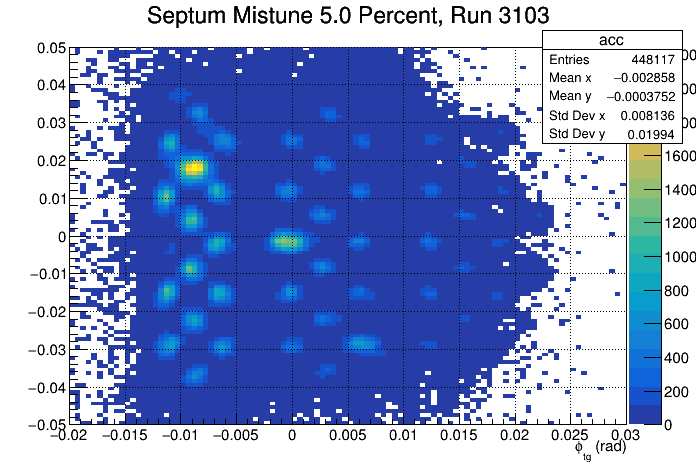
\includegraphics[width=0.49\linewidth]{sieve_run3103}
    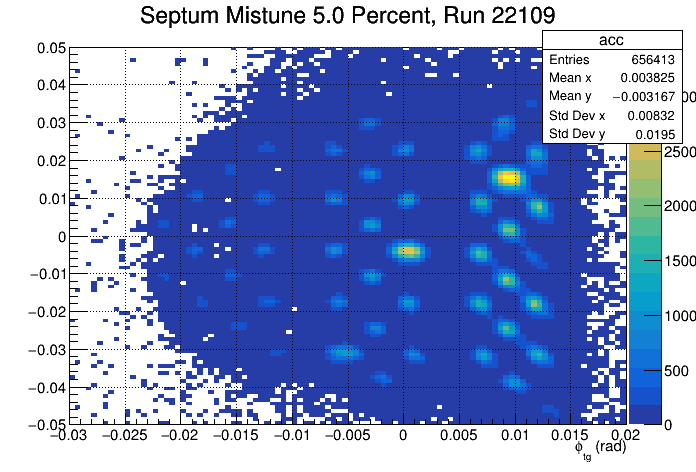
\includegraphics[width=0.49\linewidth]{sieve_run22109}
    \caption{Sieve plot of CREX tune. Centered at (-0.3, -1.5), the new beam 
    position for the new target.}
\end{figure}

Somewhat expected, a coarse scan through the septum told us the septum range
for best model: around 0-5\% above the nominal value.
\begin{figure}[H]
    \begin{tikzpicture}
	\begin{scope}
	    \node[anchor=south west, inner sep=0] (image) at (0, 0)
	    {	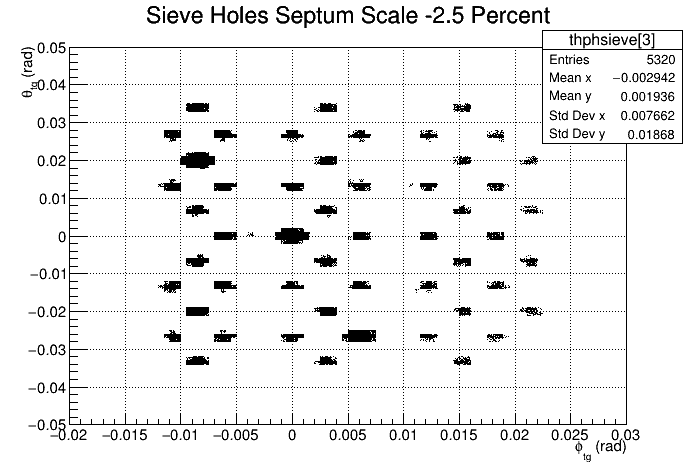
\includegraphics[width=0.49\linewidth]{sieve_sim_minus2.5_left} 
		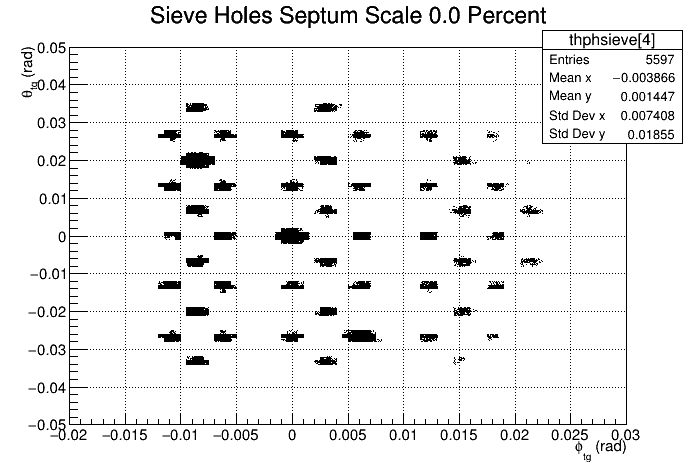
\includegraphics[width=0.49\linewidth]{sieve_sim_nominal_left} 
	    };
	\end{scope}
	\begin{scope}[x={(image.south east)}, y={(image.north west)}]
	    \draw [thick, Red] (0.12, 0.5) circle (4 pt);
	    \draw [thick, Red] (0.33, 0.78) circle (4 pt);
	    \draw [thick, Red] (0.33, 0.23) circle (4 pt);
	    \draw [thick, Red] (0.353, 0.715) circle (4 pt);
	    \draw [thick, Red] (0.353, 0.28) circle (4 pt);
	    \draw [thick, Red] (0.378, 0.655) circle (4 pt);
	    \draw [thick, Red] (0.378, 0.336) circle (4 pt);

	    \draw [thick, Red] (0.83, 0.232) circle (4 pt);
	    \draw [thick, Red] (0.855, 0.715) circle (4 pt);
	    \draw [thick, Red] (0.855, 0.282) circle (4 pt);
	\end{scope}
    \end{tikzpicture}
    \begin{tikzpicture}
	\begin{scope}
	    \node[anchor=south west, inner sep=0] (image) at (0, 0)
	    {	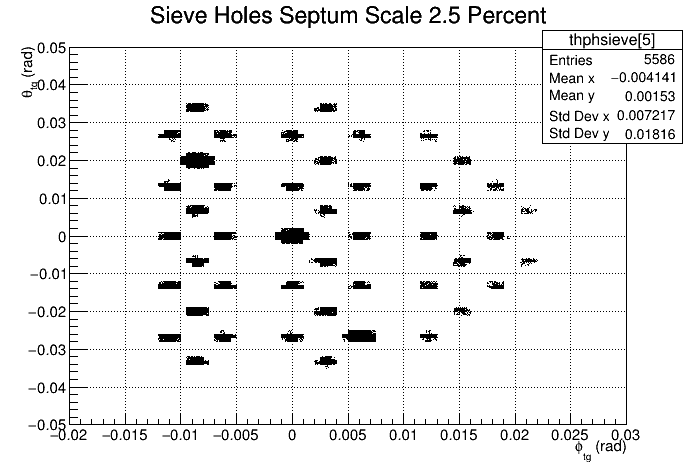
\includegraphics[width=0.49\linewidth]{sieve_sim_plus2.5_left} 
		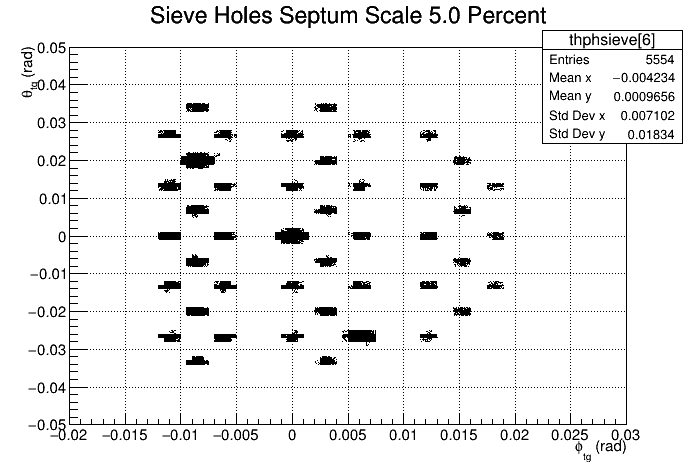
\includegraphics[width=0.49\linewidth]{sieve_sim_plus5_left} 
	    };
	\end{scope}
	\begin{scope}[x={(image.south east)}, y={(image.north west)}]
	    \draw [thick, Red] (0.88, 0.45) circle (4 pt);
	    \draw [thick, Red] (0.88, 0.55) circle (4 pt);
	\end{scope}
    \end{tikzpicture}
    \caption{Sieve pattern plots from simulation with different septum current.}
\end{figure}

\begin{figure}[H]
    \centering
    \begin{tikzpicture}
	\begin{scope}
	    \node[anchor=south west, inner sep=0] (image) at (0, 0)
	    {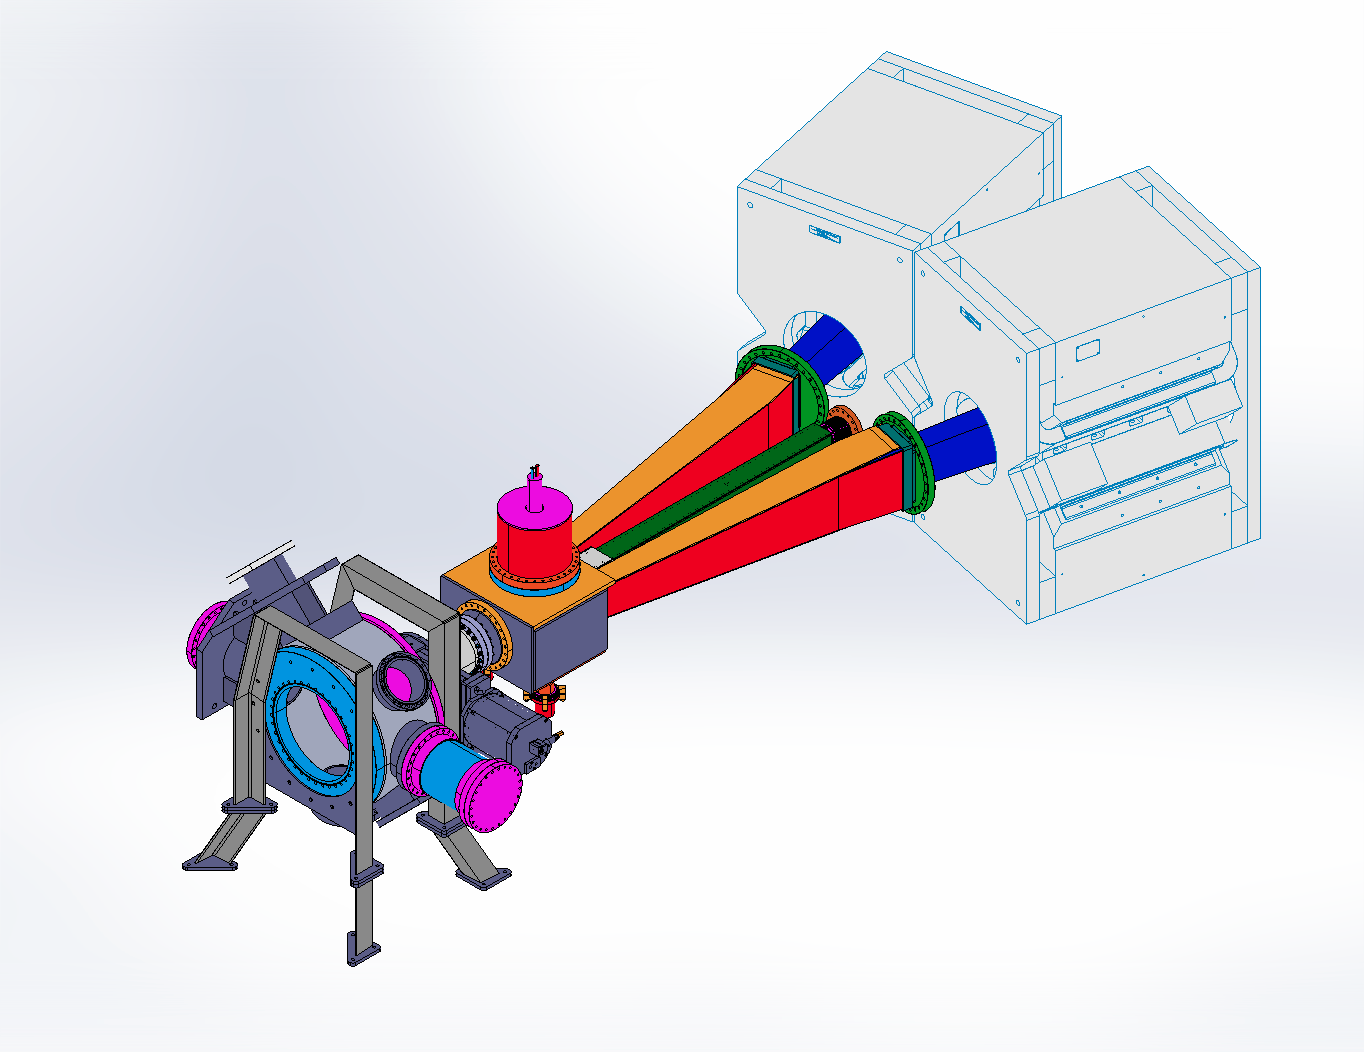
\includegraphics[width=0.5\linewidth]{pivot_region_0}};
	    \begin{scope}[x={(image.south east)},y={(image.north west)}]
		\draw[red,ultra thick] (0.44,0.44) circle (0.17 cm);
		\draw [-latex, thick, red] (0.46, 0.1) node {\scriptsize{Pinch Point}} -- (0.44,0.39);
		\node[green] (coll) at (0.7, 0.2) {\scriptsize{Collimator}};
		\draw [-latex, thick, green] (coll.north) -- (0.67,0.51);
	    \end{scope}
	\end{scope}
    \end{tikzpicture}
    \caption{Position of the pinch point and the Q1 collimator.}
\end{figure}
Then we can scan through the pinch point and collimator shift with a fine tune
of the septum current (from -1\% to +5\%). The pinch point is the connection point
between the septum beampipe and the collimator box, whose misalignment will affect
the acceptance; another parameter we can tune is the collimator (TCS) y position,
which of course has a large impact on the acceptance. For each simulation, we
will compare the average scattering angle $\theta_{lab}$, $Q^2$ and asymmetry to
that of optics data.

\begin{figure}[H]
    \centering
    \includegraphics[width=0.32\linewidth]{pinch_scan_th_lab_-1_run0}
    \includegraphics[width=0.32\linewidth]{pinch_scan_qsq_-1_run0}
    \includegraphics[width=0.32\linewidth]{pinch_scan_asym_-1_run0}
    \includegraphics[width=0.32\linewidth]{pinch_scan_th_lab_2_run99999}
    \includegraphics[width=0.32\linewidth]{pinch_scan_qsq_2_run99999}
    \includegraphics[width=0.32\linewidth]{pinch_scan_asym_2_run99999}
    \caption{Ratio of simulation to data average value for 
    $\theta_{lab}$, $Q^2$ and $\CA$. Top (bottom) row for left (right) arm.
    % FIXME: average over which runs?
    }
    \label{fig:pinch_scan}
\end{figure}

As shown in Fig. \ref{fig:pinch_scan}, when we shift the pinch point toward the
beam pipe (from negative values to positive values for left arm, opposite for 
right arm), the acceptance increases until the nominal value, and then saturates. 
Similar trend was seen for shift of Q1 collimator.
\begin{figure}[H]
    \centering
    \includegraphics[width=0.49\linewidth]{col_scan_th_lab_0_run0}
    \includegraphics[width=0.49\linewidth]{col_scan_th_lab_0_run99999}
\end{figure}

Various correction was applied to the simulation values. That includes the position
difference between the production target and the calibration target, which was
$20\ mm$ downstream the production \Ca target; and the correction caused by
the database, which was optimized on one beam position ($x_0, y_0$):
\begin{equation}
    \phi_a = \phi_r + 0.5\ mrad/mm \times (x - x_0) + 0.5\ mrad/mm \times (y - y_0)
\end{equation}
(x, y) is the actual beam position. $\phi_a$ and $\phi_r$ are actual and reconstructed
$\phi_{tg}$. An extra acceptance was added to the right arm to get a better 
match.

From the ratio plot, we selected the best model which had the smallest difference
between simulation and data in $\theta_{lab}$ and $Q^2$:
\begin{table}[h!]
    \centering
    \begin{tabular}{c | c c c c}
	\hline
	    & septum & col shift ($mm$)	& pinch point shift ($mm$)	\\
	\hline
	LHRS	& +2\%	& -1	& 0 \\
	RHRS	& +5\%	& 2	& 0 \\
	\hline
    \end{tabular}
\end{table}

We can check the $\theta_{lab}$ for the best models
\begin{figure}[H]
    \centering
    \includegraphics[width=0.49\linewidth]{best_model_run2886_th_lab}
    \includegraphics[width=0.49\linewidth]{best_model_run2886_qsq}
    \includegraphics[width=0.49\linewidth]{best_model_run21874_th_lab}
    \includegraphics[width=0.49\linewidth]{best_model_run21874_qsq}
    \caption{$\theta_{lab}$ and $Q^2$ comparison between best models and data (apparent values).}
\end{figure}
% We can also check the difference between the vertex values and data:
% \begin{figure}
%     \centering
%     \includegraphics[width=0.49\linewidth]{p3_-2_0_0.0_run2886_th_lab_v}
%     \includegraphics[width=0.49\linewidth]{p3_-2_0_0.0_run2886_qsq_v}
%     \includegraphics[width=0.49\linewidth]{p5_0_-1_0.0_run21874_th_lab_v}
%     \includegraphics[width=0.49\linewidth]{p5_0_-1_0.0_run21874_qsq_v}
%     \caption{$\theta_{lab}$ and $Q^2$ comparison between best models and data (apparent values).}
% \end{figure}

Using this best models, we can calculate the acceptance function as Eq.~\ref{eq:acceptance_definition}:
\begin{figure}[H]
    \centering
    \includegraphics[width=0.49\linewidth]{acc1_L_p2_-1_0_0.0}
    \includegraphics[width=0.49\linewidth]{acc1_R_p5_2_0_0.0}
    \caption{Acceptance function extracted using the best models.}
\end{figure}

%%%%%%%%%%%%%%%%%%%%%%%%
\subsubsection{Non-Linearity}
\begin{equation}
    Y = I + \alpha I^2 + \beta I^3 + \gamma I^4 + \cdots
\end{equation}
Non-linearity: $\alpha$, reduce it 
\begin{itemize}
    \item $\alpha=0.0028$ for Compton $\gamma$ detector
    % https://prex.jlab.org/DocDB/0002/000273/002/Cornejo_and_Quinn_ComptonPhoton_CREX_PREX_Nov_2018.pdf
\end{itemize}
% \subsection{tg variables}

\chapter{Results and Discussion}

%%%%%%%%%%%%%%%%%%%%%%%%%%%%%%%%%%%%%%%%%%%%%%%%%%%%%%%%%%%%%%%%%%%%%%%%
\section{Final Numbers}
% crex: https://docs.google.com/spreadsheets/d/154c_FlXKs06Dbn1UEjuJeL52RLanBTXx/edit#gid=1377286011

\begin{comment}
    Measured asymmetry 
    $\downarrow$
    correct for Coulomb distortions 
    $\downarrow$
    Weak density at one $Q^2$
    $\downarrow$
    small correction for $G_E^n$, $G_E^s$
    $\downarrow$
    Neutron density at one $Q^2$
    $\downarrow$
    assume surface thickness good to 25\% (MFT)
    $\downarrow$
    $R_n$

\end{comment}
The overall beam polarization is determined by calculating the inverse-variance 
weighted average of the Compton and Moller measurements.
\begin{table}[!h]
    % PREX-II Compton
    % PREX-II Moller: https://prex.jlab.org/DocDB/0004/000468/003/DNP_Oct2020.pdf
    % CREX Compton: AJZ thesis
    % CREX Moller: AJZ thesis
    \centering
    \begin{tabular}{c | c c}
	\hline
	    & PREX-II	& CREX	\\
	\hline
	Compton	& ($89.68 \pm 0.15$)\%  & ($87.115 \pm 0.453$)\%	\\
	Moller	& ($89.67 \pm 0.80$)\%	& ($87.06 \pm 0.74$)\%  \\
	\hline
	Average	& ($89.7 \pm 0.8$)\%	& ($87.10 \pm 0.39$)\%	\\
	\hline
    \end{tabular}
    \caption{Beam polarization measured by the Compton and Moller polarimeters.}
\end{table}

%%%%%%%%%%%%%%%%%%%%%%%%%%%%%%%%%%%%%%%%%%%%%%%%
% \subsection{Asymmetry}
After applying the beam false asymmetry correction described in chapter~\ref{cha:data_analysis} and
identifying various background asymmetries in chapter~\ref{cha:systematic_uncertainties}, 
the blinded PV asymmetry will be extracted using Eq. \ref{eq:background_correction}, 
which we restate here:
\begin{equation*}
    \CA_{\text{PV}} = \frac{\CA_{\text{cor}}/\CP - \sum_i \CA_i f_i}{1 - \sum_i f_i}
\end{equation*}
The list of various corrections to the final result are shown in 
Table~\ref{tab:prex_corrections} and \ref{tab:crex_corrections}.

\begin{table}[!h]
    \centering
    \begin{tabular}{l r@{ $\pm$ }l r@{ $\pm$ }l}
	\hline
	Correction & \multicolumn{2}{c}{Absolute (ppb)}	& \multicolumn{2}{c}{Relative (\%)}   \\
	\hline
	Beam trajectory and energy  & -60.4	& 3.0	& 11.0	& 0.5	\\ 
	Charge correction           & 20.7	& 0.2   & 3.8	& 0.0   \\ 
	\hline
	Beam polarization           & 56.8	& 5.2   & 10.3	& 1.0   \\ 
	Target diamond foils        & 0.7	& 1.4   & 0.1	& 0.3   \\ 
	Spectrometer rescattering   & 0.0	& 0.1   & 0.0  	& 0.0   \\ 
	Inelastic contributions     & 0.0	& 0.1   & 0.0  	& 0.0   \\ 
	Transverse asymmetry        & 0.0	& 0.3   & 0.0  	& 0.1   \\ 
	Detector nonlinearity       & 0.0	& 2.7   & 0.0  	& 0.5   \\ 
	Angle determination         & 0.0	& 3.5   & 0.0  	& 0.6   \\ 
	Acceptance function         & 0.0	& 2.9   & 0.0  	& 0.5   \\ 
	\hline
	Total correction	    & 17.7	& 8.2	& 3.2	& 1.5	\\
	Statistical uncertainty	    & \multicolumn{2}{c}{16}	& \multicolumn{2}{c}{2.9}   \\
	\hline
    \end{tabular}
    \caption{Corrections and corresponding systematic uncertainties to $\CA_{\text{PV}}$ in PREX-II.}
    \label{tab:prex_corrections}
\end{table}

\begin{table}[!h]
    \centering
    \begin{tabular}{l r@{ $\pm$ }l r@{ $\pm$ }l}
	\hline
	Correction & \multicolumn{2}{c}{Absolute (ppb)}	& \multicolumn{2}{c}{Relative (\%)}   \\
	\hline
	Beam trajectory and energy  & 68  & 7     & 2.5	    & 0.3   \\         
	Beam charge asymmetry       & 112 & 1     & 4.2     & 0.0   \\         
	\hline
	Beam polarization	    & 382 & 13    & 14.3    & 0.5   \\         
	Isotopic purity             & 19  & 3     & 0.7     & 0.1   \\         
	3.831 MeV ($2^+$) inelastic & -35 & 19    & -1.3    & 0.7   \\         
	4.507 MeV ($3^-$) inelastic & 0   & 10    & 0	    & 0.4   \\ 
	5.370 MeV ($3^-$) inelastic & -2  & 4     & -0.1    & 0.1   \\         
	Transverse asymmetry        & 0   & 13    & 0	    & 0.5   \\ 
	Detector nonlinearity       & 0   & 7     & 0	    & 0.3   \\         
	Acceptance                  & 0   & 24    & 0  	    & 0.9   \\         
	Radiative corrections	    & 0   & 10    & 0  	    & 0.4   \\         
	\hline
	Total systematic uncertainty	& \multicolumn{2}{c}{40}    & \multicolumn{2}{c}{1.5}	\\
	Statistical uncertainty		& \multicolumn{2}{c}{106}   & \multicolumn{2}{c}{4.0}	\\
	\hline
    \end{tabular}
    \caption{Corrections and corresponding systematic uncertainties to $\CA_{\text{PV}}$ in CREX.}
    \label{tab:crex_corrections}
\end{table}

The last step is unblinding, in which we subtract $\CA_{\text{blind}}$ from the blinded
$\CA_{\text{PV}}$. The blinding factor is a secret value that is randomly generated 
from a $\pm900$~ppb box, this secret value is 
added to each helicity quadruplet (octuplet) asymmetry by the JAPAN analyzer. 
Surprisingly, the value of $\CA_{\text{blind}}$ for PREX-II is very close to 0, 
resulting in the unblinded $\CA_{\text{PV}}$ being almost the same as the blinded value. 
The final asymmetry values are presented in Table~\ref{tab:pcrex_final_number}.
\begin{table}[!h]
    \centering
    \begin{tabular}{c | c c}
	\hline
	Asymmetry   & PREX-II	& CREX	\\
	\hline
	$\CA_{\text{raw}}$ & $431.64 \pm 44.01$    & $2106 \pm 178.9$	\\
	$\CA_{\text{cor}}$ & $492.02 \pm 13.52$    & $2080.3 \pm 83.8$	\\
	Blinded $\CA_{\text{PV}}$ & $549.4 \pm 16.1 \pm 8.1$    & $2412.3 \pm 106.1 \pm 38.7$	\\
	$\CA_{\text{blind}}$	& -0.5	& -255.7    \\
	\hline
	Unblinded $\CA_{\text{PV}}$	& $550 \pm 16 \pm 8$	& $2668 \pm 106 \pm 40$	\\
	\hline
    \end{tabular}
    \caption{The path to a physical PV asymmetry. All values are in units of ppb.}
    \label{tab:pcrex_final_number}
\end{table}

%%%%%%%%%%%%%%%%%%%%%%%%%%%%%%%%%%%%%%%%%%%%%%%%
\subsection{Neutron Skin Thickness}
\label{subsec:neutron_skin_thickness}
With the physical PV asymmetry, the weak FF is calculated using Eq.~\ref{eq:asymmetry}.
\begin{equation}
    F_W ({}^{208}\text{Pb}) = 0.368  \pm 0.013 \ (\text{exp}) \pm 0.001 \ (\text{theo})
\end{equation}
Here the experimental uncertainty incorporates both statistical and systematic contributions.

The experimental value of the weak radius is determined from the correlation between the weak radius and PV asymmetry. In the correlation plot, the weak radius corresponding to the measured PV asymmetry is obtained as the experimental value. Similarly, the neutron skin thickness is derived using the same approach.

The correlation plot is generated by fitting the weak charge densities, which are
predicted by a wide range of DFT models, to a two-parameter Fermi function. 
By knowing the weak charge density function, the corresponding PV asymmetry and
weak radius can be identified for each model, as shown in Fig.~\ref{fig:prex_Rw}.
The two-parameter Fermi function has been discussed in Sec.~\ref{subsec:models}.
\begin{equation*}
    \rho_W(r) = \rho_W^0 \frac{\sinh(c/a)}{\cosh(r/a) + \cosh(c/a)}
\end{equation*}
here $c$ denotes the nuclear size and $a$ describes the surface thickness. 

\begin{figure}[!h]
    \centering
    \includegraphics[width=0.6\linewidth]{prex_Rw}
    \caption[Correlation between the weak radius/neutron skin thickness and $\CA_{\text{PV}}$]
    {Correlation between the weak radius (left vertical axis) or neutron skin thickness 
    (right vertical axis) and $\CA_{\text{PV}}$ for \Pb, as predicted by a series 
    of DFT models \cite{PhysRevLett.126.172502}. 
    The red solid line describes the fitted correlation based on the predictions of
    the DFT models, the red dashed line and the green band indicate the 1-$\sigma$ uncertainty 
    for the correlation and measured values, respectively.}
    \label{fig:prex_Rw}
\end{figure}

% The fits suggest \cite{PhysRevLett.126.172503}:
% \begin{equation}
%     a = 0.605 \pm 0.025\ \mathrm{fm}
% \end{equation}

The weak charge radius of \Pb is extracted to be:
\begin{equation}
    % R^2_W = \frac{1}{Q_W} \int r^2 \rho_W(r)d^3r = \frac{3}{5}c^2 + \frac{7}{5}(\pi a)^2
    R_W ({}^{208}\text{Pb}) = 5.795 \pm 0.082 \ (\text{exp}) \pm 0.013 \ (\text{theo})\ \mathrm{fm}
\end{equation}
and the neutron skin thickness of \Pb:
\begin{equation}
    R_{\text{skin}} ({}^{208}\text{Pb}) = R_n - R_p = 0.278 \pm 0.078 \ (\text{exp}) \pm 0.012 \ (\text{theo})\ \mathrm{fm}
\end{equation}

Similarly, the weak radius and neutron skin thickness of \Ca can be extracted,
as summarized in Table~\ref{tab:pcrex_neutron_skin}.
\begin{table}[!h]
    \centering
    \begin{tabular}{l | c c}
	\hline
	Exp	& PREX-II   & CREX  \\
	\hline
	Target	& \Pb	    & \Ca   \\
	$\langle Q^2 \rangle $ ($\mathrm{GeV}^2$)	& $ 0.00616 \pm 0.00005 $   & $0.0297 \pm 0.0002 $  \\
	$\langle \CA_{\text{PV}} \rangle$ (ppb)   & $550 \pm 16 \ (\text{stat}) \pm 8 \ (\text{syst})$	& $2668 \pm 106 \ (\text{stat}) \pm 40 \ (\text{syst})$ \\
	$F_W$	& $0.368 \pm 0.013 \ (\text{exp}) \pm 0.001 \ (\text{theo})$    & $0.1304 \pm 0.0052 \ (\text{stat}) \pm 0.0020 \ (\text{syst})$    \\
	$F_{ch} - F_W$	& $0.041 \pm 0.013 \ (\text{exp}) \pm 0.001 \ (\text{theo})$    & $0.0277 \pm 0.0052 \ (\text{stat}) \pm 0.0020 \ (\text{syst})$    \\
	$R_W$ (fm)	& $5.795 \pm 0.082 \ (\text{exp}) \pm 0.013 \ (\text{theo})$    & $3.640 \pm 0.026 \ (\text{exp}) \pm 0.023 \ (\text{theo})$\\
	$R_n - R_p$ (fm)  & $0.278 \pm 0.078 \ (\text{exp}) \pm 0.012 \ (\text{theo})$	& $0.121 \pm 0.026 \ (\text{exp}) \pm 0.024 \ (\text{theo})$    \\
	% $\rho_W^0$ ($\mathrm{fm}^{-3}$)	& $-0.0798 \pm 0.0038 \ (\text{exp}) \pm 0.0013 \ (\text{theo})$	&   \\
	% $\rho_b^0$ ($\mathrm{fm}^{-3}$)	& $0.1482 \pm 0.0040 $	&   \\
	\hline
    \end{tabular}
    \caption{Physical results extracted from PREX-II and CREX. 
    % The experimental uncertainty in PREX-II   
    }
    \label{tab:pcrex_neutron_skin}
\end{table}

Combining PREX-I and PREX-II results, the weak radius and the neutron skin are 
determined to be:
\begin{equation}
    \begin{gathered}
	R_W({}^{208}\text{Pb}) = 5.800 \pm 0.075\ \mathrm{fm}  \\
	R_{skin}({}^{208}\text{Pb}) = 0.283 \pm 0.71\ \mathrm{fm}   \\
    \end{gathered}
\end{equation}
%%%%%%%%%%%%%%%%%%%%%%%%%%%%%%%%%%%%%%%%%%%%%%%%
\subsection{Density Dependence of the Symmetry Energy}
In nuclear density functional theory, the neutron skin thickness of \Pb is 
correlated with the density dependence of the symmetry energy $L$. 
By plotting the predictions from DFT calculations using a set of energy density 
functionals, a linear correlation between $L$ and $R_{\text{skin}}$ can be established,
as demonstrated in Fig.~\ref{fig:L_vs_R_skin}. Using this correlation, we can determine
the symmetry energy slope $L$ that corresponds to our measured $R_{\text{skin}}$ in \Pb. 
The values of $L$ at the nuclear saturation density 
$\rho_0 \sim 0.15 \mathrm{fm}^{-3}$ and the nuclear density $\rho_1 \sim 0.15 \mathrm{fm}^{-3}$ 
are determined to be:
\begin{equation}
    L(\rho_0) = 106 \pm 37 \ \mathrm{MeV}	\qquad L(\rho_1) = 71.5 \pm 22.6 \ \mathrm{MeV}
\end{equation}
\begin{figure}[!h]
    \centering
    \includegraphics[width=0.6\linewidth]{L_vs_R_skin}
    \caption[Correlation plot between L and Rskin]
    {Left: correlation between the symmetry energy slope and the neutron skin thickness of \Pb.
    The blue line represents the correlation at the nuclear saturation density,
    while the green line represents the correlation at the nuclear density.
    The correlation coefficients are indicated by the numbers along the lines.
    Right: A Gaussian probability distribution for $L(\rho_0)$ inferred from 
    the correlation plot on the left. The six data points are theoretical
    predictions of $L(\rho_0)$ from different approaches \cite{PhysRevLett.126.172503}.
    }
    \label{fig:L_vs_R_skin}
\end{figure}
% the 0.28 fm neutron skin thickness of Pb208 is larger than the predicted
% value of 0.15-0.18 fm by most models. Such a thin neutron skin indicates
% a strong symmetry pressure, therefore a larger neutron star radius.
%%%%%%%%%%%%%%%%%%%%%%%%%%%%%%%%%%%%%%%%%%%%%%%%
\subsection{Difference Between the Charge and Weak Form Factors}
As discussed in subsection~\ref{subsec:neutron_skin_thickness}, the weak form factor
and weak radius are extracted through their correlations with the PV asymmetry,
while the correlation depends on the weak charge distribution function $\rho_W(r)$.
The model dependence of $F_W$ an $R_W$ arises from the choice of $\rho_W(r)$ to match the
measured $\CA_{\text{PV}}$. 

Unexpectly, for \Ca, the determination of $F_W$ at the reference momentum transfer
of $q = 0.8733\ \text{fm}^{-1}$ is insensitive to the shape of $\rho_W$ \cite{PhysRevLett.129.042501}. 
This indicates that the calculated value of $F_W$ and $F_{ch} - F_W$ have minimal
model dependence. Consequently, in Table~\ref{tab:pcrex_neutron_skin}, 
the entries for $F_W$ and $F_{ch} - F_W$ for \Ca have only experimental uncertainties, 
without any theoretical uncertainties.

On the other hand, the large theoretical uncertainty in $R_W$ for \Ca stems 
from the fact that the correlation equation between $F_W$ and $R_W$ -- 
$F_{ch}(q) - F_W(q) \approx q^2 (R^2_{W} - R^2_{ch})/6$ -- is only valid in
the limit of $q \rightarrow 0$, which is not applicable due to the large value of $q$ in CREX.

Therefore, for \Ca, $F_W$ and $F_{ch} - F_{W}$ are more reliable than $R_W$ and $R_W - R_{ch}$.
A comparison of $F_{ch} - F_W$ for \Ca between experimental result and theoretical predictions,
as shown in Fig.~\ref{fig:CREX_FF_difference}, 
reveals that various models overestimate the difference between the charge
and weak form factors for \Ca.

\begin{figure}[!h]
    \centering
    \includegraphics[width=0.6\linewidth]{CREX_FF_difference}
    \caption[The difference between the charge and weak FFs for \Ca.]
    { The difference between the charge and weak form factor for \Ca. The black
    point indicates the CREX measurement. The curves represent theoretical 
    predictions of $F_{ch} - F_W$ as a function of $q$ from a series of EDF modles,
    as listed in the legend.
    }
    \label{fig:CREX_FF_difference}
\end{figure}


%%%%%%%%%%%%%%%%%%%%%%%%%%%%%%%%%%%%%%%%%%%%%%%%%%%%%%%%%%%%%%%%%%%%%%%%
\section{Physical Implication}
\begin{comment}
    \begin{itemize}
	\item The \Pb radius constrains the pressure of neutron matter at subnuclear densities
	\item The NS radius depends on the pressure at nuclear density and above
	\item Large \Pb radius ==> EOS at low density is stiff with high pressure.
	\item Small NS radius means high density EOS soft
	\item This softening of EOS with density could strong suggest a transition 
	    to an exotic high density phase such as quark matter, strange matter,
	    color superconductor, kaon condensate...
	\item Thin skin in \Pb ==> low transition density in star
    \end{itemize}
\end{comment}

%%%%%%%%%%%%%%%%%%%%%%%%%%%%%%%%%%%%%%%%%%%%%%%%
\subsection{Nuclear Structure}
\begin{comment}
    QCD ==> EFT ==> Interactions ==> ab-initio ==> shell model ==> DFT
\end{comment}

When comparing the experimental results with theoretical predictions of the neutron
skin thicknesses of \Pb and \Ca, as shown in Fig.~\ref{fig:pcrex_R_skin}, a slight
deviation between the experimental and theoretical values becomes apparent. 
Among the various models considered, only a few are successful in simultaneously 
predicting the neutron skin thicknesses (weak FFs) of both \Pb and \Ca. 
To a certain extent, our measurements provide guidance for the development of DFT and ab-initio 
calculations. However, further work is required from both experimental and theoretical 
perspectives to address and reconcile the difference between them. 

\begin{figure}[!h]
    \centering
    \includegraphics[width=0.49\linewidth]{FF_difference_Ca48_vs_Pb208}
    \includegraphics[width=0.49\linewidth]{neutron_skin_Ca48_vs_Pb208}
    \caption[FF and Rskin difference]
    {Experimental values and theoretical calculations of the FF difference (left)
    and the neutron skin thickness (right) of \Pb and \Ca. The two ellipses indicate
    the 67\% and 90\% probability intervals. The gray circles and magenta diamonds correspond
    to the DFT calculations using a range of relativistic and nonrelativistic density functionals,
    respectively. For clarity, only some of the functionals are labeled. 
    Additionally, Two ab-initio results:
    coupled cluster and dispersive optical model (DOM) are depicted in the 
    neutron skin thickness plot \cite{PhysRevLett.129.042501}.
    }
    \label{fig:pcrex_R_skin}
\end{figure}

\begin{comment}
% The strength of an EFT approach to the nuclear force lies in its power-counting capability. That is, theLagrangian of a theory with nucleons and pions can be expanded  order  by  order  in  terms  of  momentum  transfer  divided by a parameter that sets the momentum scale of the expansion
Various EFT models are based on an effective interaction Lagragian, for example,
FSUGold model has the following effective Lagrangian \cite{PhysRevLett.95.122501}:
\begin{equation}
    \begin{aligned}
	\CL_{\text{int}} = &\bar{\psi} \left[ g_s\phi - \left( g_v V_\mu + \frac{g_\rho}{2}\vec{\tau}\odot\vec{b}_\mu + \frac{e}{2}(1 + \tau_3) A_\mu \right)\gamma^\mu \right]\psi \\
	    & - \frac{\kappa}{3!}(g_s\phi)^3 - \frac{\lambda}{4!}(g_s\phi)^4 + \frac{\zeta}{4!}(g_v^2 V_\mu V^\mu )^2	\\
	    & + \Lambda_v(g_\rho^2\vec{b}_\mu\vec{b}^\mu)(g_v^2 V_\mu V^\mu)
    \end{aligned}
\end{equation}
This Lagrangian density describes interactions of the nucleon field $\psi$ to
various meson fields and their self-interactions. $\phi$ is a scalar.

The difference between different EFT models is just how many coupling they
include in their effective Lagrangian density. With the Lagrangian density,
one can calculate the properties of various nuclei, fitting predicted values
to experimental results to get a parameter set for the coupling constant in
the Lagrangian, which is called one model. Frequently used EFT models include
NL3 \cite{}, FSUGold \cite{} and 
\end{comment}

%%%%%%%%%%%%%%%%%%%%%%%%
\subsubsection{Limit of the Nuclear Landscape}

One straightforward application of nuclear DFT is to identify the limits of the nuclear
landscape. Every year, a varying number of new nuclides, ranging from just a few
to dozens, are discovered \cite{NEW_NULCIDES}. A clear theoretical guidance 
about the potential existence of neutron-rich nuclei will guide experimental 
efforts in the search for new rare isotopes, especially considering the challenges
posed by the low production rates of such neutron-rich nuclei.

The nuclear chart is defined by the boundaries known as the ``drip line'', 
which determines the maximum number of protons or neutrons for a given number 
of neutrons or protons. Specifically, across the drip line, the
separation energy of one proton ($S_{1p}$) or neutron ($S_{1n}$) 
or two protons ($S_{2p}$) or neutrons ($S_{2n}$) changes sign from positive to negative.
It is noteworthy that the neutron drip line is currently known only up to neon ($Z=10$), with the 
maximum number of neutrons being $N=24$ \cite{PhysRevLett.123.212501}. 
% https://physics.aps.org/articles/v15/177#c1

% \begin{figure}[!h]
%     \centering
%     \includegraphics[width=0.8\linewidth]{nuclear_landscape_2012}
%     \caption{Nuclear landscape of even-even landscape as of 2012 \cite{Erler2012}.
%     The black .}
% \end{figure}

The neutron separation energy is defined as:
\begin{equation}
    \begin{aligned}
	S_{1n}(Z, N) &= E(Z, N-1) - E(Z, N) \\
	S_{2n}(Z, N) &= E(Z, N-2) - E(Z, N) \\
    \end{aligned}
\end{equation}
where $E$ is the binding energy. The same definition applies to protons.
A positive separation energy indicates that the nucleus is in a bound state, 
implying stability, while a negative value signifies an unstable state.
We are interested in both $S_{1n}$ and $S_{2n}$, rather than solely $S_{1n}$, because nuclei
with an even number of nucleons tend to be more stable compared to their neighboring
nuclei with an odd number of nucleons, due to the nucleonic superfluidity. 
At present, the estimate of the neutron drip line depends on the choice of 
theoretical models and associated parameterizations, as shown in Fig. \ref{fig:neutron_drip_line}. 
By incorporating the PREX-II and CREX results, we can constrain and refine
DFT models, consequently, enhancing the robustness of theoretical predictions
regarding the location of of the neutron drip line.
\begin{figure}[!h]
    \centering
    \includegraphics[width=0.8\linewidth]{drip_line}
    \caption[2-neutron separation energy]
    {Theoretical and experimental two-nucleon separation energies of
    even-even erbium isotopes \cite{Erler2012}. Dots represent DFT calculations
    and black squares correspond to experimental measurements.
    % These DFT models will be improved by our measurements, as shown in Fig.~\ref{fig:pcrex_R_skin}.
    }
    \label{fig:neutron_drip_line}
\end{figure}

%%%%%%%%%%%%%%%%%%%%%%%%
\subsubsection{Nuclear Saturation Density}
% for A > 20, B/A ~ constant (8 MeV)
The invariance of the binding energy per nucleon ($E_b/A$) with respect to $A$ implies that
the interaction between nucleons is proportional to $A$, rather than $A(A-1)$. 
This behavior indicates that nucleons saturate in space, leading to a nearly 
constant interior baryon density. 
A stricter definition of the saturation density
is the nucleon density at which the binding energy per nucleon is minimized.

While the concept of nuclear saturation is well-established, it is never directly observed.
\ca is the largest stable symmetric nucleus, it size is still too small to exhibit a nearly 
constant interior baryon density. For heavy nuclei, their charge densities have
been precisely measured, but no direct observation of any interior neutron density. 
PREX-II is the first experiment to provide a value of the average interior baryon density of 
a heavy nucleus with minimal reliance on theoretical models.

With the two-parameter Fermi function, the interior weak density is extracted 
from PREX-II result and determined to be:
% \cite{PhysRevC.102.044321}, we extract the weak charge saturation density.
\begin{equation}
    \rho_W^0({}^{208}\text{Pb}) = \frac{3Q_W}{4\pi c (c^2 + \pi^2 a^2)} 
    -0.0798 \pm 0.0038 \ (\text{exp}) \pm 0.0013 \ (\text{theo})\ \mathrm{fm}^{-3}
\end{equation}
where $Q_W$ is the total weak charge of \Pb nucleus.
\begin{equation}
    Q_W = -117.9 \pm 0.3
\end{equation}
% \begin{equation}
%     \rho^0_W = \frac{27 Q_{W}}{4\pi(5R^2_W - 4\pi^2 a^2)\sqrt{15R^2_W - 21\pi^2 a^2}}
% \end{equation}
Combining PREX-I and PREX-II results, $\rho_W^0$ is modified to be:
\begin{equation}
    \rho_W^0({}^{208}\text{Pb}) = -0.0796 \pm 0.0038 \mathrm{fm}^{-3}
\end{equation}
The uncertainty includes contributions from both experiment and theory.

With the well-measured interior charge density, the interior baryon density 
in \Pb is measured to be:
\begin{equation}
    \rho^0_b({}^{208}\text{Pb}) = 0.1482 \pm 0.0040\ \mathrm{fm}^{-3}
\end{equation}
The extracted density plot is shown in Fig.~\ref{fig:saturation_density}.

\begin{figure}[!h]
    \centering
    \includegraphics[width=0.6\linewidth]{prex_baryon_density}
    \caption{Density distributions for the EM charge (red), weak charge (blue) and
    baryon (black) in the \Pb nucleus \cite{PhysRevLett.126.172502}.}
    \label{fig:saturation_density}
\end{figure}

With the scale factor between the nuclear saturation density ($\rho_0$) and the interior
baryon density in \Pb ($\rho^0_b$) \cite{PhysRevC.102.044321}:
\begin{equation}
    f = \frac{\rho_0}{\rho^0_b} \approx 1.02 \pm 0.03
\end{equation}
The nuclear saturation density becomes:
\begin{equation}
    \rho_0 = f \times \rho_b^0 = 0.1510 \pm 0.0059 \ \mathrm{fm}^{-3}
\end{equation}
This value is fully consistent with $\rho_0 = 0.151 \pm 0.001 \ \mathrm{fm}^{-3}$ predicted
by a relativistic EDF calibrated using exclusively physical observables \cite{PhysRevC.90.044305},
and lower than the phenomenological estimate of $\rho_0 = 0.164 \pm 0.007 \ \mathrm{fm}^{-3}$ \cite{PhysRevLett.122.042501}
based on some selected density functionals.


\begin{comment}
%%%%%%%%%%%%%%%%%%%%%%%%%%%%%%%%%%%%%%%%%%%%%%%%
\subsection{Atomic Parity Violation Asymmetry}
Atomic parity violation is caused by the exchange of $Z^0$ boson between electrons
and the quarks in the nucleus, which interferes with the ``normal'' Coulomb interaction.

The exchange of a $Z^0$ boson is a parity violating effect and it causes the atomic states 
to acquire a small admixture of opposite-parity states. The effect is dominated by 
the admixture of P states into S states, $S \rightarrow S + \epsilon P$. 
In this case a parity-forbidden electric quadrupole E2 $S \rightarrow D$ transition 
is joined by an E1 parity non-conserving transition. The parity mixing effect is tiny, 
but it has been shown (Bouchiat \& Bouchiat, 1974) that it scales faster than $Z^3$, 
so the effect will be larger for heavier atoms.

Accuracy of atomic PV measurement is about 0.3\% (FIXME), which is important
for the test of the SM and the search for physics beyond the SM. A higher (0.1\%)
precision requires knowledge about the neutron radius better than 1\%. \cite{PhysRevC.46.2587}

\begin{equation}
    H_{PNC} \approx \frac{G_F}{2\sqrt{2}}\int [-N\rho_N(\vec{r}) + Z(1-4\sin^2\theta_W)\rho_P(\vec{r})] \phi_e^\dag \gamma^5\phi_e d^3r
\end{equation}

%%%%%%%%%%%%%%%%%%%%%%%%%%%%%%%%%%%%%%%%%%%%%%%%
\subsection{Coherent Neutrino Scattering off Nucleus}
\begin{equation}
    \frac{d\sigma}{dT} \approx \frac{G_F^2 M}{2 \pi}\frac{Q^2_W}{4}F^2(Q)\left ( 2 - \frac{MT}{E_\nu^2} \right)
\end{equation}
where E is the neutrino energy and T is the nuclear recoil energy. M being the
nuclear mass and $Q=\sqrt{2MT}$ is the momentum transfer.

\begin{itemize}
    \item neutrino floor for dark matter searches
    \item high precision determination of nuclei allow coherent neutrino 
	scattering to probe non-standard neutrino interactions.
\end{itemize}
\end{comment}

%%%%%%%%%%%%%%%%%%%%%%%%%%%%%%%%%%%%%%%%%%%%%%%%
\subsection{Neutron Stars}
As discussed in the introduction section, the measurement of the neutron skin 
thickness of \Pb and \Ca allows us to determine the density dependence of the symmetry energy,
which can then be used to constraint the size of a neutron star.

%%%%%%%%%%%%%%%%%%%%%%%%
\subsubsection{Multi-Messenger Measurements of the Neutron Star Radius}
NICER (Neutron star Interior Composition ExploreR) \cite{NICER} is a X-ray telescope that
can measure lightcurves of neutron stars (pulsars). Pulsars possess a hot-spot, which
is the magnetic pole of the neutron star. The observed light flux fluctuates 
based on the orientation of this hot-spot. When it faces the Earth, we observe the 
maximum flux,while minimum flux is observed when it points away from us. 
These variations occur due to the curvature of space caused by the neutron star. 
By analyzing the depth of the modulation in the light flux, one can infer the curvature of
space near the neutron star, which depends on the radius of the neutron star. 
This is how NICER measures the radius of a neutron star.
\begin{figure}[!h]
    \centering
    \includegraphics[width=0.6\linewidth]{pulsar_lightcurve}
    \caption[Light flux curve]{Modeling of the light flux from a neutron star. The three curves
    in the flux panel corresponding to the three neutron stars to the right
    with different compactness (mass/radius).
    % https://n3as.berkeley.edu/p/neutron-stars-sound-speed-dense-qcd/
    }
\end{figure}

One can measure the size of a neutron star through the gravitational waves as well.
The famous LIGO-Virgo event, GW170817 \cite{PhysRevLett.119.161101}, 
observed the gravitational wave emission from a binary neutron star merger. 
In such a binary system, the neutron star experiences deformation
due to the tidal force exerted by the other body, this property is described by the
tidal deformability (quadrupole polarizability):
\begin{equation}
    \Lambda = \sum_f \frac{|\bra{f}r^2Y_{20}\ket{i}|^2}{E_f - E_i} \propto R^5 
\end{equation}
Tidal deformability can be probed by detection of the gravitational waves produced
by the binary system.
LIGO observation of GW170817 sets an upper limit on $\Lambda$ of a typical 1.4 $M_\odot$
neutron star\cite{PhysRevLett.121.161101}. 
\begin{equation}
    \Lambda_{1.4} = 190^{+390}_{-120}
\end{equation}
It favors a smaller deformability ($<580$) and consequently a smaller neutron star radius ($<13$~km)

\begin{figure}[!h]
    % page 12 of https://indico2.riken.jp/event/3082/contributions/17269/attachments/10634/15080/PREX2SPIN2021_DonJones.pdf
    \centering
    \begin{tikzpicture}
	\begin{scope}
	    \node[anchor=south west, inner sep=0] (image) at (0, 0)
	    { 
		\includegraphics[width=0.65\linewidth]{neutron_star_radius}
	    };
	    \begin{scope}[x={(image.south east)}, y={(image.north west)}]
		\draw[very thick, dashed, red] (0.19, 0.19) -- ++(0.21, 0) node [right] {\textbf{LIGO 90\% CL}};
		\draw[very thick, dashed, red] (0.89, 0.19) -- ++(-0.21, 0);
	    \end{scope}
	\end{scope}
    \end{tikzpicture}
    \caption[Tidal deformability versus Rskin]
    {Tidal deformability of a 1.4 $M_\odot$ neutron star versus its radius (upper X-axis)
    and the neutron skin thickness of \Pb (lower X-axis). Blue dots represent theoretical
    predictions from a set of EDFs, while the blue line is a fit to these dots. 
    PREX-2 in the plot refers to the combined result of PREX-I and II.
    The light blue region corresponds to the radius range allowed by both NICER and
    PREX-2 \cite{PhysRevLett.126.172503}}.
    \label{fig:neutron_star_radius}
\end{figure}

Observables of a 1.4 $M_\odot$ neutron star extracted from various experiments
are shown in Fig.~\ref{fig:neutron_star_radius}. We see that the combined PREX 
measurement is consistent with the NICER result, while in mild tension with
the LIGO observation.
% PREX-II result suggests EoS is still at low density while NICER and LIGO observations
% indicate that EoS is soft at high density.
% The softening of EoS with density could strongly suggest a transition to an
% exotic high density phase such as quark matter, strange matter, color superconductor
% and kaon condensate

\begin{comment}
    \item Dipole polarizability of an atom $\sim R^3$
	$$ \kappa = \sum_f \frac{|\bra{f}rY_{10}\ket{i}|^2}{E_f - E_i} \propto R^3 $$
    \item Tidal deformability (quadrupole polarizability) of a neutron star scales as $R^5$
	$$ \Lambda = \sum_f \frac{|\bra{f}r^2Y_{20}\ket{i}|^2}{E_f - E_i} \propto R^5 $$
    \item Next generation observer: cosmic explorer (https://arxiv.org/abs/2109.09882)
	can accurately determine deformability of neutron stars
\end{comment}

%%%%%%%%%%%%%%%%%%%%%%%%
\subsubsection{Direct Urca Process}
% some neutron stars seem too cold
The direct Urca processes are neutrino emission processes: 
\begin{equation}
    \begin{gathered}
	n \rightarrow p + e^- + \bar{\nu}_e \\
	p + e^- \rightarrow n + \nu_e \\
    \end{gathered}
\end{equation}
which may explain the rapid cooling of some neutron stars \cite{Haensel1995}. 

The rate of the direct Urca process depends on the proton fraction present in the core
of a stellar object. This proton fraction, in turn, is controlled by the density dependence of 
the symmetry energy \cite{PhysRevLett.120.182701}. Therefore, we can gather insights
into the threshold density for the direct Urca process from the measurement of $R_{\text{skin}({}^{208}\text{Pb})}$,
as shown in Fig.~\ref{fig:DUrca}. 
In particular, a higher neutron skin thickness observed in \Pb corresponds to a
lower threshold mass (density) required for the occurence of the direct Urca process. 
Our measurement of $R_{\text{skin}}({}^{208}\text{Pb}) = 0.283\ \mathrm{fm}$
suggests a threshold mass of $M_\bigstar \approx 0.85 M_\odot$ and a corresponding
threshold density of $\rho_\bigstar \approx 0.24\ \mathrm{fm}^{-3}$.
\begin{figure}[!h]
    \centering
    \includegraphics[width=0.5\linewidth]{UCRA_vs_R_skin}
    \caption[Direct Urca threshold]
    {The direct Urca threshold densities (blue dots) and corresponding 
    stellar mass (green dots) versus the neutron skin thickness of \Pb. PREX-2 
    in the plot refers to the combined result of PREX-I and II.
    The shaded area represents the combined PREX 1-$\sigma$ confidence region \cite{PhysRevLett.126.172503}.}
    \label{fig:DUrca}
\end{figure}

%%%%%%%%%%%%%%%%%%%%%%%%%%%%%%%%%%%%%%%%%%%%%%%%%%%%%%%%%%%%%%%%%%%%%%%%
\section{Future Outlook}
Parity-violating electron scattering experiments continue to advance and thrive
in their development.
Several PVES experiments have been proposed to investigate different aspects of EW
interactions, including MOLLER \cite{MOLLER} and SoLID \cite{SoLID} at JLab, 
as well as P2 and MREX at Mainz \cite{Becker2018}.

%%%%%%%%%%%%%%%%%%%%%%%%
\subsubsection{Measurement Of a Lepton Lepton Electroweak Reaction (MOLLER)}
As a test of the SM, the weak mixing angle ($\sin^2\theta_W$) is of great importance 
and have been measured by different experiments, as shown in Fig.~\ref{fig:weak_mixing_angle}.

\begin{figure}[!h]
    \centering
    \includegraphics[width=0.5\linewidth]{weak_mixing_angle}
    \caption{Various (proposed) measurements of the running weak mixing angle
    along the energy scale. }
    \label{fig:weak_mixing_angle}
\end{figure}

The proposed MOLLER experiment at JLab, as a successor to the SLAC E158 experiment \cite{PhysRevLett.95.081601},
aims to significantly improve the E158 result by a factor of five, which will be a 2.4\%
relative uncertainty in $Q_W^e$, corresponding to a 2.1\% relative uncertainty
in the measurement of $\CA_{\text{PV}}$ ($33 \pm 0.7$~ppb).
This low energy precision frontier experiment will produce the most precise 
measurement of $\sin^\theta_W$ over the next decade. The high precision of the measurement
enables sensitivity to the interference between the known EM amplitude and any
possible new neutral currents. This sensitivity allows for probing new particles 
beyond the Higgs mass, reaching up to a scale of $\sim 27$~TeV.

%%%%%%%%%%%%%%%%%%%%%%%%
\subsubsection{Solenoidal Large Intensity Device (SoLID)}
SoLID, another proposal at JLab, focus on probing the parity-violating effect in deep inelastic
scattering (PVDIS). SoLID refers to a new spectrometer of large angular and momentum
acceptance, meanwhile, it can handle high luminosity. This new apparatus will
measure $\CA_{\text{PV}}$ to a very high precision of about 0.5\% over a wide
range of Bjorken x and $Q^2$. The SoLID PVDIS project will employ several
different targets. Deuterium will provide a new measurement of the weak mixing angle
in the medium energy region, as shown in Fig.~\ref{fig:weak_mixing_angle};
with a hydrogen target, the proton $d/u$ ratio can be measured and a heavy
nucleus like \Pb allows the study of the flavor dependence of the EMC effect \cite{Aubert:142300}.


%%%%%%%%%%%%%%%%%%%%%%%%
\subsubsection{P2 and MREX}
While the MOLLER experiment aims to provide the most precise measurement of the
weak mixing angle, the most precise measurement of the weak charge will be carried
out by the P2 experiment at Mainz.
P2 will measure the weak charge of the proton, a quantity that was previously
measured by the Qweak experiment at JLab \cite{PhysRevLett.111.141803}.
Compared to Qweak, P2 plans to improve the measurement precision by a factor of three,
aiming for a 0.15\% precision in the determination of the weak mixing angle.
Similar to MOLLER, the high precision achieved by P2 enables an indirect search 
for new physics beyond the SM, up to a mass scale of 50~TeV.

Finally, the Mainz radius experiment (MREX) will measure the neutron skin thickness of \Pb
again, at a lower $q$ value and will improve the PREX result to a higher precision
of 1.4\% \cite{Becker2018}.

\bigskip
Indeed, the advancements in experimental techniques within the field are highly encouraging. The pursuit of higher precision in measuring the parity-violating asymmetry by next-generation PVES experiments positions them as promising candidates for exploring new physics beyond the Standard Model.

These experiments not only have the potential to discover new phenomena and particles but also significantly contribute to our understanding of nuclear physics. By achieving higher precision in PVES measurements, researchers can gain improved insights into nuclear structure, potentially uncovering new aspects that were previously unknown. This continuous drive for precision and the search for new physics create an exciting frontier for scientific exploration in both particle physics and nuclear physics. It is an area where new discoveries and breakthroughs are eagerly anticipated, enriching our understanding of the fundamental nature of matter and the universe.


%%%%%%%%%%%%%%%%%%%%%%%%%%%%%%%%%%%%%%%%%%%%%%%%%%%%%%%%%%%%%%%%%%%%%%%%%%%%%%%%
\bibliographystyle{unsrtnat}
\renewcommand{\baselinestretch}{1}
\normalsize

\clearpage
\newpage
\phantomsection%
\addcontentsline{toc}{chapter}{\numberline{}{Bibliography}}%
\bibliography{thesis}

\clearpage
\newpage

\appendix
\chapter{Symmetry Energy}
\label{ap:symmetry_energy}
$$ E_k = C(N^{5/3} + Z^{5/3}) $$
Let: $A = N + Z$ and $B = N - Z$, then we have $N + \frac{A+B}{2}$, 
$Z = \frac{A-B}{2}$ and $B << A$:
\begin{equation*}
    \begin{aligned}
	E_k &= C\left( \left( \frac{A+B}{2}\right)^{5/3} + \left(\frac{A-B}{2} \right)^{5/3} \right)	\\
	    &= C\left(\frac{A}{2}\right)^{5/3} \left( \left( 1 + \frac{B}{A} \right)^{5/3} + \left(1 - \frac{B}{A} \right)^{5/3} \right)   \\
	    &= C\left(\frac{A}{2}\right)^{5/3} \left( \left(1 + \frac{5}{3}\frac{B}{A} + \frac{1}{2!}\frac{5}{3}\frac{2}{3} \left( \frac{B}{A} \right)^2 + \cdots \right) 
		+ \left(1 + \frac{5}{3}\left(-\frac{B}{A} \right) + \frac{1}{2!}\frac{5}{3}\frac{2}{3} \left( -\frac{B}{A} \right)^2 + \cdots \right) \right) \\
	    &= 2^{-2/3}C\left( A^{5/3} + \frac{5}{9}\frac{B^2}{A^{1/3}} \right) + O(\frac{B^4}{A^{7/3}})	\\
	    &= 2^{-2/3}C\left( A^{5/3} + \frac{5}{9}\frac{(N-Z)^2}{A^{1/3}} \right) + O((N-Z)^4)	\\
    \end{aligned}
\end{equation*}

\begin{figure}
    \centering
    \includegraphics[width=\linewidth]{at/mini_prex_Pb_reg_asym_bcm_an_us.mean.png}
    \caption{charge asymmetry outlier in run 4117, minirun 0}
\end{figure}

\section{\Pb Foils Measurement}
\begin{landscape}
\begin{table}
    \centering
    \begin{tabular}{c | c | c c c c c c c c | c c c}
	\hline
	\multirow{2}{*}{Pb \#}	& \multirow{2}{*}{\thead{mass \\ (g)}}   & \multicolumn{2}{c}{\thead{top left\\ (mm)}}   & \multicolumn{2}{c}{\thead{top right\\ (mm)}}   & \multicolumn{2}{c}{\thead{bottom right\\ (mm)}}   & \multicolumn{2}{c|}{\thead{bottom left\\ (mm)}}   & \multirow{2}{*}{\thead{area \\ ($mm^2$)}} & \multirow{2}{*}{\thead{t \\ ($\mu m$)}}   & \multirow{2}{*}{\thead{area density \\ ($mg/cm^2$)}}	\\
	\cline{3-10}
	    &	& x1	& y1	& x2	& y2	& x3	& y3	& x4	& y4	&   &	&   \\
	\hline
	1   & 3.6526	& 0.005	    & -0.015	& 24.221    & 0.532	& 24.956    & -23.743	& 0.655	    & -24.249	& 588.3778  & 545.51	& 620.792	\\
	2   & 3.6973	& -0.005    & -0.012	& 24.079    & -0.2	& 23.897    & -24.338	& -0.327    & -24.294	& 584.7683  & 555.60	& 632.267	\\
	3   & 3.6325	& -0.009    & 0.01	& 24.156    & -0.039	& 24.08	    & -24.06	& -0.194    & -23.904	& 580.4809  & 549.89	& 625.774	\\
	4   & 3.6722	& -0.013    & -0.003	& 24.1	    & -0.302	& 24.048    & -24.386	& -0.133    & -24.363	& 584.8886  & 551.71	& 627.846	\\
	5   & 3.6989	& -0.002    & -0.001	& 24.199    & 0.003	& 24.261    & -24.136	& 0.083	    & -24.249	& 585.2287  & 555.40	& 632.044	\\
	6   & 3.6162	& -0.005    & -0.001	& 24.328    & -0.223    & 24.012    & -24.386	& 0.026	    & -24.276	& 585.1189  & 543.08	& 618.028	\\
	7   & 3.6966	& 0.001	    & 0.003	& 24.208    & 0.007	& 24.155    & -23.991	& 0.022	    & -23.869	& 578.5090  & 561.50	& 638.988	\\
	8   & 3.6315	& 0.008	    & 0.002	& 24.115    & 0.016	& 23.969    & -24.312	& -0.158    & -24.204	& 585.2472  & 545.26	& 620.507	\\
	9   & 3.6307	& 0.005	    & 0.003	& 24.216    & -0.268    & 23.992    & -24.704	& -0.149    & -24.421	& 590.6197  & 540.18	& 614.727	\\
	10  & 3.6283	& -0.052    & -0.029	& 23.973    & -0.225	& 24.032    & -24.234	& -0.297    & -24.213	& 582.5811  & 547.27	& 622.797	\\
	\hline
    \end{tabular}
    \caption{area was calculated as $A = \frac{(x2 - x1) + (x3 - x4)}{2} \times \frac{(y1 - y3) + (y2 - y4)}{2}$. 
    \Pb density is $11.38\ g/cm^2$.}
\end{table}
\end{landscape}

\begin{table}
    \centering
    \begin{tabular}{c c | c c c | c c c}
	\hline
	\multirow{2}{*}{run} & \multirow{2}{*}{\#entry}	& \multicolumn{3}{c|}{$\theta$}	& \multicolumn{3}{c}{$Q^2$} \\
	\cline{3-8}
	    &	& mean & RMS	& mean error	& mean	& RMS	& mean error	\\
	\hline
	1853	& 248697    & 4.741 & 0.447	& 8.96E-4    & 0.006239    & 0.001204    & 2.41E-6    \\
	1983	& 746777    & 4.747 & 0.4536	& 5.25E-4    & 0.006264    & 0.001223    & 1.42E-6    \\
	1996	& 513128    & 4.740 & 0.4461	& 6.23E-4    & 0.006244    & 0.001203    & 1.68E-6    \\
	2052	& 573912    & 4.741 & 0.444	& 5.86E-4    & 0.006246    & 0.001198    & 1.58E-6    \\
	2199	& 387046    & 4.751 & 0.466	& 7.49E-4    & 0.006286    & 0.001259    & 2.02E-6    \\
	2291	& 250751    & 4.753 & 0.4633	& 9.25E-4    & 0.006282    & 0.001248    & 2.49E-6    \\
	2292	& 188412    & 4.753 & 0.4622	& 1.06E-3    & 0.006281    & 0.001244    & 2.87E-6    \\
	2293	& 248789    & 4.754 & 0.4637	& 9.30E-4    & 0.006284    & 0.001249    & 2.50E-6    \\
	2294	& 190029    & 4.752 & 0.462	& 1.06E-3    & 0.00628	   & 0.001244    & 2.85E-6    \\
	2316	& 21379	    & 4.752 & 0.464	& 3.17E-3    & 0.00628	   & 0.001252    & 8.56E-6    \\
	2317	& 105672    & 4.746 & 0.4634	& 1.43E-3    & 0.006266    & 0.001251    & 3.85E-6    \\
	2319	& 15100	    & 4.746 & 0.4621	& 3.76E-3    & 0.006266    & 0.001247    & 1.01E-5    \\
	2320	& 100386    & 4.742 & 0.4607	& 1.45E-3    & 0.006254    & 0.001243    & 3.92E-6    \\
	\hline
	20981	& 245995    & 4.808 & 0.4409	& 8.89E-4    & 0.006401    & 0.001202    & 2.42E-6    \\
	21415	& 156514    & 4.814 & 0.4576	& 1.16E-3    & 0.006427    & 0.001245    & 3.15E-6    \\
	21435	& 19780	    & 4.816 & 0.4597	& 3.27E-3    & 0.006434    & 0.001256    & 8.93E-6    \\
	21436	& 367261    & 4.812 & 0.4585	& 7.57E-4    & 0.006424    & 0.001252    & 2.07E-6    \\
	21438	& 59044	    & 4.814 & 0.461	& 1.90E-3    & 0.006428    & 0.001259    & 5.18E-6    \\
	\hline
    \end{tabular}
    \caption{Optics data. The database used here was different from the final version.
    That's why the scattering angles were different from that in the published paper.}
\end{table}
\section{Resource}
\begin{itemize}
    \item hall A equipment: https://hallaweb.jlab.org/equipment/
\end{itemize}

%\chapter{Symmetry Energy}
\label{ap:symmetry_energy}
$$ E_k = C(N^{5/3} + Z^{5/3}) $$
Let: $A = N + Z$ and $B = N - Z$, then we have $N + \frac{A+B}{2}$, 
$Z = \frac{A-B}{2}$ and $B << A$:
\begin{equation*}
    \begin{aligned}
	E_k &= C\left( \left( \frac{A+B}{2}\right)^{5/3} + \left(\frac{A-B}{2} \right)^{5/3} \right)	\\
	    &= C\left(\frac{A}{2}\right)^{5/3} \left( \left( 1 + \frac{B}{A} \right)^{5/3} + \left(1 - \frac{B}{A} \right)^{5/3} \right)   \\
	    &= C\left(\frac{A}{2}\right)^{5/3} \left( \left(1 + \frac{5}{3}\frac{B}{A} + \frac{1}{2!}\frac{5}{3}\frac{2}{3} \left( \frac{B}{A} \right)^2 + \cdots \right) 
		+ \left(1 + \frac{5}{3}\left(-\frac{B}{A} \right) + \frac{1}{2!}\frac{5}{3}\frac{2}{3} \left( -\frac{B}{A} \right)^2 + \cdots \right) \right) \\
	    &= 2^{-2/3}C\left( A^{5/3} + \frac{5}{9}\frac{B^2}{A^{1/3}} \right) + O(\frac{B^4}{A^{7/3}})	\\
	    &= 2^{-2/3}C\left( A^{5/3} + \frac{5}{9}\frac{(N-Z)^2}{A^{1/3}} \right) + O((N-Z)^4)	\\
    \end{aligned}
\end{equation*}

\begin{figure}
    \centering
    \includegraphics[width=\linewidth]{at/mini_prex_Pb_reg_asym_bcm_an_us.mean.png}
    \caption{charge asymmetry outlier in run 4117, minirun 0}
\end{figure}

\section{\Pb Foils Measurement}
\begin{landscape}
\begin{table}
    \centering
    \begin{tabular}{c | c | c c c c c c c c | c c c}
	\hline
	\multirow{2}{*}{Pb \#}	& \multirow{2}{*}{\thead{mass \\ (g)}}   & \multicolumn{2}{c}{\thead{top left\\ (mm)}}   & \multicolumn{2}{c}{\thead{top right\\ (mm)}}   & \multicolumn{2}{c}{\thead{bottom right\\ (mm)}}   & \multicolumn{2}{c|}{\thead{bottom left\\ (mm)}}   & \multirow{2}{*}{\thead{area \\ ($mm^2$)}} & \multirow{2}{*}{\thead{t \\ ($\mu m$)}}   & \multirow{2}{*}{\thead{area density \\ ($mg/cm^2$)}}	\\
	\cline{3-10}
	    &	& x1	& y1	& x2	& y2	& x3	& y3	& x4	& y4	&   &	&   \\
	\hline
	1   & 3.6526	& 0.005	    & -0.015	& 24.221    & 0.532	& 24.956    & -23.743	& 0.655	    & -24.249	& 588.3778  & 545.51	& 620.792	\\
	2   & 3.6973	& -0.005    & -0.012	& 24.079    & -0.2	& 23.897    & -24.338	& -0.327    & -24.294	& 584.7683  & 555.60	& 632.267	\\
	3   & 3.6325	& -0.009    & 0.01	& 24.156    & -0.039	& 24.08	    & -24.06	& -0.194    & -23.904	& 580.4809  & 549.89	& 625.774	\\
	4   & 3.6722	& -0.013    & -0.003	& 24.1	    & -0.302	& 24.048    & -24.386	& -0.133    & -24.363	& 584.8886  & 551.71	& 627.846	\\
	5   & 3.6989	& -0.002    & -0.001	& 24.199    & 0.003	& 24.261    & -24.136	& 0.083	    & -24.249	& 585.2287  & 555.40	& 632.044	\\
	6   & 3.6162	& -0.005    & -0.001	& 24.328    & -0.223    & 24.012    & -24.386	& 0.026	    & -24.276	& 585.1189  & 543.08	& 618.028	\\
	7   & 3.6966	& 0.001	    & 0.003	& 24.208    & 0.007	& 24.155    & -23.991	& 0.022	    & -23.869	& 578.5090  & 561.50	& 638.988	\\
	8   & 3.6315	& 0.008	    & 0.002	& 24.115    & 0.016	& 23.969    & -24.312	& -0.158    & -24.204	& 585.2472  & 545.26	& 620.507	\\
	9   & 3.6307	& 0.005	    & 0.003	& 24.216    & -0.268    & 23.992    & -24.704	& -0.149    & -24.421	& 590.6197  & 540.18	& 614.727	\\
	10  & 3.6283	& -0.052    & -0.029	& 23.973    & -0.225	& 24.032    & -24.234	& -0.297    & -24.213	& 582.5811  & 547.27	& 622.797	\\
	\hline
    \end{tabular}
    \caption{area was calculated as $A = \frac{(x2 - x1) + (x3 - x4)}{2} \times \frac{(y1 - y3) + (y2 - y4)}{2}$. 
    \Pb density is $11.38\ g/cm^2$.}
\end{table}
\end{landscape}

\begin{table}
    \centering
    \begin{tabular}{c c | c c c | c c c}
	\hline
	\multirow{2}{*}{run} & \multirow{2}{*}{\#entry}	& \multicolumn{3}{c|}{$\theta$}	& \multicolumn{3}{c}{$Q^2$} \\
	\cline{3-8}
	    &	& mean & RMS	& mean error	& mean	& RMS	& mean error	\\
	\hline
	1853	& 248697    & 4.741 & 0.447	& 8.96E-4    & 0.006239    & 0.001204    & 2.41E-6    \\
	1983	& 746777    & 4.747 & 0.4536	& 5.25E-4    & 0.006264    & 0.001223    & 1.42E-6    \\
	1996	& 513128    & 4.740 & 0.4461	& 6.23E-4    & 0.006244    & 0.001203    & 1.68E-6    \\
	2052	& 573912    & 4.741 & 0.444	& 5.86E-4    & 0.006246    & 0.001198    & 1.58E-6    \\
	2199	& 387046    & 4.751 & 0.466	& 7.49E-4    & 0.006286    & 0.001259    & 2.02E-6    \\
	2291	& 250751    & 4.753 & 0.4633	& 9.25E-4    & 0.006282    & 0.001248    & 2.49E-6    \\
	2292	& 188412    & 4.753 & 0.4622	& 1.06E-3    & 0.006281    & 0.001244    & 2.87E-6    \\
	2293	& 248789    & 4.754 & 0.4637	& 9.30E-4    & 0.006284    & 0.001249    & 2.50E-6    \\
	2294	& 190029    & 4.752 & 0.462	& 1.06E-3    & 0.00628	   & 0.001244    & 2.85E-6    \\
	2316	& 21379	    & 4.752 & 0.464	& 3.17E-3    & 0.00628	   & 0.001252    & 8.56E-6    \\
	2317	& 105672    & 4.746 & 0.4634	& 1.43E-3    & 0.006266    & 0.001251    & 3.85E-6    \\
	2319	& 15100	    & 4.746 & 0.4621	& 3.76E-3    & 0.006266    & 0.001247    & 1.01E-5    \\
	2320	& 100386    & 4.742 & 0.4607	& 1.45E-3    & 0.006254    & 0.001243    & 3.92E-6    \\
	\hline
	20981	& 245995    & 4.808 & 0.4409	& 8.89E-4    & 0.006401    & 0.001202    & 2.42E-6    \\
	21415	& 156514    & 4.814 & 0.4576	& 1.16E-3    & 0.006427    & 0.001245    & 3.15E-6    \\
	21435	& 19780	    & 4.816 & 0.4597	& 3.27E-3    & 0.006434    & 0.001256    & 8.93E-6    \\
	21436	& 367261    & 4.812 & 0.4585	& 7.57E-4    & 0.006424    & 0.001252    & 2.07E-6    \\
	21438	& 59044	    & 4.814 & 0.461	& 1.90E-3    & 0.006428    & 0.001259    & 5.18E-6    \\
	\hline
    \end{tabular}
    \caption{Optics data. The database used here was different from the final version.
    That's why the scattering angles were different from that in the published paper.}
\end{table}
\section{Resource}
\begin{itemize}
    \item hall A equipment: https://hallaweb.jlab.org/equipment/
\end{itemize}


\end{document}
